% Nome del file: SpecificaTecnica.tex
% Percorso: \gl{template}
% Autore: Vault-Tech
% Data creazione: 17.03.2016
% E-mail: vaulttech.swe@gmail.comcom
%
% Diario delle modifiche: interno al file.

\documentclass[a4paper, titlepage]{article}

\usepackage[margin=3cm]{geometry}
\usepackage{float}
\usepackage{grffile}
\usepackage{../../Stile}
\usepackage{../../Comandi}

\setcounter{secnumdepth}{5}
\setcounter{tocdepth}{5}

\def\NOME{Specifica Tecnica}
\def\VERSIONE{1.0}
\def\DATA{04.04.2016}
\def\REDATTORE{Giacomo Beltrame \\ & Simone Boccato \\ & Michela De Bortoli \\ & Vassilikì Menarin \\ & Miki Violetto}
\def\VERIFICATORE{Filippo Tesser}
\def\RESPONSABILE{Michela De Bortoli \\ & Filippo Tesser}
\def\USO{Esterno}
\def\DISTRIBUZIONE{\COMMITTENTE \\ & \CARDIN \\ & \PROPONENTE}

\begin{document}
\pagestyle{fancy}	
\pagenumbering{Roman}
\rfoot{Pagina \thepage{} di \pageref{lastromanpage}}

\maketitle

\begin{diario}
	\recap{Approvazione del documento}{Michela De Bortoli}{Responsabile}{06.04.2016}{3.0}
	\recap{Correzione errori individuati}{Michela De Bortoli}{Analista}{06.04.2016}{2.10}
	\recap{Verifica dell'intero documento}{Rudy Berton}{Verificatore}{05.04.2016}{2.9}
	\recap{Stesura appendice D}{Giacomo Beltrame}{Analista}{04.04.2016}{2.8}
	\recap{Verifica appendici A e B}{Giacomo Beltrame}{Verificatore}{03.04.2016}{2.7}
	\recap{Stesura test di integrazione}{Rudy Berton}{Amministratore}{02.04.2016}{2.6}
	\recap{Stesura test di sistema}{Vassilikì Menarin}{Progettista}{02.04.2016}{2.5}
	\recap{Modifica della sezione A.3.3 dell'appendice}{Filippo Tesser}{Analista}{01.04.2016}{2.4}
	\recap{Incremento test di accettazione}{Michela De Bortoli}{Progettista}{01.04.2016}{2.3}
	\recap{Inizio stesura specifica dei test (appendice B)}{Michela De Bortoli}{Progettista}{31.03.2016}{2.2}
	\recap{Incremento dell'appendice A}{Filippo Tesser}{Analista}{31.03.2016}{2.1}
	\recap{Approvazione documento}{Miki Violetto}{Responsabile}{23.02.2016}{2.0}
	\recap{Verifica delle sezioni modificate}{Rudy Berton}{Verificatore}{22.02.2016}{1.2}
	\recap{Revisione correttiva dei contenuti rispetto alle segnalazioni del committente}{Giacomo Beltrame}{Analista}{20.02.2016}{1.1}
	\recap{Approvazione documento}{Vassilikì Menarin}{Responsabile}{20.01.2016}{1.0}
	\recap{Verifica del documento}{Simone Boccato}{Verificatore}{19.01.2016}{0.9}
	\recap{Stesura appendice D}{Rudy Berton}{Analista}{18.01.2016}{0.8}
	\recap{Correzione errori segnalati}{Rudy Berton}{Analista}{16.01.2016}{0.7}
	\recap{Verifica del documento}{Filippo Tesser}{Verificatore}{15.01.2016}{0.6}
	\recap{Stesura appendici A, B e C}{Rudy Berton}{Analista}{11.01.2016}{0.5}
	\recap{Fine stesura Gestione della qualità e stesura sezione Gestione amministrativa della revisione}{Rudy Berton}{Analista}{08.01.2016}{0.4}
	\recap{Inizio stesura Gestione della qualità}{Rudy Berton}{Analista}{05.01.2016}{0.3}
	\recap{Stesura sezione Obiettivi di qualità}{Rudy Berton}{Analista}{03.01.2016}{0.2}
	\recap{Stesura sezione Introduzione}{Rudy Berton}{Analista}{02.01.2016}{0.1}
\end{diario}

\newpage
\tableofcontents

\newpage
\listoffigures \label{lastromanpage}

\newpage
\clearpage	
\pagenumbering{arabic}
\rfoot{Pagina \thepage{} di \pageref*{LastPage}}
\hypersetup{linkcolor=blue}

\section{Introduzione}
\subsection{Scopo del documento}
In tale documento verrà definita la progettazione ad alto livello del prodotto Quizzipedia.
Per tale scopo vengono descritte le componenti, le classi e i \gl{design pattern} utilizzati per la realizzazione del prodotto. Inoltre viene presentato il tracciamento tra le componenti e i requisiti individuati.

\subsection{Scopo del prodotto}
\SCOPO

\subsection{Glossario}
\GLOSSARIO

\subsection{Riferimenti}
\subsubsection{Riferimenti normativi}
\begin{itemize}
\item \bold{Norme di Progetto:} \NdPdoc.
\end{itemize}

\subsubsection{Riferimenti informativi}
\begin{itemize}
\item \bold{Capitolato d'appalto C5:} \italics{Quizzipedia: \gl{software} per la gestione di questionari} \newline \url{http://www.math.unipd.it/~tullio/IS-1/2015/Progetto/C5.pdf};

\item \bold{Glossario:} \Gldoc;

\item \bold{Analisi dei requisiti: } \AdRdoc;

\item \bold{\gl{HTML5}: } \newline \url{https://www.w3.org/TR/html5/};

\item \bold{\gl{CSS3}: } \newline \url{https://www.w3.org/TR/CSS/};

\item \bold{\gl{JavaScript}: } \newline \url{http://www.ecma-international.org/publications/files/ECMA-ST/Ecma-262.pdf};

\item \bold{\gl{MongoDB}: } \newline \url{https://docs.mongodb.org/manual/};

\item \bold{\gl{AngularJS}: } \newline \url{https://angular.io/docs/ts/latest/};

\item \bold{\gl{Node.js}: } \newline \url{https://nodejs.org/api/};

\item \bold{\gl{Express.js}: } \newline \url{http://expressjs.com/en/api.html};

\item \bold{\gl{Bootstrap}: } \newline \url{http://getbootstrap.com/css/};

\item \bold{\gl{JSON}: } \newline \url{http://www.ecma-international.org/publications/files/ECMA-ST/ECMA-404.pdf};

\item \bold{\gl{Fabric.js}: } \newline \url{http://fabricjs.com/docs/};

\item \bold{\gl{Socket.IO}: } \newline \url{http://socket.io/docs/}.

\end{itemize}

\newpage

\section{Tecnologie utilizzate}
In questa sezione vengono presentate le tecnologie scelte per sviluppare il progetto. Per ognuna di esse verrà fornita una breve descrizione, i principali punti a favore e sfavore e, dove necessario, la versione utilizzata.

\subsection{AngularJS 1.5.5}
AngularJS è un \gl{framework} \gl{JavaScript} \gl{open source}, patrocinato da Google, che si ispira al pattern \gl{MVC}.
Esso semplifica la realizzazione di applicazioni \gl{web}, favorendo un approccio dichiarativo allo sviluppo client-side e alla creazione di interfacce utente.

\subsubsection{Vantaggi:}
\begin{itemize}
	\item riduzione della verbosità del codice;
	\item ampia documentazione;
	\item data binding bidirezionale;
	\item dependency injection che permette di isolare componenti e rimpiazzarle facilmente;
	\item testing facilitato.
\end{itemize}

\subsubsection{Svantaggi:}
\begin{itemize}
	\item codice articolato;
	\item curva di apprendimento più ripida rispetto ad altri \gl{framework}.
\end{itemize}

\subsection{Node.js}
L'utilizzo di \gl{Node.js}, associato a \gl{Tomcat}, è stato consigliato dal proponente. \gl{Node.js} è un sistema run-time crossplatform che utilizza l’engine Google V8 \gl{JavaScript} per eseguire il codice.\newline Viene principalmente utilizzato nello sviluppo di applicazioni real-time, lato \gl{server} e di rete.

\subsubsection{Vantaggi:}
\begin{itemize}
	\item fornisce una semplice soluzione per lo sviluppo di programmi scalabili;
	\item essendo leggero ed efficiente è particolarmente indicato per applicazioni real-time con uso intensivo di dati;
	\item usa un sistema I/O asincrono basato su eventi che permette di sviluppare più facilmente sistemi responsive.
\end{itemize}

\subsubsection{Svantaggi:}
\begin{itemize}
	\item essendo di recente creazione, alcuni moduli possono essere instabili;
	\item essendo un framework single-threaded, non è performante in caso di applicazioni con uso
	intensivo di CPU;
	\item utilizzando un sistema I/O asincrono, è possibile che l’uso di callback risulti eccessivo.
\end{itemize}

\subsection{Express.js}
Express.js è un \gl{framework} di \gl{Node.js} che mette a disposizione un \gl{middleware} utilizzabile per la realizzazione dell’infrastruttura \gl{web}.

\subsubsection{Vantaggi:}
\begin{itemize}
	\item permette di estendere il modulo HTTP di \gl{Node.js}, facilitando la gestione dell’indirizzamento del \gl{server}, delle risposte, dei cookie e delle richieste di stato HTTP.
\end{itemize}

\subsubsection{Svantaggi:}
\begin{itemize}
	\item non sono stati rilevati grossi svantaggi nell'uso di \gl{Express.js}; risulta essere un buon \gl{framework}.
\end{itemize}

\subsection{MongoDB}
Dalla discussione emersa col committente si è deciso di passare ad utilizzare MongoDB come database. MongoDB è un database non relazionale orientato ai documenti, che appartiene alla tipologia di database NoSQL.

\subsubsection{Vantaggi:}
\begin{itemize}
	\item è un database documentale con documenti in JSON;
	\item essendo un database non relazionale lo schema su cui ci si basa può essere flessibile;
	\item se utilizzato correttamente è nettamente più performante di un database di tipo relazionale;
	\item scalabilità.
\end{itemize}

\subsubsection{Svantaggi:}
\begin{itemize}
	\item approccio del team, per la prima volta, ad un database non relazionale;
	\item meno flessibilità nella scrittura di query (non è supportata la keyword Join ad esempio);
	\item non supporta le transazioni.
\end{itemize}

\subsection{HTML5}
Si è deciso di usare \gl{HTML5} come \gl{linguaggio di markup} per la creazione delle pagine \gl{web}. \gl{HTML5} è la quinta versione dello standard \gl{HTML} (HyperText Markup Language), il \gl{linguaggio di markup} standard utilizzato per creare e presentare contenuti nel \gl{Web}.

\subsubsection{Vantaggi:}

\begin{itemize}
	\item facilità nella creazione di pagine adattabili;
	\item maggiore flessibilità rispetto alle versioni precedenti;
	\item supporta l'elemento grafico \gl{Canvas}, che permette di utilizzare \gl{JavaScript} per creare animazioni e grafica.
\end{itemize}

\subsubsection{Svantaggi:}

\begin{itemize}
	\item tecnologia non pienamente supportata da tutti i \gl{browser}.
\end{itemize}

\subsection{CSS3}
Si è deciso di utilizzare \gl{CSS3} come linguaggio per la formattazione dei documenti \gl{HTML}. \gl{CSS3} è l'ultima versione dello standard \gl{CSS} (Cascading Style Sheets), che si occupa della presentazione di contenuti scritti in un \gl{linguaggio di markup}.

\subsubsection{Vantaggi:}
\begin{itemize}
	\item separazione fra struttura, contenuti e presentazione;
	\item controllo più preciso e completo dell'aspetto grafico;
	\item la manutenzione grafica del sito risulta molto più facile.
\end{itemize}

\subsubsection{Svantaggi:}
\begin{itemize}
	\item essendo un linguaggio ancora in via di sviluppo, uno svantaggio di \gl{CSS3} è il suo completo supporto solo da parte dei \gl{web} \gl{browser} più recenti;
	\item non è riconosciuto come standard attuale per cui ci potrebbero essere dei malfunzionamenti nell'uso della propria sintassi. 
\end{itemize}

\subsection{Bootstrap}
Bootstrap è uno dei più noti \gl{framework} per lo sviluppo di interfacce \gl{web}. \gl{Bootstrap} contiene modelli di progettazione basati su \gl{HTML} e \gl{CSS}, sia per la tipografia che per le varie componenti dell'interfaccia (moduli, bottoni, navigazione e altri componenti dell'interfaccia), così come alcune estensioni opzionali di \gl{JavaScript}.

\subsubsection{Vantaggi:} 
\begin{itemize}
	\item offre una utile struttura standardizzata;
	\item supporta i maggiori \gl{browser}, diminuendo il rischio di incorrere in problemi di compatibilità;
	\item è leggero e performante;
	\item vari plugin di \gl{JavaScript} sono già inclusi;
	\item è dotato di una buona documentazione.
\end{itemize}

\subsubsection{Svantaggi:}
\begin{itemize}
	\item verbosità degli stili;
	\item i siti hanno un aspetto simile in carenza di customizzazione.
\end{itemize}

\subsection{JavaScript}
JavaScript è un linguaggio di scripting orientato agli oggetti e agli eventi. È comunemente utilizzato nella programmazione \gl{Web} lato \gl{client} per ottenere effetti dinamici interattivi in siti e applicazioni \gl{web}. Gli effetti sono ottenuti tramite funzioni di \gl{script} invocate da eventi innescati dall'utente nella pagina \gl{web} in uso.

\subsubsection{Vantaggi:} 
\begin{itemize}
	\item la velocità di risposta dell'applicazione è elevata grazie all'esecuzione locale;
	\item \gl{JavaScript} permette un'elevata libertà espressiva;
	\item è possibile validare in prima istanza i dati inseriti dall'utente;
	\item migliore interazione tra utente e pagine;
	\item gestione dei \gl{Canvas}.
\end{itemize}

\subsubsection{Svantaggi:} 
\begin{itemize}
	\item la mancanza di tipizzazione rende gli errori di programmazione potenzialmente più dannosi;
	\item difficoltà nella creazione di test.
\end{itemize}

\subsection{JSON}
Si è deciso di usare \gl{JSON} come formato per lo scambio dati tra \gl{client} e \gl{server}. \gl{JSON} (\gl{JavaScript} Object Notation) è un formato di scambio di dati lightweight e indipendente dal linguaggio di programmazione utilizzato.

\subsubsection{Vantaggi:} 
\begin{itemize}
	\item utilizzare \gl{JSON} con \gl{JavaScript} è semplice;
	\item il parsing è facile nei linguaggi più noti.
\end{itemize}

\subsubsection{Svantaggi:}
	\begin{itemize}
	\item non è molto diffuso come XML;
	\item non è potente come XML dal momento che non supporta i namespace.
	\end{itemize}

\subsection{Fabric.js}
Si è stabilito di usare \gl{Fabric.js} per la gestione dei \gl{canvas}. \gl{Fabric.js} è una potente libreria grafica basata su \gl{HTML5} e \gl{JavaScript} che fornisce un modello interattivo sovrapposto all'elemento \gl{Canvas}, consentendo la manipolazione di immagini ed elementi grafici.

\subsubsection{Vantaggi:}

\begin{itemize}
	\item potente e semplice da utilizzare;
	\item performance accettabile.
\end{itemize}

\subsubsection{Svantaggi:}
\begin{itemize}
	\item mostrare lo stesso \gl{canvas} con dimensioni diverse da quelle di default è complicato.
\end{itemize}

\subsection{Socket.IO}
Socket.IO è una libreria \gl{JavaScript} che permette comunicazioni real-time bidirezionali e basate su eventi.

\subsubsection{Vantaggi:}
\begin{itemize}
	\item permette di creare comunicazioni bidirezionali tra \gl{client} e \gl{server};
	\item gestisce la connessione in modo trasparente.
\end{itemize}

\subsubsection{Svantaggi:}

\begin{itemize}
	\item essendo una tecnologia di recente creazione, può soffrire ancora di alcuni bug.
\end{itemize}

\newpage
\section{Descrizione architettura}

\subsection{Metodo e formalismo di specifica}
L'architettura del prodotto sarà presentata con un approccio top-down, descrivendo la struttura dal generale al particolare. Verranno prima trattate le componenti e i \gl{package}, per passare poi alle classi, di cui si descriveranno la funzione, i metodi principali e le relazioni con le altre classi. La descrizione dell'architettura non includerà classi e metodi nella loro interezza, ma soltanto quelli fondamentali. Le sottoclassi e i metodi rimanenti verranno inclusi nell'attività di Progettazione di Dettaglio.
	\newline
	Una volta descritte le componenti e le classi, si illustreranno i \gl{design pattern} utilizzati nel sistema. 
	\newline
	I diagrammi di \gl{package}, classi e attività inclusi si attengono alla specifica \gl{UML} 2.0.
	
	\subsection{Architettura generale}
	L'architettura del prodotto ha un'impostazione client-server e segue il \gl{design pattern} \gl{MVC}. 
	\newline
	L'architettura generale segue il pattern Three-Tier e viene suddivisa nei seguenti tre livelli:
	\begin{enumerate}
		\item \gl{Client} 
		\item \gl{Server} 
		\item \gl{Database}
	\end{enumerate}
	
	\subsubsection{Client}
	La parte \gl{client} è divisa in Model, View e Controller. È il livello più alto dell'applicazione e interagisce con l'utente finale. La componente View è possibile considerarla come il Presentation Tier dell'architettura generale assunta.
	\newline AngularJS è utilizzato client-side per rispettare il pattern \gl{MVC}.
	
	\subsubsection{Server}
	La parte \gl{server} è divisa in Model e Controller. Gestisce la logica di business e interroga il \gl{database} per passarne i dati al \gl{client}. Per questo nell'architettura Three-Tier rappresenta la Logic Tier.
	
	\subsubsection{Database}
	Il \gl{database} memorizza i dati e li isola dal resto del sistema. Il \gl{database}, che rappresenta il Data Tier dell'architettura Three-Tier, è implementato con \gl{MongoDB}. 
	
	\subsection{REST}

\newpage

\section{Componenti e classi}
\subsection{Quizzipedia::Client}
Racchiude tutte le componenti necessarie per il front-end del prodotto. Visualizza i dati dell'utente e invia richieste al server.
\begin{figure}[H]
\centering
\noindent\makebox[\textwidth]{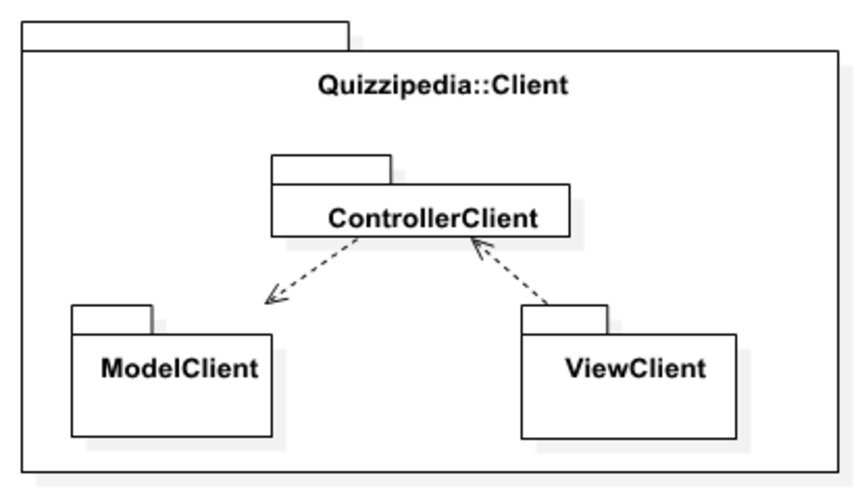
\includegraphics[width=\textwidth]{Img/quizzipedia-client.pdf}}
\caption[Quizzipedia::Client]{Schema Componente Quizzipedia::Client}
\end{figure}
\subsection{Quizzipedia::Client::ModelClient}
Rappresenta il modello dei dati che verranno utilizzati dal sistema lato client.
\begin{figure}[H]
\centering
\noindent\makebox[\textwidth]{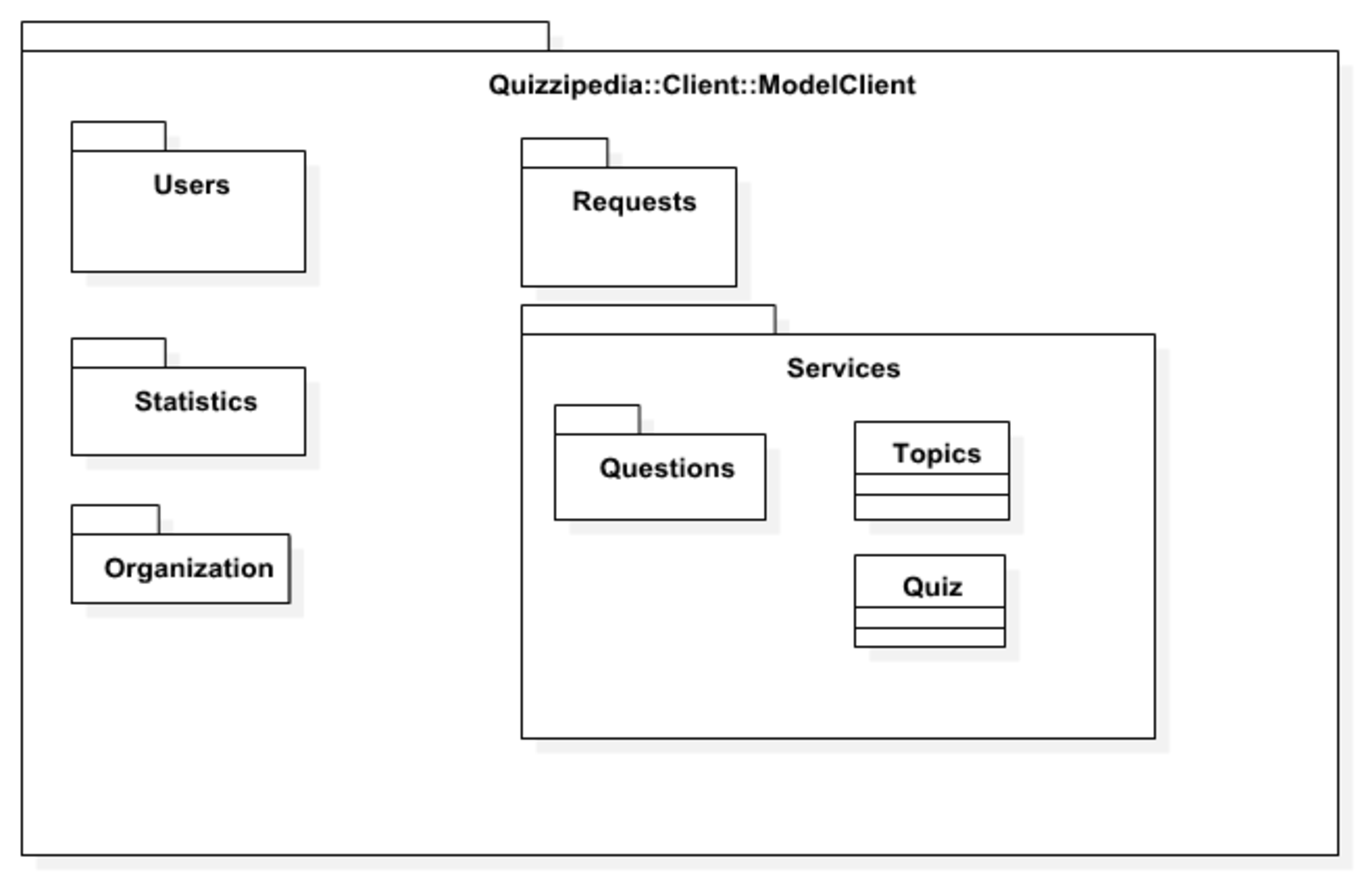
\includegraphics[width=\textwidth]{Img/quizzipedia-client-modelclient.pdf}}
\caption[Quizzipedia::Client::ModelClient]{Schema Componente Quizzipedia::Client::ModelClient}
\end{figure}
\subsubsection{Componenti contenute}
\begin{itemize}
\item Quizzipedia::Client::ModelClient::Organization
\item Quizzipedia::Client::ModelClient::Requests
\item Quizzipedia::Client::ModelClient::Services
\item Quizzipedia::Client::ModelClient::Statistics
\item Quizzipedia::Client::ModelClient::Users
\end{itemize}
\subsection{Quizzipedia::Client::ModelClient::Organization}
La componente gestisce le classi e gli enti, ovvero il sistema in base a cui sono organizzati gli utenti nel sistema.
\begin{figure}[H]
\centering
\noindent\makebox[\textwidth]{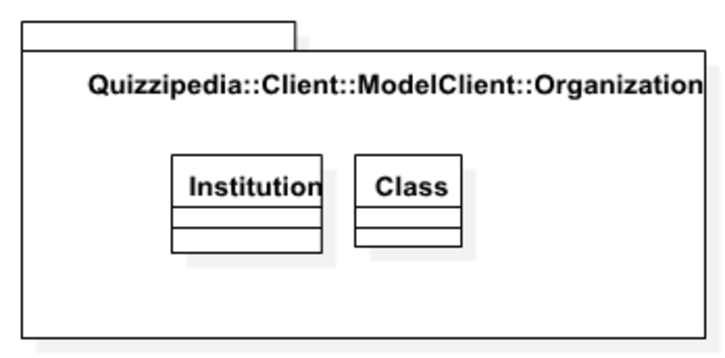
\includegraphics[width=\textwidth]{Img/quizzipedia-client-modelclient-organization.pdf}}
\caption[Quizzipedia::Client::ModelClient::Organization]{Schema Componente Quizzipedia::Client::ModelClient::Organization}
\end{figure}
\subsubsection{Classe Class}
Contiene informazioni relative alla struttura delle classi.
\begin{figure}[H]
\centering
\noindent\makebox[\textwidth]{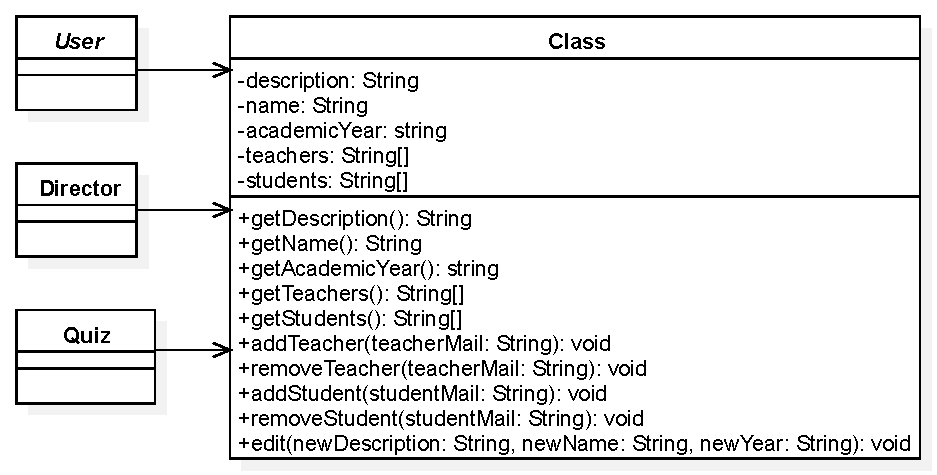
\includegraphics[width=\textwidth]{Img/quizzipedia-client-modelclient-organization-class.pdf}}
\caption{Schema Classe Quizzipedia::Client::ModelClient::Organization::Class}
\end{figure}
\subsubsection{Classe Institution}
La classe contiene le informazioni relative alla struttura dell'ente.
\begin{figure}[H]
\centering
\noindent\makebox[\textwidth]{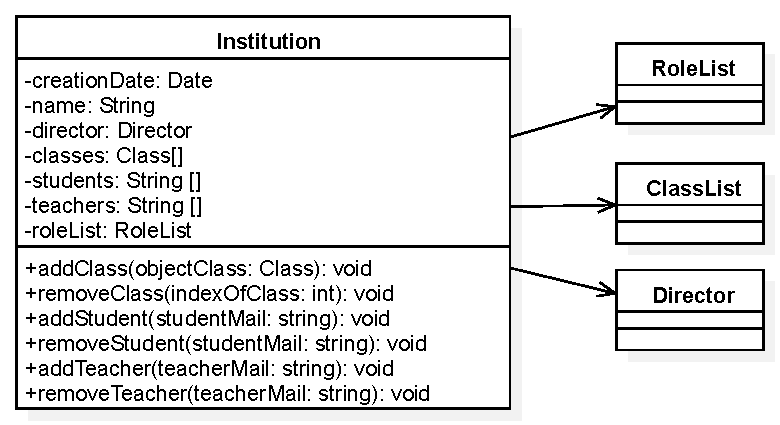
\includegraphics[width=\textwidth]{Img/quizzipedia-client-modelclient-organization-institution.pdf}}
\caption{Schema Classe Quizzipedia::Client::ModelClient::Organization::Institution}
\end{figure}
\subsection{Quizzipedia::Client::ModelClient::Requests}
Questo package contiene le classi necessarie a gestire le richieste di ruolo e di classe degli utenti.
\begin{figure}[H]
\centering
\noindent\makebox[\textwidth]{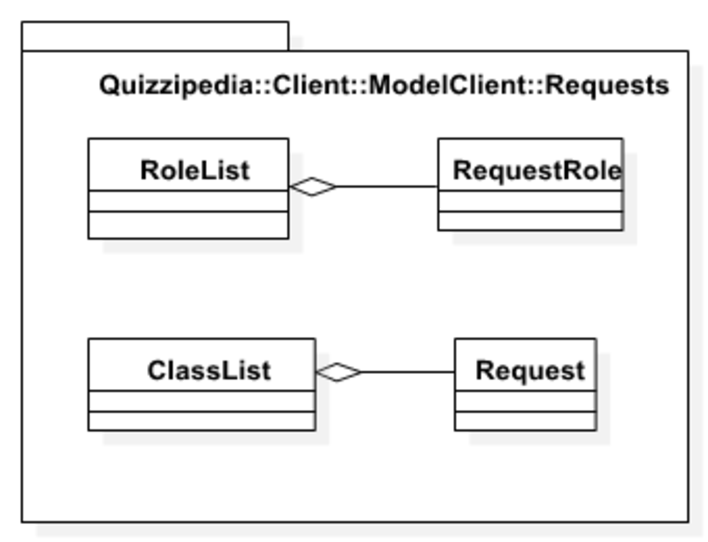
\includegraphics[width=\textwidth]{Img/quizzipedia-client-modelclient-requests.pdf}}
\caption[Quizzipedia::Client::ModelClient::Requests]{Schema Componente Quizzipedia::Client::ModelClient::Requests}
\end{figure}
\subsubsection{Classe ClassList}
Questa classe gestisce le richieste da parte di Docenti o Studenti per l'assegnazione a una specifica classe.
\begin{figure}[H]
\centering
\noindent\makebox[\textwidth]{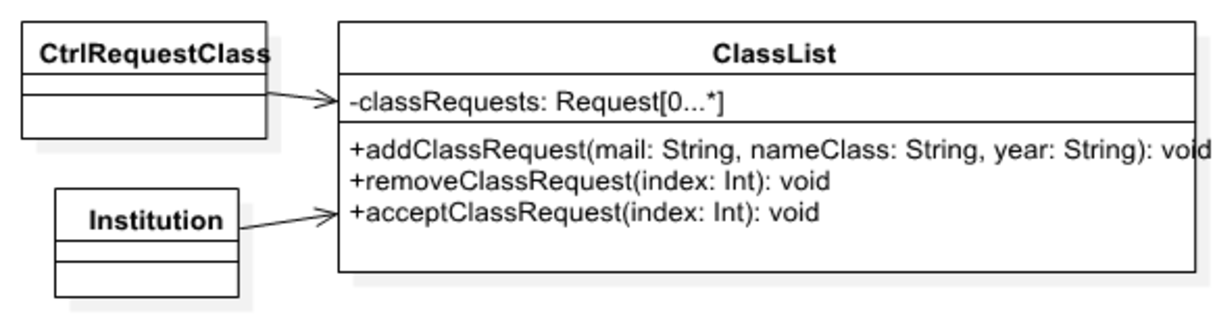
\includegraphics[width=\textwidth]{Img/quizzipedia-client-modelclient-requests-classlist.pdf}}
\caption{Schema Classe Quizzipedia::Client::ModelClient::Requests::ClassList}
\end{figure}
\subsubsection{Classe Request}
La classe memorizza l'utente che invia la richiesta di inserimento in una classe e la classe per cui ha fatto richiesta.
\begin{figure}[H]
\centering
\noindent\makebox[\textwidth]{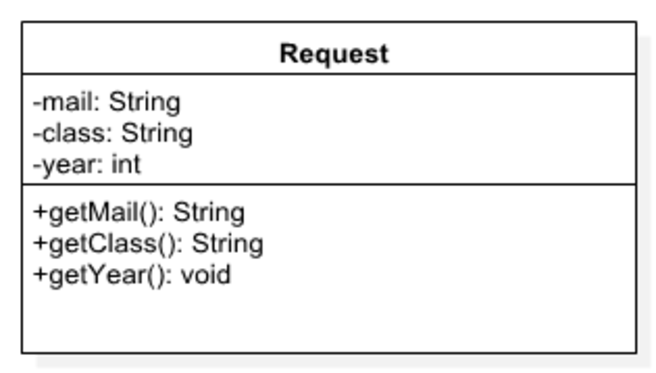
\includegraphics[width=\textwidth]{Img/quizzipedia-client-modelclient-requests-request.pdf}}
\caption{Schema Classe Quizzipedia::Client::ModelClient::Requests::Request}
\end{figure}
\subsubsection{Classe RoleList}
Gli utenti senza ruolo inviano le proprie richieste per l'assegnazione al ruolo di studente o docente al Responsabile di un Ente. Questa classe gestisce tali richieste.
\begin{figure}[H]
\centering
\noindent\makebox[\textwidth]{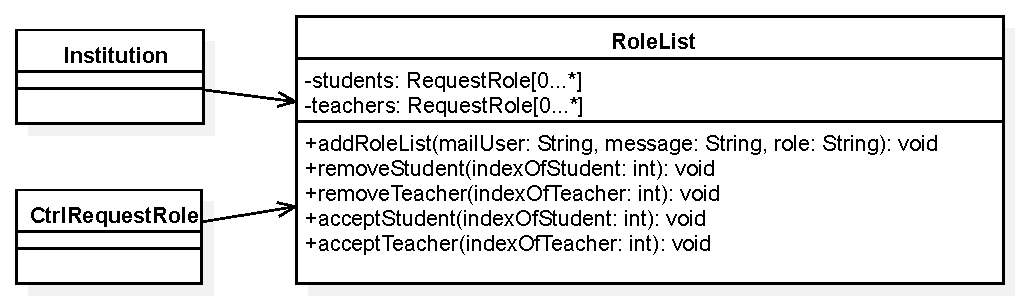
\includegraphics[width=\textwidth]{Img/quizzipedia-client-modelclient-requests-rolelist.pdf}}
\caption{Schema Classe Quizzipedia::Client::ModelClient::Requests::RoleList}
\end{figure}
\subsection{Quizzipedia::Client::ModelClient::Services}
Il package racchiude i modelli necessari alla creazione di domande e quiz, i servizi principali offerti dal nostro prodotto.
\begin{figure}[H]
\centering
\noindent\makebox[\textwidth]{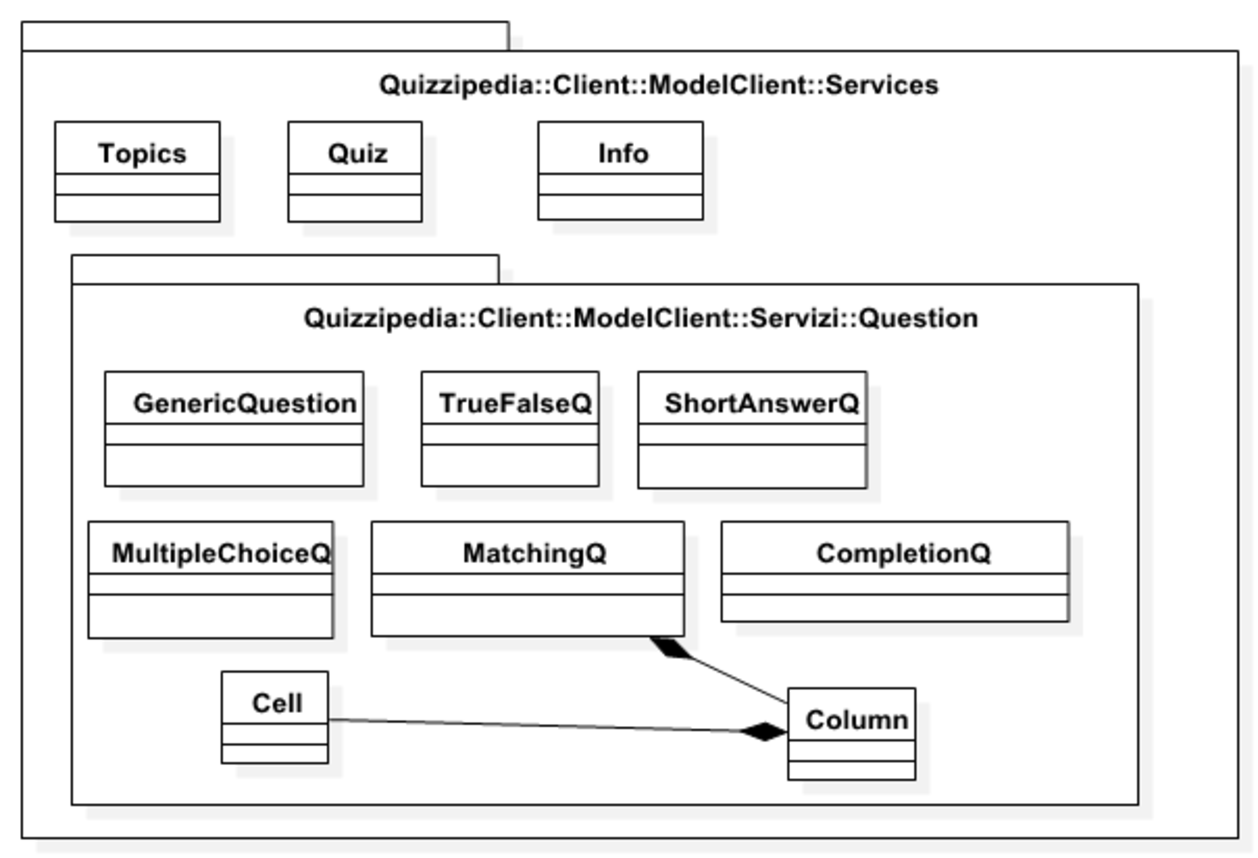
\includegraphics[width=\textwidth]{Img/quizzipedia-client-modelclient-services.pdf}}
\caption[Quizzipedia::Client::ModelClient::Services]{Schema Componente Quizzipedia::Client::ModelClient::Services}
\end{figure}
\subsubsection{Componenti contenute}
\begin{itemize}
\item Quizzipedia::Client::ModelClient::Services::Questions
\end{itemize}
\subsubsection{Classe Info}
Riassume le informazioni principali su quiz e domande, necessarie per una presentazione sintetica e puntuale all'utente. È poi possibile risalire alla domanda o al quiz completi.
\begin{figure}[H]
\centering
\noindent\makebox[\textwidth]{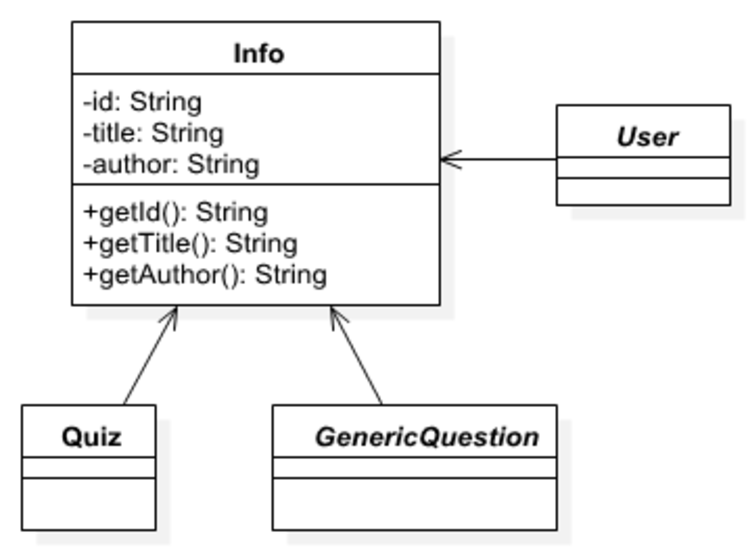
\includegraphics[width=\textwidth]{Img/quizzipedia-client-modelclient-services-info.pdf}}
\caption{Schema Classe Quizzipedia::Client::ModelClient::Services::Info}
\end{figure}
\subsubsection{Classe Quiz}
Include la struttura del quiz.
\begin{figure}[H]
\centering
\noindent\makebox[\textwidth]{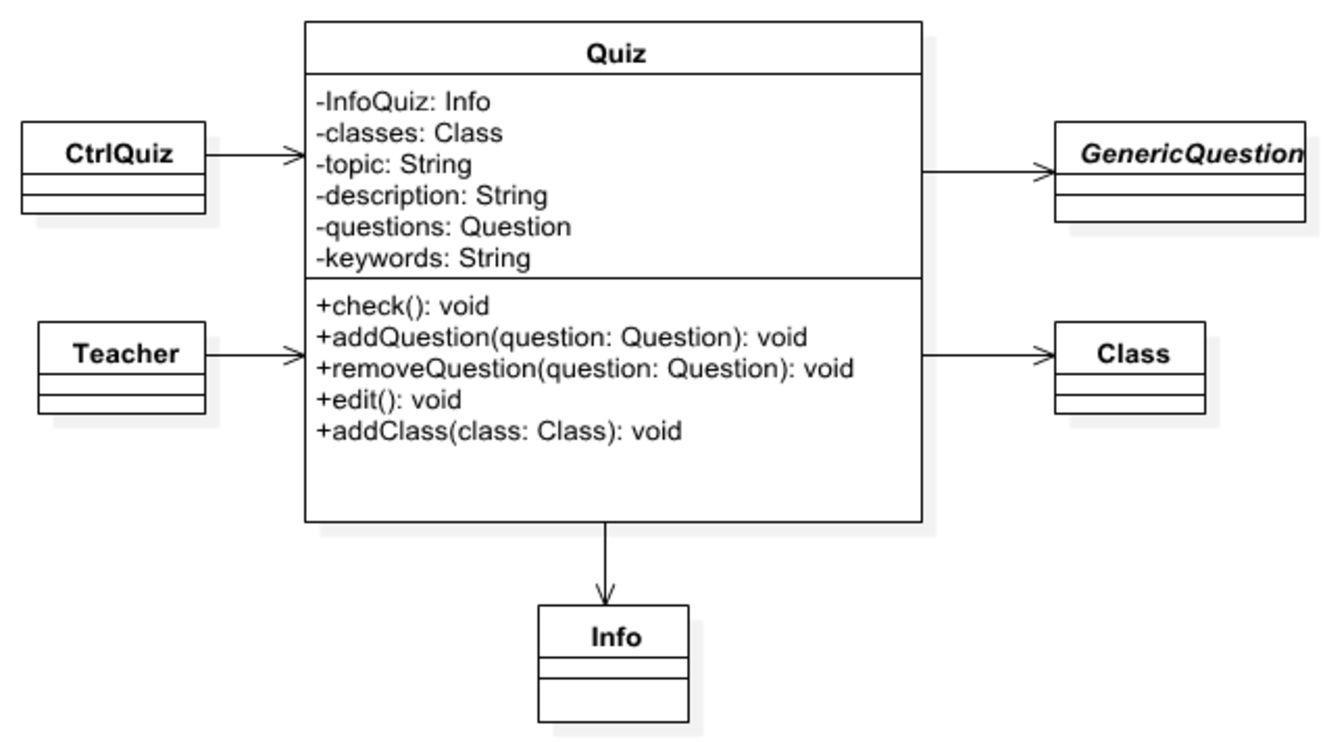
\includegraphics[width=\textwidth]{Img/quizzipedia-client-modelclient-services-quiz.pdf}}
\caption{Schema Classe Quizzipedia::Client::ModelClient::Services::Quiz}
\end{figure}
\subsubsection{Classe Topics}
Modella la struttura necessaria a memorizzare la lista di argomenti. A ogni domanda e a ogni quiz verranno poi associati i relativi argomenti .
\begin{figure}[H]
\centering
\noindent\makebox[\textwidth]{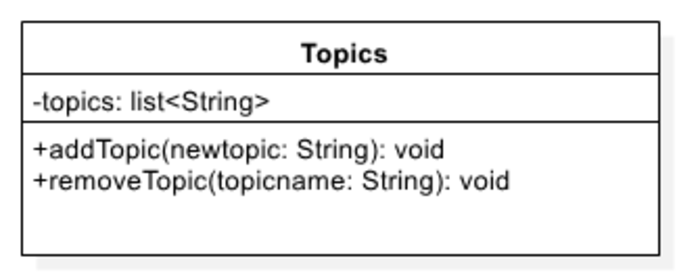
\includegraphics[width=\textwidth]{Img/quizzipedia-client-modelclient-services-topics.pdf}}
\caption{Schema Classe Quizzipedia::Client::ModelClient::Services::Topics}
\end{figure}
\subsection{Quizzipedia::Client::ModelClient::Services::Questions}
Descrive il modo in cui sono strutturati i vari tipi di domande che l'utente può incontrare durante la creazione o la compilazione di quiz.
\begin{figure}[H]
\centering
\noindent\makebox[\textwidth]{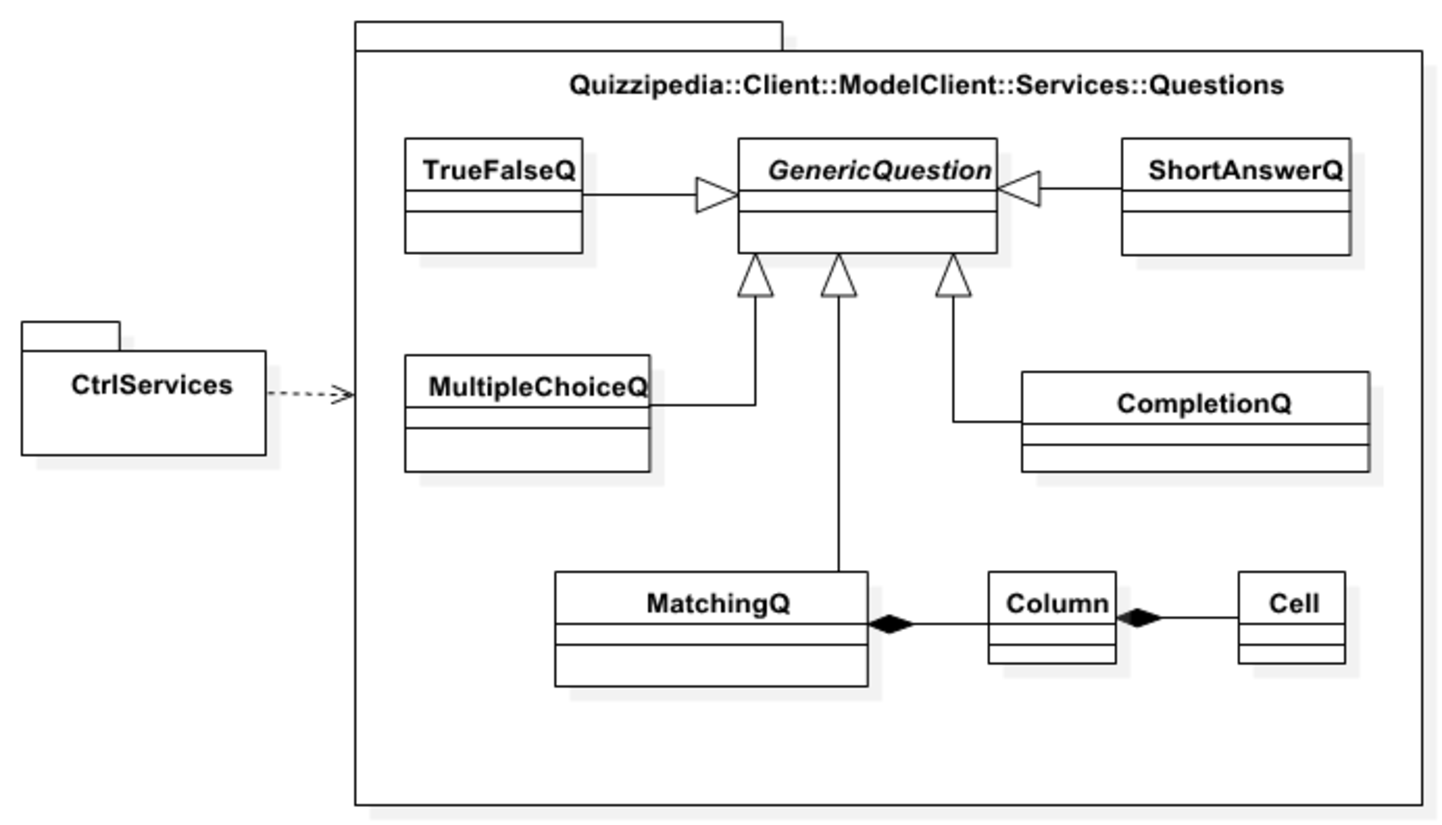
\includegraphics[width=\textwidth]{Img/quizzipedia-client-modelclient-services-questions.pdf}}
\caption[Quizzipedia::Client::ModelClient::Services::Questions]{Schema Componente Quizzipedia::Client::ModelClient::Services::Questions}
\end{figure}
\subsubsection{Classe Cell}
La classe descrive ogni singola riga (quindi ogni opzione) della colonna della domanda a collegamento.
\begin{figure}[H]
\centering
\noindent\makebox[\textwidth]{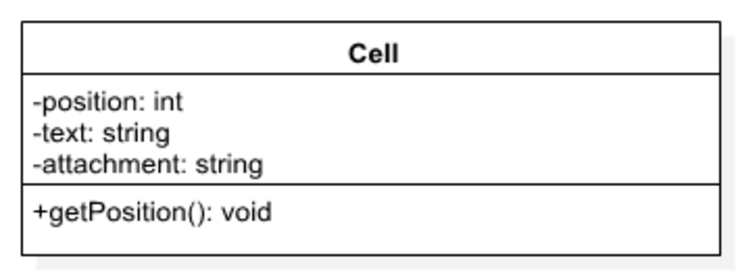
\includegraphics[width=\textwidth]{Img/quizzipedia-client-modelclient-services-questions-cell.pdf}}
\caption{Schema Classe Quizzipedia::Client::ModelClient::Services::Questions::Cell}
\end{figure}
\subsubsection{Classe Column}
La classe descrive le colonne della domanda a collegamenti.
\begin{figure}[H]
\centering
\noindent\makebox[\textwidth]{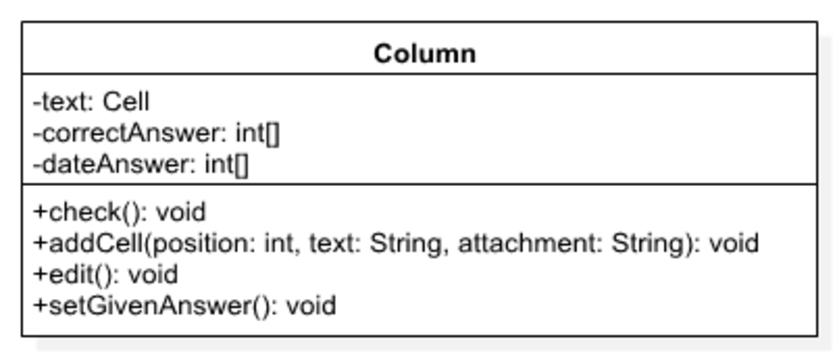
\includegraphics[width=\textwidth]{Img/quizzipedia-client-modelclient-services-questions-column.pdf}}
\caption{Schema Classe Quizzipedia::Client::ModelClient::Services::Questions::Column}
\end{figure}
\subsubsection{Classe CompletionQ}
Descrive le domande a completamento. Il docente fornirà un testo incompleto e una lista di possibili completamenti; lo studente dovrà inserire le parole adeguate nella giusta posizione.
\begin{figure}[H]
\centering
\noindent\makebox[\textwidth]{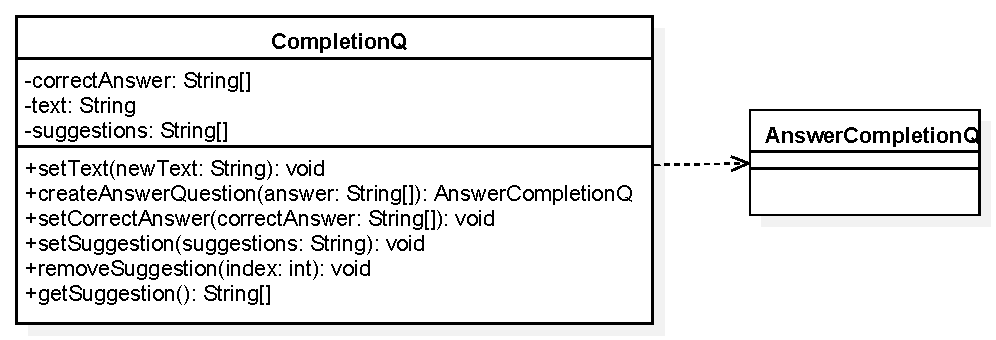
\includegraphics[width=\textwidth]{Img/quizzipedia-client-modelclient-services-questions-completionq.pdf}}
\caption{Schema Classe Quizzipedia::Client::ModelClient::Services::Questions::CompletionQ}
\end{figure}
\subsubsection{Classe GenericQuestion}
Descrive le parti comuni a tutti i tipi di domanda presenti nel sistema.
\begin{figure}[H]
\centering
\noindent\makebox[\textwidth]{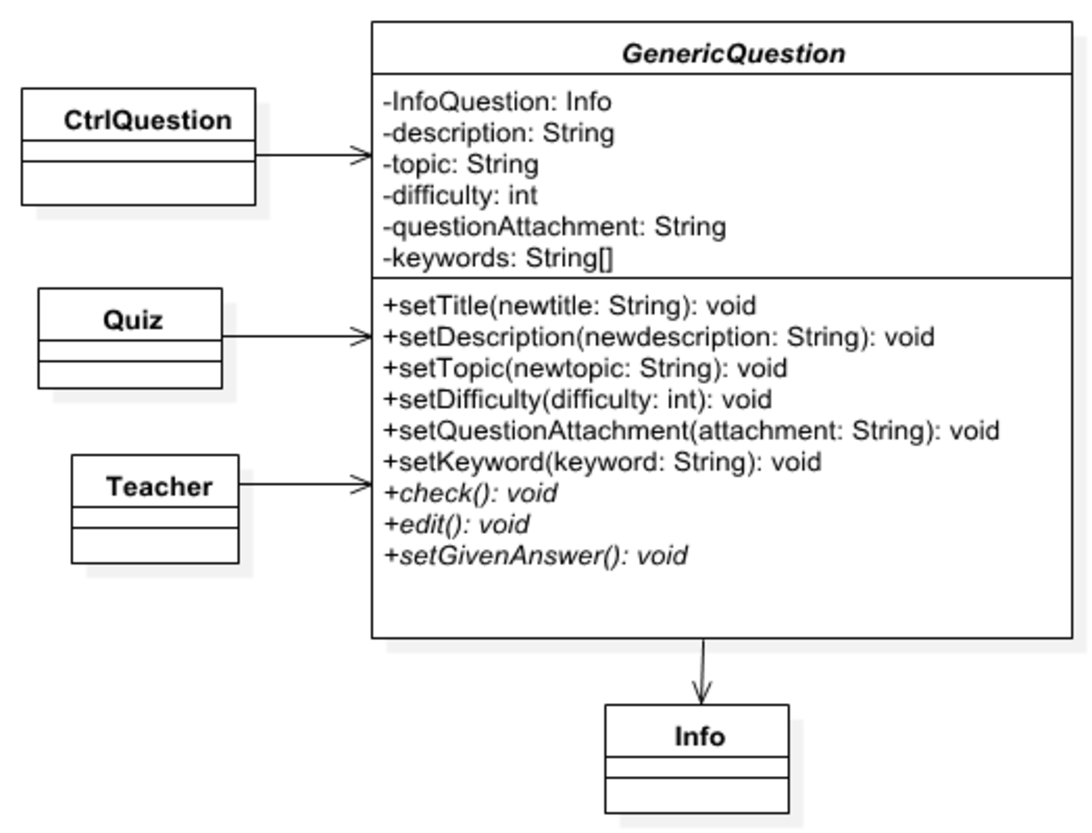
\includegraphics[width=\textwidth]{Img/quizzipedia-client-modelclient-services-questions-genericquestion.pdf}}
\caption{Schema Classe Quizzipedia::Client::ModelClient::Services::Questions::GenericQuestion}
\end{figure}
\subsubsection{Classe MatchingQ}
La struttura descrive le domande a collegamento. L'utente dovrà formare la risposa collegando entrate da un numero variabile di colonne .
\begin{figure}[H]
\centering
\noindent\makebox[\textwidth]{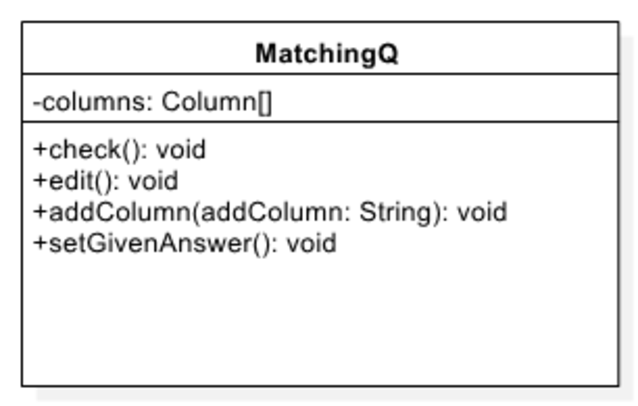
\includegraphics[width=\textwidth]{Img/quizzipedia-client-modelclient-services-questions-matchingq.pdf}}
\caption{Schema Classe Quizzipedia::Client::ModelClient::Services::Questions::MatchingQ}
\end{figure}
\subsubsection{Classe MultipleChoiceQ}
La struttura descrive le domande a scelta multipla; viene presentata una lista di opzioni tra cui scegliere quelle corrette.
\begin{figure}[H]
\centering
\noindent\makebox[\textwidth]{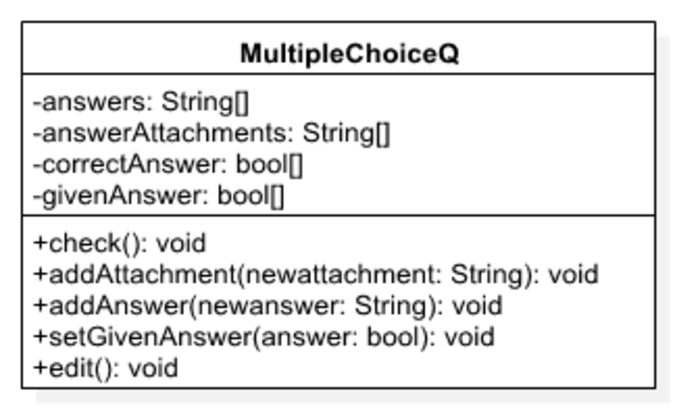
\includegraphics[width=\textwidth]{Img/quizzipedia-client-modelclient-services-questions-multiplechoiceq.pdf}}
\caption{Schema Classe Quizzipedia::Client::ModelClient::Services::Questions::MultipleChoiceQ}
\end{figure}
\subsubsection{Classe ShortAnswerQ}
La struttura descrive le domande aperte, ovvero quelle la cui risposta consiste in un termine o una frase specifici.
\begin{figure}[H]
\centering
\noindent\makebox[\textwidth]{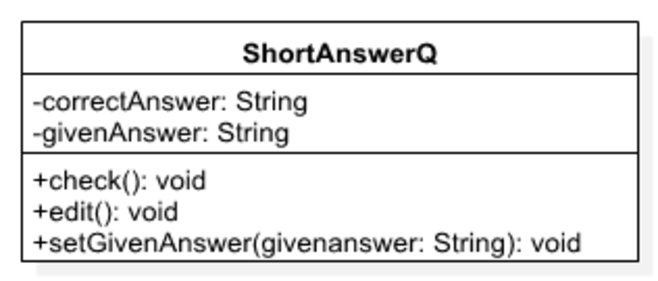
\includegraphics[width=\textwidth]{Img/quizzipedia-client-modelclient-services-questions-shortanswerq.pdf}}
\caption{Schema Classe Quizzipedia::Client::ModelClient::Services::Questions::ShortAnswerQ}
\end{figure}
\subsubsection{Classe TrueFalseQ}
Viene descritta la struttura delle domande che prevedono di decidere la veridicità di un'affermazione.
\begin{figure}[H]
\centering
\noindent\makebox[\textwidth]{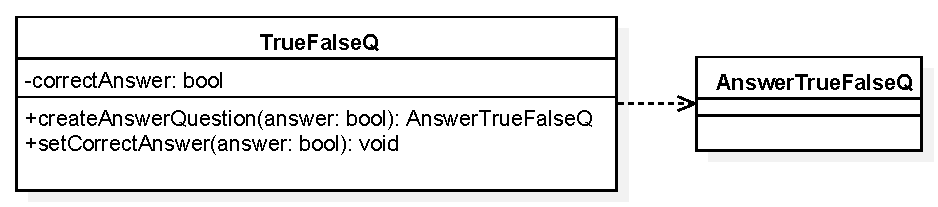
\includegraphics[width=\textwidth]{Img/quizzipedia-client-modelclient-services-questions-truefalseq.pdf}}
\caption{Schema Classe Quizzipedia::Client::ModelClient::Services::Questions::TrueFalseQ}
\end{figure}
\subsection{Quizzipedia::Client::ModelClient::Statistics}
Qui sono raccolte le classi con il compito di reperire informazioni sulle statistiche dal server e presentarle al'utente finale. Sono disponibili statistiche per le domande, per i quiz e per gli studenti di ogni classe.
\begin{figure}[H]
\centering
\noindent\makebox[\textwidth]{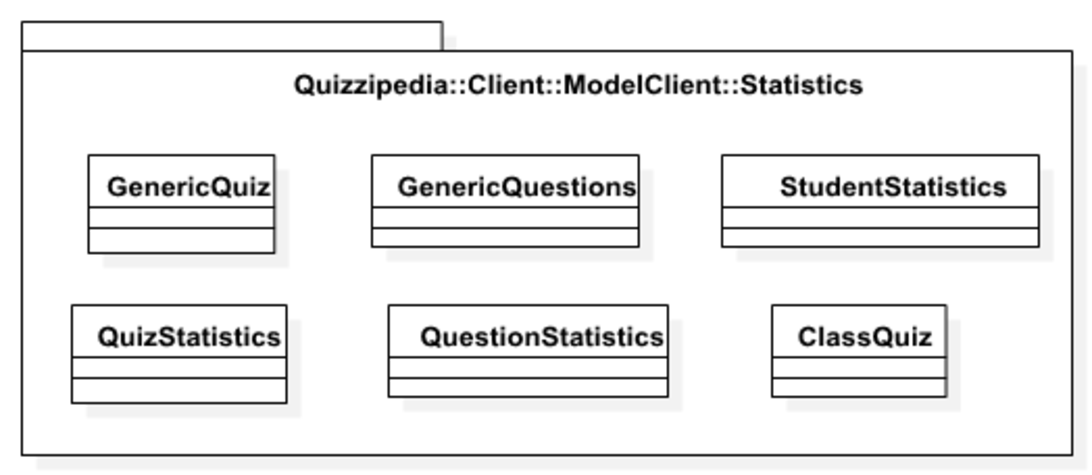
\includegraphics[width=\textwidth]{Img/quizzipedia-client-modelclient-statistics.pdf}}
\caption[Quizzipedia::Client::ModelClient::Statistics]{Schema Componente Quizzipedia::Client::ModelClient::Statistics}
\end{figure}
\subsubsection{Classe ClassQuiz}
La classe raccoglie le statistiche riguardanti gli studenti di una classe relativamente a un quiz assegnato.
\begin{figure}[H]
\centering
\noindent\makebox[\textwidth]{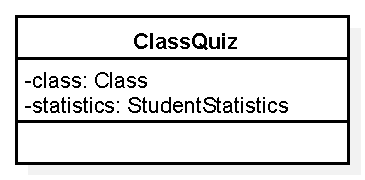
\includegraphics[width=\textwidth]{Img/quizzipedia-client-modelclient-statistics-classquiz.pdf}}
\caption{Schema Classe Quizzipedia::Client::ModelClient::Statistics::ClassQuiz}
\end{figure}
\subsubsection{Classe QuestionGenerics}
Le statistiche relative a più domande vengono raccolte e organizzate per permetterne la visualizzazione agli utenti.
\begin{figure}[H]
\centering
\noindent\makebox[\textwidth]{\includegraphics[width=\textwidth]{Img/quizzipedia-client-modelclient-statistics-questiongenerics.pdf}}
\caption{Schema Classe Quizzipedia::Client::ModelClient::Statistics::QuestionGenerics}
\end{figure}
\subsubsection{Classe QuestionStatistics}
La classe raccoglie le statistiche principali riguardanti una singola domanda. Da qui è poi possibile risalire alla domanda.
\begin{figure}[H]
\centering
\noindent\makebox[\textwidth]{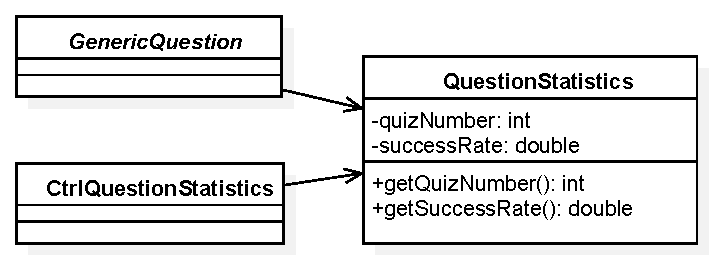
\includegraphics[width=\textwidth]{Img/quizzipedia-client-modelclient-statistics-questionstatistics.pdf}}
\caption{Schema Classe Quizzipedia::Client::ModelClient::Statistics::QuestionStatistics}
\end{figure}
\subsubsection{Classe QuizGenerics}
Le statistiche relative a più quiz vengono raccolte e organizzate per permetterne la visualizzazione agli utenti.
\begin{figure}[H]
\centering
\noindent\makebox[\textwidth]{\includegraphics[width=\textwidth]{Img/quizzipedia-client-modelclient-statistics-quizgenerics.pdf}}
\caption{Schema Classe Quizzipedia::Client::ModelClient::Statistics::QuizGenerics}
\end{figure}
\subsubsection{Classe QuizStatistics}
La classe raccoglie le statistiche principali riguardanti un singolo quiz. Da qui è poi possibile ottenere il quiz in questione.
\begin{figure}[H]
\centering
\noindent\makebox[\textwidth]{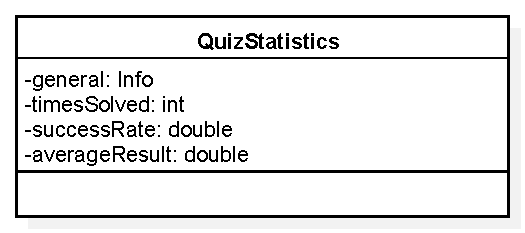
\includegraphics[width=\textwidth]{Img/quizzipedia-client-modelclient-statistics-quizstatistics.pdf}}
\caption{Schema Classe Quizzipedia::Client::ModelClient::Statistics::QuizStatistics}
\end{figure}
\subsubsection{Classe StudentStatistics}
Qui è memorizzata la struttura che permette di associare a un utente le statistiche riguardanti un quiz (voto, superamento).
\begin{figure}[H]
\centering
\noindent\makebox[\textwidth]{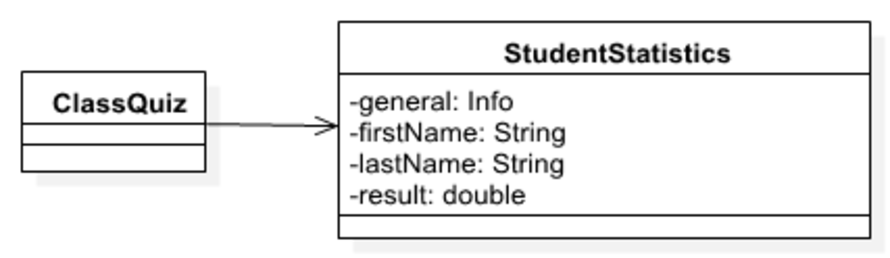
\includegraphics[width=\textwidth]{Img/quizzipedia-client-modelclient-statistics-studentstatistics.pdf}}
\caption{Schema Classe Quizzipedia::Client::ModelClient::Statistics::StudentStatistics}
\end{figure}
\subsection{Quizzipedia::Client::ModelClient::Users}
Raccoglie le classi necessarie a descrivere le diverse tipologie di utente che possono accedere al sistema.
\begin{figure}[H]
\centering
\noindent\makebox[\textwidth]{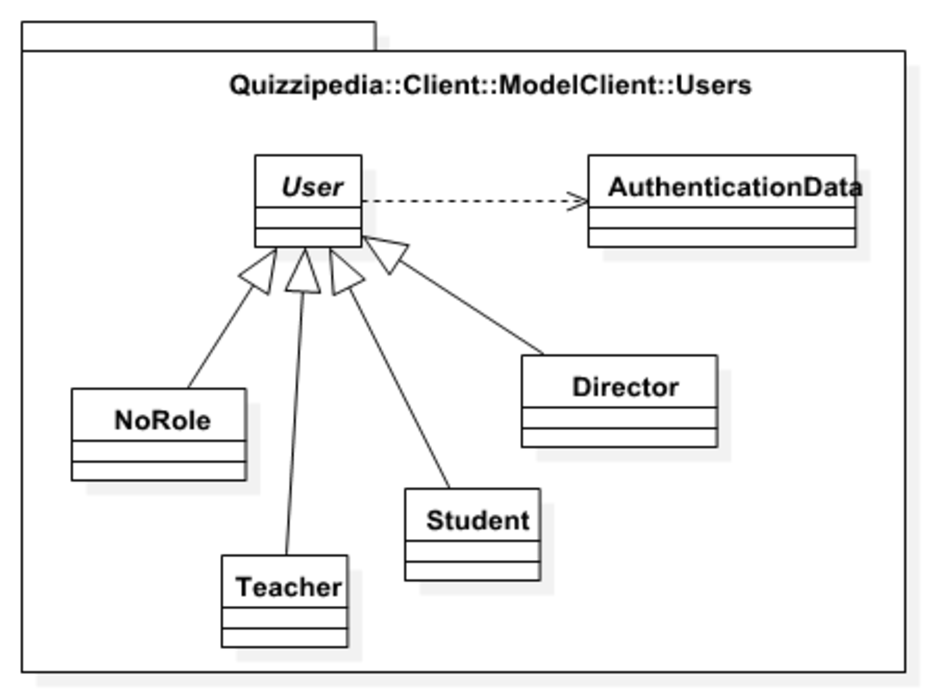
\includegraphics[width=\textwidth]{Img/quizzipedia-client-modelclient-users.pdf}}
\caption[Quizzipedia::Client::ModelClient::Users]{Schema Componente Quizzipedia::Client::ModelClient::Users}
\end{figure}
\subsubsection{Interazioni con altre componenti}
\begin{itemize}
\item Quizzipedia::Client::ModelClient::Organization
\item Quizzipedia::Client::ModelClient::Requests
\item Quizzipedia::Client::ModelClient::Services
\item Quizzipedia::Client::ModelClient::Statistics
\end{itemize}
\subsubsection{Classe AuthenticationData}
Questa classe gestisce le informazioni di autenticazione comuni a tutti gli utenti.
\begin{figure}[H]
\centering
\noindent\makebox[\textwidth]{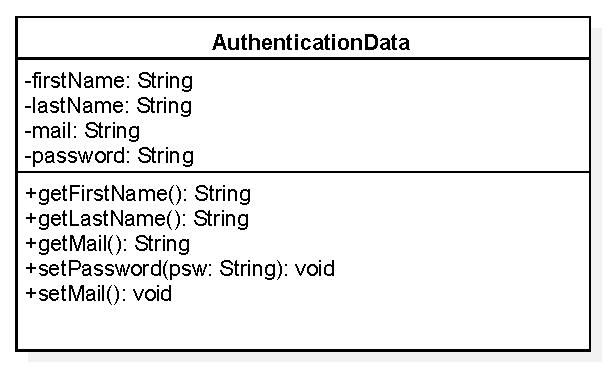
\includegraphics[width=\textwidth]{Img/quizzipedia-client-modelclient-users-authenticationdata.pdf}}
\caption{Schema Classe Quizzipedia::Client::ModelClient::Users::AuthenticationData}
\end{figure}
\subsubsection{Classe Director}
Rappresenta un Responsabile, ovvero colui che gestisce Docenti e Studenti per ogni Ente del sistema.
\begin{figure}[H]
\centering
\noindent\makebox[\textwidth]{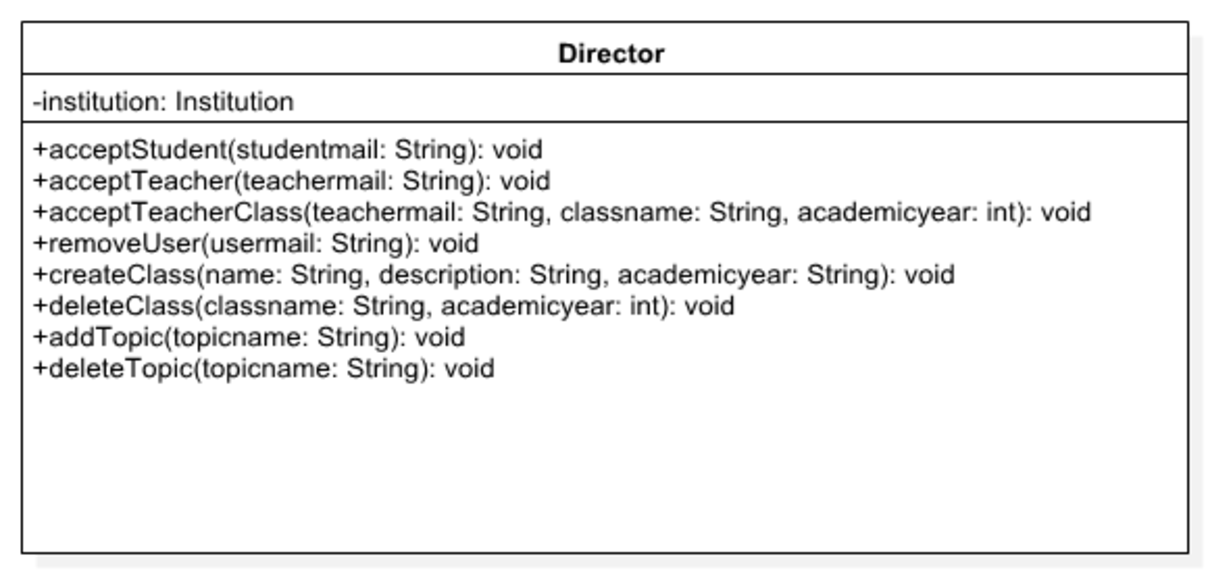
\includegraphics[width=\textwidth]{Img/quizzipedia-client-modelclient-users-director.pdf}}
\caption{Schema Classe Quizzipedia::Client::ModelClient::Users::Director}
\end{figure}
\subsubsection{Classe NoRole}
Rappresenta gli utenti senza ruolo del sistema; ovvero coloro che si sono registrati e autenticati ma non hanno ancora fatto richiesta per l'assegnazione ad alcun ruolo.
\begin{figure}[H]
\centering
\noindent\makebox[\textwidth]{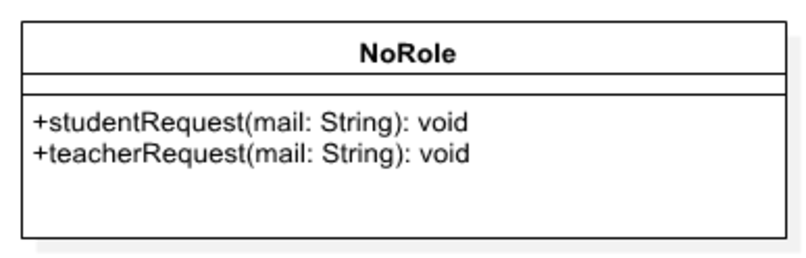
\includegraphics[width=\textwidth]{Img/quizzipedia-client-modelclient-users-norole.pdf}}
\caption{Schema Classe Quizzipedia::Client::ModelClient::Users::NoRole}
\end{figure}
\subsubsection{Classe Student}
Rappresenta uno studente del sistema e implementa le sue funzioni specifiche oltre a quelle ereditate da Utente.
\begin{figure}[H]
\centering
\noindent\makebox[\textwidth]{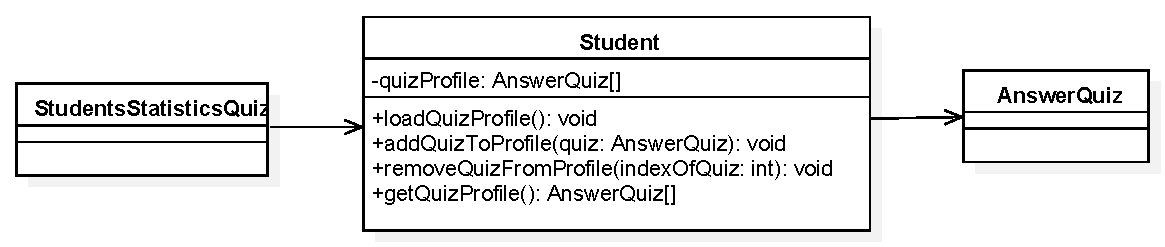
\includegraphics[width=\textwidth]{Img/quizzipedia-client-modelclient-users-student.pdf}}
\caption{Schema Classe Quizzipedia::Client::ModelClient::Users::Student}
\end{figure}
\subsubsection{Classe Teacher}
Rappresenta un docente del sistema e ne implementa le funzionalità specifiche in aggiunta a quelle comuni a tutti gli utenti.
\begin{figure}[H]
\centering
\noindent\makebox[\textwidth]{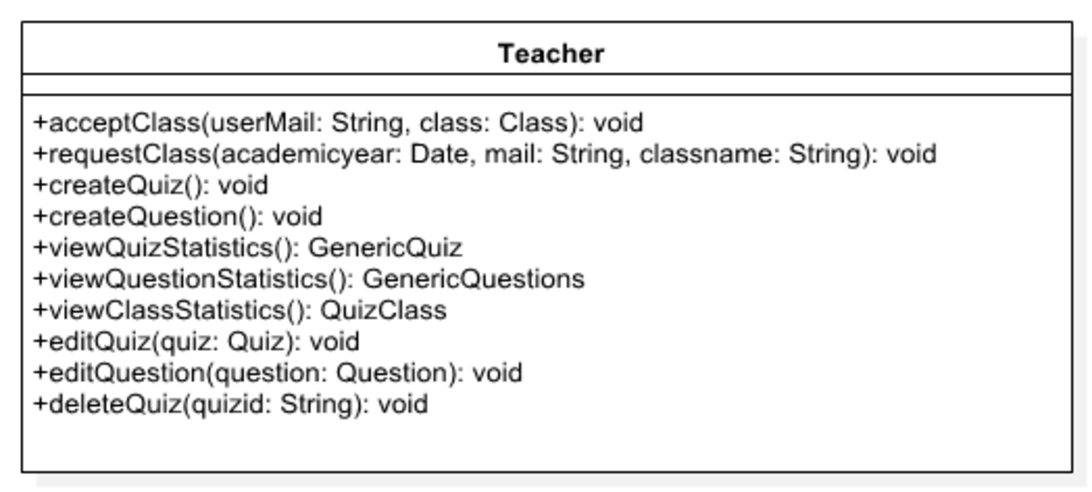
\includegraphics[width=\textwidth]{Img/quizzipedia-client-modelclient-users-teacher.pdf}}
\caption{Schema Classe Quizzipedia::Client::ModelClient::Users::Teacher}
\end{figure}
\subsubsection{Classe User}
Questa è una classe astratta e raccoglie le funzionalità comuni a tutti gli utenti.
\begin{figure}[H]
\centering
\noindent\makebox[\textwidth]{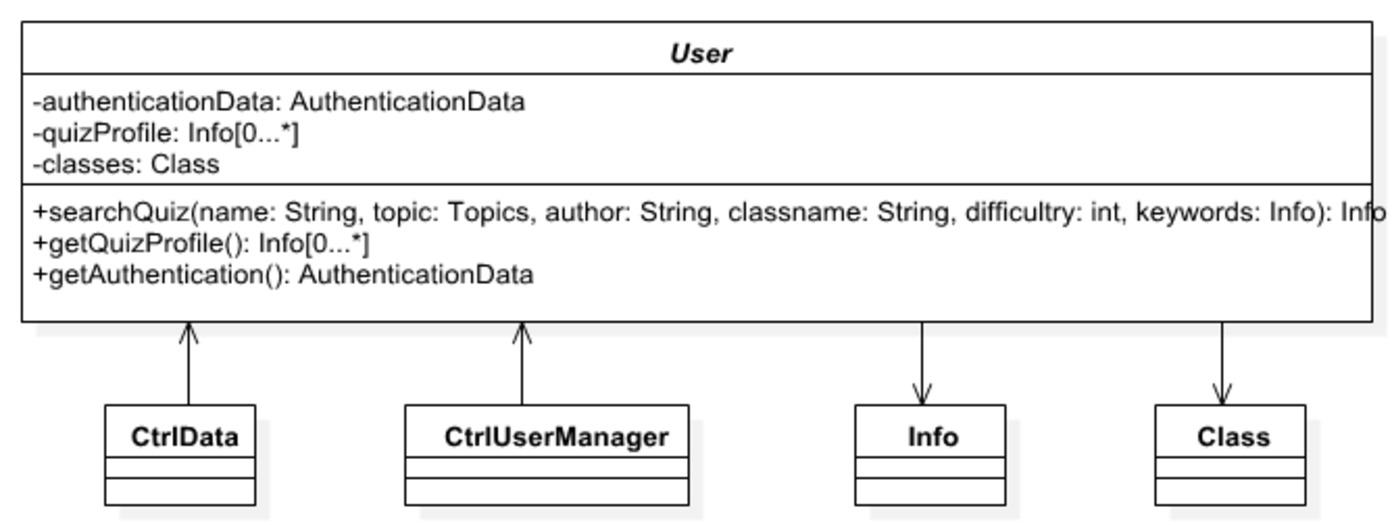
\includegraphics[width=\textwidth]{Img/quizzipedia-client-modelclient-users-user.pdf}}
\caption{Schema Classe Quizzipedia::Client::ModelClient::Users::User}
\end{figure}
\subsection{Quizzipedia::Client::ViewClient}
Racchiude tutte le componenti necessarie per presentare il prodotto all'utente.
\begin{figure}[H]
\centering
\noindent\makebox[\textwidth]{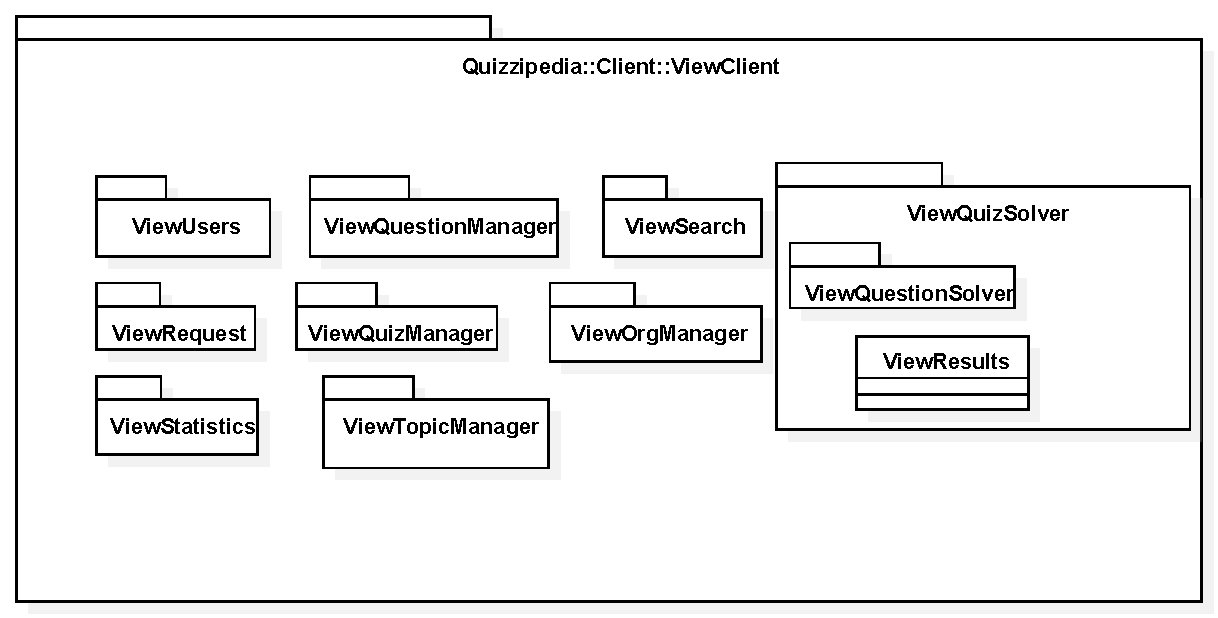
\includegraphics[width=\textwidth]{Img/quizzipedia-client-viewclient.pdf}}
\caption[Quizzipedia::Client::ViewClient]{Schema Componente Quizzipedia::Client::ViewClient}
\end{figure}
\subsubsection{Componenti contenute}
\begin{itemize}
\item Quizzipedia::Client::ViewClient::ViewErrors
\item Quizzipedia::Client::ViewClient::ViewOrgManager
\item Quizzipedia::Client::ViewClient::ViewQuestionManager
\item Quizzipedia::Client::ViewClient::ViewQuizManager
\item Quizzipedia::Client::ViewClient::ViewQuizSolver
\item Quizzipedia::Client::ViewClient::ViewRequests
\item Quizzipedia::Client::ViewClient::ViewSearch
\item Quizzipedia::Client::ViewClient::ViewStatistics
\item Quizzipedia::Client::ViewClient::ViewTopicManager
\item Quizzipedia::Client::ViewClient::ViewUsers
\end{itemize}
\subsubsection{Interazioni con altre componenti}
\begin{itemize}
\item Quizzipedia::Client::ControllerClient
\end{itemize}
\subsection{Quizzipedia::Client::ViewClient::ViewErrors}
Il package raccoglie tutte le finestre di errore che il sistema può, eventualmente, visualizzare.
\begin{figure}[H]
\centering
\noindent\makebox[\textwidth]{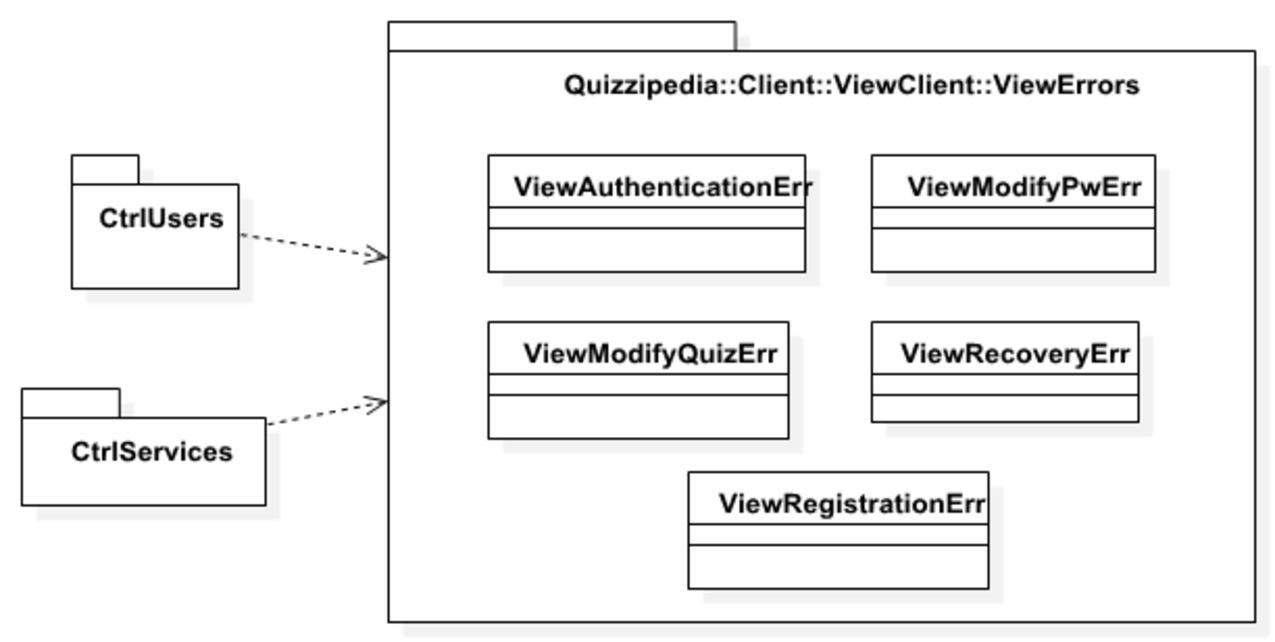
\includegraphics[width=\textwidth]{Img/quizzipedia-client-viewclient-viewerrors.pdf}}
\caption[Quizzipedia::Client::ViewClient::ViewErrors]{Schema Componente Quizzipedia::Client::ViewClient::ViewErrors}
\end{figure}
\subsubsection{Classe ViewAuthenticationErr}
La classe si occupa della visualizzazione del messaggio di errore in fase di autenticazione.
\begin{figure}[H]
\centering
\noindent\makebox[\textwidth]{\includegraphics[width=\textwidth]{Img/quizzipedia-client-viewclient-viewerrors-viewauthenticationerr.pdf}}
\caption{Schema Classe Quizzipedia::Client::ViewClient::ViewErrors::ViewAuthenticationErr}
\end{figure}
\subsubsection{Classe ViewModifyPwErr}
La classe si occupa della visualizzazione del messaggio di errore in fase modifica della password.
\begin{figure}[H]
\centering
\noindent\makebox[\textwidth]{\includegraphics[width=\textwidth]{Img/quizzipedia-client-viewclient-viewerrors-viewmodifypwerr.pdf}}
\caption{Schema Classe Quizzipedia::Client::ViewClient::ViewErrors::ViewModifyPwErr}
\end{figure}
\subsubsection{Classe ViewModifyQuizErr}
La classe si occupa della visualizzazione del messaggio di errore in fase di modifica di un quiz.
\begin{figure}[H]
\centering
\noindent\makebox[\textwidth]{\includegraphics[width=\textwidth]{Img/quizzipedia-client-viewclient-viewerrors-viewmodifyquizerr.pdf}}
\caption{Schema Classe Quizzipedia::Client::ViewClient::ViewErrors::ViewModifyQuizErr}
\end{figure}
\subsubsection{Classe ViewRecoveryErr}
La classe si occupa della visualizzazione del messaggio di errore in fase di recupero password.
\begin{figure}[H]
\centering
\noindent\makebox[\textwidth]{\includegraphics[width=\textwidth]{Img/quizzipedia-client-viewclient-viewerrors-viewrecoveryerr.pdf}}
\caption{Schema Classe Quizzipedia::Client::ViewClient::ViewErrors::ViewRecoveryErr}
\end{figure}
\subsubsection{Classe ViewRegistrationErr}
La classe si occupa della visualizzazione del messaggio di errore in fase di registrazione.
\begin{figure}[H]
\centering
\noindent\makebox[\textwidth]{\includegraphics[width=\textwidth]{Img/quizzipedia-client-viewclient-viewerrors-viewregistrationerr.pdf}}
\caption{Schema Classe Quizzipedia::Client::ViewClient::ViewErrors::ViewRegistrationErr}
\end{figure}
\subsection{Quizzipedia::Client::ViewClient::ViewOrgManager}
Qui sono raccolte le classi responsabili della presentazione delle pagine da cui sarà possibile gestire le classi e gli enti.
\begin{figure}[H]
\centering
\noindent\makebox[\textwidth]{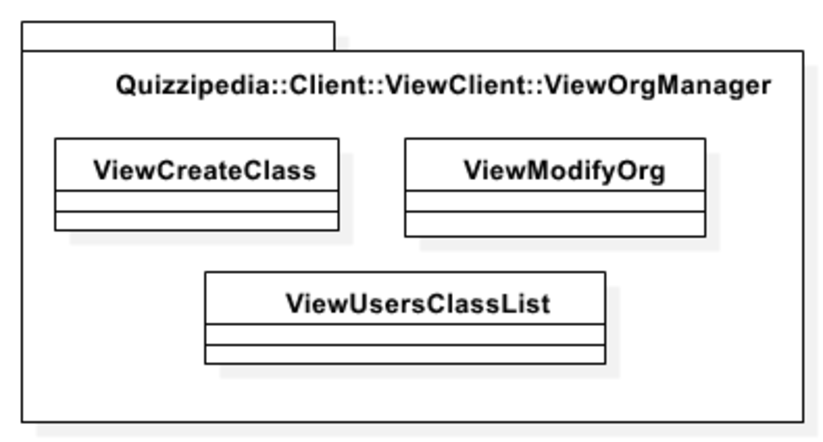
\includegraphics[width=\textwidth]{Img/quizzipedia-client-viewclient-vieworgmanager.pdf}}
\caption[Quizzipedia::Client::ViewClient::ViewOrgManager]{Schema Componente Quizzipedia::Client::ViewClient::ViewOrgManager}
\end{figure}
\subsubsection{Interazioni con altre componenti}
\begin{itemize}
\item Quizzipedia::Client::ControllerClient::CtrlOrganization
\end{itemize}
\subsubsection{Classe ViewCreateClass}
Classe responsabile di creare la pagina da cui sarà possibile creare una nuova classe.
\begin{figure}[H]
\centering
\noindent\makebox[\textwidth]{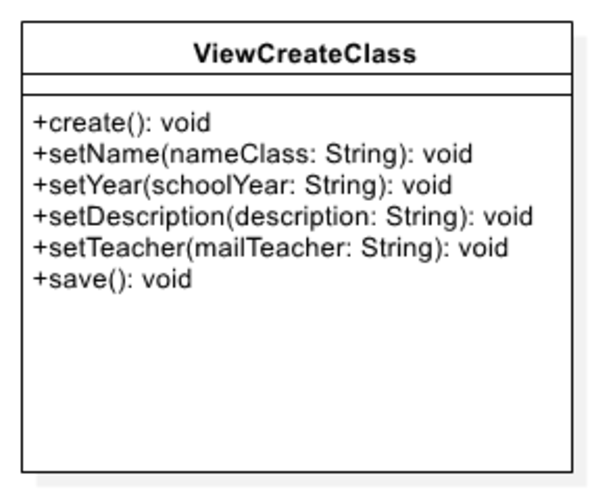
\includegraphics[width=\textwidth]{Img/quizzipedia-client-viewclient-vieworgmanager-viewcreateclass.pdf}}
\caption{Schema Classe Quizzipedia::Client::ViewClient::ViewOrgManager::ViewCreateClass}
\end{figure}
\subsubsection{Classe ViewModifyOrg}
Presenta all'utente la pagina da cui sarà possibile modificare le informazioni su una classe o su un ente esistente.
\begin{figure}[H]
\centering
\noindent\makebox[\textwidth]{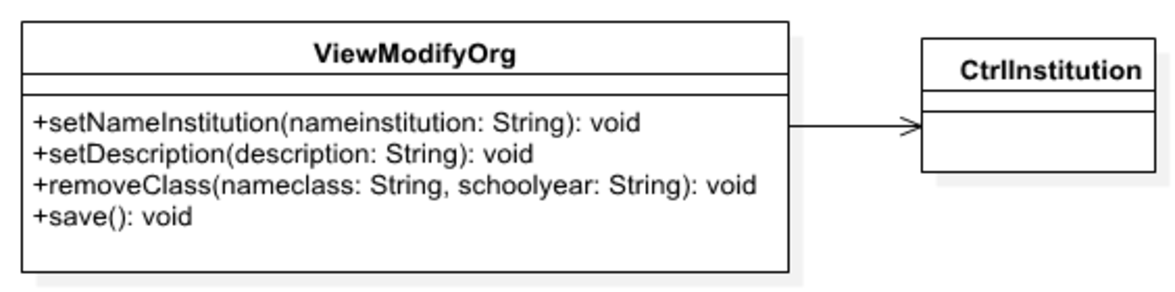
\includegraphics[width=\textwidth]{Img/quizzipedia-client-viewclient-vieworgmanager-viewmodifyorg.pdf}}
\caption{Schema Classe Quizzipedia::Client::ViewClient::ViewOrgManager::ViewModifyOrg}
\end{figure}
\subsubsection{Classe ViewUsersClassList}
La classe si occupa di presentare una lista degli utenti iscritti alla classe e altre informazioni aggiuntive.
\begin{figure}[H]
\centering
\noindent\makebox[\textwidth]{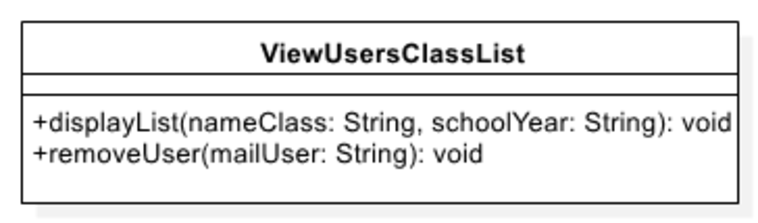
\includegraphics[width=\textwidth]{Img/quizzipedia-client-viewclient-vieworgmanager-viewusersclasslist.pdf}}
\caption{Schema Classe Quizzipedia::Client::ViewClient::ViewOrgManager::ViewUsersClassList}
\end{figure}
\subsection{Quizzipedia::Client::ViewClient::ViewQuestionManager}
Qui sono raccolte le classi responsabili della presentazione delle pagine da cui sarà possibile gestire le domande.
\begin{figure}[H]
\centering
\noindent\makebox[\textwidth]{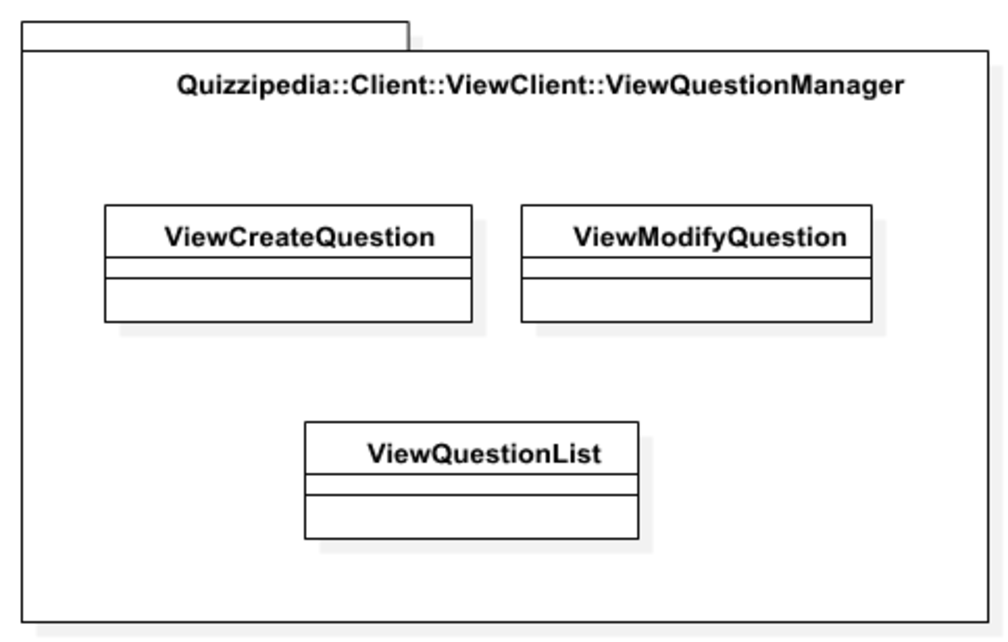
\includegraphics[width=\textwidth]{Img/quizzipedia-client-viewclient-viewquestionmanager.pdf}}
\caption[Quizzipedia::Client::ViewClient::ViewQuestionManager]{Schema Componente Quizzipedia::Client::ViewClient::ViewQuestionManager}
\end{figure}
\subsubsection{Interazioni con altre componenti}
\begin{itemize}
\item Quizzipedia::Client::ControllerClient::CtrlServices
\end{itemize}
\subsubsection{Classe ViewCreateQuestion}
Presenta la pagina da cui sarà possibile creare una nuova domanda.
\begin{figure}[H]
\centering
\noindent\makebox[\textwidth]{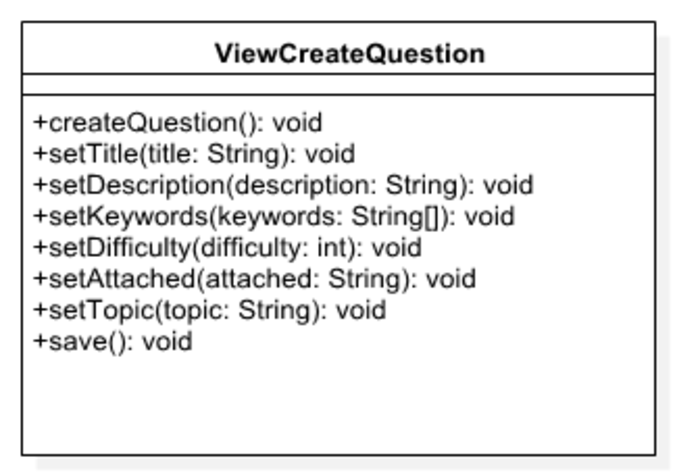
\includegraphics[width=\textwidth]{Img/quizzipedia-client-viewclient-viewquestionmanager-viewcreatequestion.pdf}}
\caption{Schema Classe Quizzipedia::Client::ViewClient::ViewQuestionManager::ViewCreateQuestion}
\end{figure}
\subsubsection{Classe ViewModifyQuestion}
Gestisce la visualizzazione della pagina da cui è possibile modificare una domanda esistente.
\begin{figure}[H]
\centering
\noindent\makebox[\textwidth]{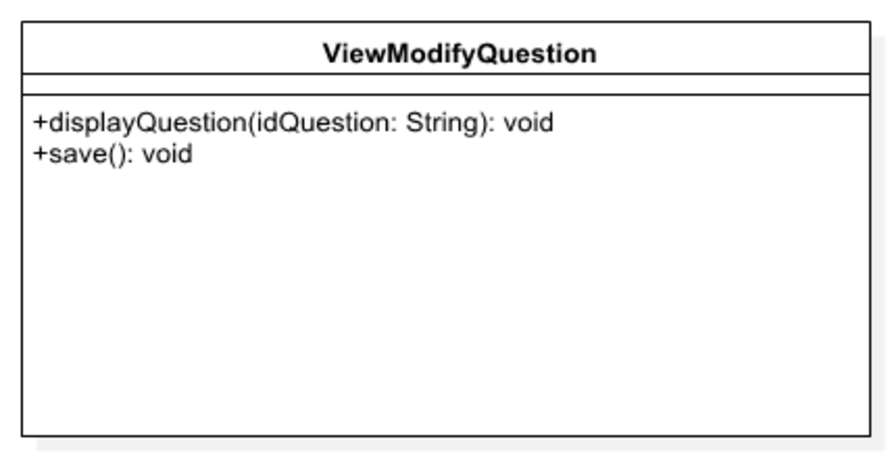
\includegraphics[width=\textwidth]{Img/quizzipedia-client-viewclient-viewquestionmanager-viewmodifyquestion.pdf}}
\caption{Schema Classe Quizzipedia::Client::ViewClient::ViewQuestionManager::ViewModifyQuestion}
\end{figure}
\subsubsection{Classe ViewQuestionList}
Presenta all'utente il pannello da cui sarà possibile visualizzare una lista di informazioni riassuntive sulle domande e compiere alcune operazioni su di esse.
\begin{figure}[H]
\centering
\noindent\makebox[\textwidth]{\includegraphics[width=\textwidth]{Img/quizzipedia-client-viewclient-viewquestionmanager-viewquestionlist.pdf}}
\caption{Schema Classe Quizzipedia::Client::ViewClient::ViewQuestionManager::ViewQuestionList}
\end{figure}
\subsection{Quizzipedia::Client::ViewClient::ViewQuizManager}
Qui sono raccolte le classi responsabili della presentazione delle pagine da cui sarà possibile gestire i quiz.
\begin{figure}[H]
\centering
\noindent\makebox[\textwidth]{\includegraphics[width=\textwidth]{Img/quizzipedia-client-viewclient-viewquizmanager.pdf}}
\caption[Quizzipedia::Client::ViewClient::ViewQuizManager]{Schema Componente Quizzipedia::Client::ViewClient::ViewQuizManager}
\end{figure}
\subsubsection{Interazioni con altre componenti}
\begin{itemize}
\item Quizzipedia::Client::ControllerClient::CtrlServices
\end{itemize}
\subsubsection{Classe ViewCreateQuiz}
Presenta la pagina da cui sarà possibile creare un nuovo quiz.
\begin{figure}[H]
\centering
\noindent\makebox[\textwidth]{\includegraphics[width=\textwidth]{Img/quizzipedia-client-viewclient-viewquizmanager-viewcreatequiz.pdf}}
\caption{Schema Classe Quizzipedia::Client::ViewClient::ViewQuizManager::ViewCreateQuiz}
\end{figure}
\subsubsection{Classe ViewModifyQuiz}
Presenta all'utente una pagina da cui è possibile modificare un quiz esistente.
\begin{figure}[H]
\centering
\noindent\makebox[\textwidth]{\includegraphics[width=\textwidth]{Img/quizzipedia-client-viewclient-viewquizmanager-viewmodifyquiz.pdf}}
\caption{Schema Classe Quizzipedia::Client::ViewClient::ViewQuizManager::ViewModifyQuiz}
\end{figure}
\subsubsection{Classe ViewQuizList}
Carica una pagina contenente una lista con informazioni riassuntive sui quiz e un pannello da cui sarà possibile svolgere delle operazioni sugli stessi.
\begin{figure}[H]
\centering
\noindent\makebox[\textwidth]{\includegraphics[width=\textwidth]{Img/quizzipedia-client-viewclient-viewquizmanager-viewquizlist.pdf}}
\caption{Schema Classe Quizzipedia::Client::ViewClient::ViewQuizManager::ViewQuizList}
\end{figure}
\subsection{Quizzipedia::Client::ViewClient::ViewQuizSolver}
Il package raccoglie le classi necessarie alla visualizzazione delle pagine da cui sarà possibile svolgere quiz.
\begin{figure}[H]
\centering
\noindent\makebox[\textwidth]{\includegraphics[width=\textwidth]{Img/quizzipedia-client-viewclient-viewquizsolver.pdf}}
\caption[Quizzipedia::Client::ViewClient::ViewQuizSolver]{Schema Componente Quizzipedia::Client::ViewClient::ViewQuizSolver}
\end{figure}
\subsubsection{Componenti contenute}
\begin{itemize}
\item Quizzipedia::Client::ViewClient::ViewQuizSolver::ViewQuestionSolver
\end{itemize}
\subsubsection{Interazioni con altre componenti}
\begin{itemize}
\item Quizzipedia::Client::ControllerClient::CtrlServices
\end{itemize}
\subsubsection{Classe ViewResults}
La classe ha il compito di costruire la pagina da cui sarà possibile vedere l'esito di un quiz.
\begin{figure}[H]
\centering
\noindent\makebox[\textwidth]{\includegraphics[width=\textwidth]{Img/quizzipedia-client-viewclient-viewquizsolver-viewresults.pdf}}
\caption{Schema Classe Quizzipedia::Client::ViewClient::ViewQuizSolver::ViewResults}
\end{figure}
\subsection{Quizzipedia::Client::ViewClient::ViewQuizSolver::ViewQuestionSolver}
Il package raccoglie le classi necessarie alla visualizzazione delle pagine da cui sarà possibile rispondere alle singole domande.
\begin{figure}[H]
\centering
\noindent\makebox[\textwidth]{\includegraphics[width=\textwidth]{Img/quizzipedia-client-viewclient-viewquizsolver-viewquestionsolver.pdf}}
\caption[Quizzipedia::Client::ViewClient::ViewQuizSolver::ViewQuestionSolver]{Schema Componente Quizzipedia::Client::ViewClient::ViewQuizSolver::ViewQuestionSolver}
\end{figure}
\subsubsection{Classe ViewCompletionQ}
Presenta all'utente la pagina da cui sarà possibile rispondere a una domanda a completamento.
\begin{figure}[H]
\centering
\noindent\makebox[\textwidth]{\includegraphics[width=\textwidth]{Img/quizzipedia-client-viewclient-viewquizsolver-viewquestionsolver-viewcompletionq.pdf}}
\caption{Schema Classe Quizzipedia::Client::ViewClient::ViewQuizSolver::ViewQuestionSolver::ViewCompletionQ}
\end{figure}
\subsubsection{Classe ViewMatchingQ}
Presenta all'utente la pagina da cui sarà possibile rispondere a una domanda a collegamenti.
\begin{figure}[H]
\centering
\noindent\makebox[\textwidth]{\includegraphics[width=\textwidth]{Img/quizzipedia-client-viewclient-viewquizsolver-viewquestionsolver-viewmatchingq.pdf}}
\caption{Schema Classe Quizzipedia::Client::ViewClient::ViewQuizSolver::ViewQuestionSolver::ViewMatchingQ}
\end{figure}
\subsubsection{Classe ViewMultipleChoiceQ}
Presenta all'utente la pagina da cui sarà possibile rispondere a una domanda a risposta multipla.
\begin{figure}[H]
\centering
\noindent\makebox[\textwidth]{\includegraphics[width=\textwidth]{Img/quizzipedia-client-viewclient-viewquizsolver-viewquestionsolver-viewmultiplechoiceq.pdf}}
\caption{Schema Classe Quizzipedia::Client::ViewClient::ViewQuizSolver::ViewQuestionSolver::ViewMultipleChoiceQ}
\end{figure}
\subsubsection{Classe ViewShortAnswerQ}
Presenta all'utente la pagina da cui sarà possibile rispondere a una domanda a risposta aperta.
\begin{figure}[H]
\centering
\noindent\makebox[\textwidth]{\includegraphics[width=\textwidth]{Img/quizzipedia-client-viewclient-viewquizsolver-viewquestionsolver-viewshortanswerq.pdf}}
\caption{Schema Classe Quizzipedia::Client::ViewClient::ViewQuizSolver::ViewQuestionSolver::ViewShortAnswerQ}
\end{figure}
\subsubsection{Classe ViewTrueFalseQ}
Presenta all'utente la pagina da cui sarà possibile rispondere a una domanda di tipo vero/falso.
\begin{figure}[H]
\centering
\noindent\makebox[\textwidth]{\includegraphics[width=\textwidth]{Img/quizzipedia-client-viewclient-viewquizsolver-viewquestionsolver-viewtruefalseq.pdf}}
\caption{Schema Classe Quizzipedia::Client::ViewClient::ViewQuizSolver::ViewQuestionSolver::ViewTrueFalseQ}
\end{figure}
\subsection{Quizzipedia::Client::ViewClient::ViewRequests}
Qui sono raccolte le pagine che permettono all'utente di gestire le richieste di ruolo e classe.
\begin{figure}[H]
\centering
\noindent\makebox[\textwidth]{\includegraphics[width=\textwidth]{Img/quizzipedia-client-viewclient-viewrequests.pdf}}
\caption[Quizzipedia::Client::ViewClient::ViewRequests]{Schema Componente Quizzipedia::Client::ViewClient::ViewRequests}
\end{figure}
\subsubsection{Interazioni con altre componenti}
\begin{itemize}
\item Quizzipedia::Client::ControllerClient::CtrlRequests
\end{itemize}
\subsubsection{Classe RequestClass}
Costruisce la pagina da cui l'utente potrà richiedere di entrare in una classe.
\begin{figure}[H]
\centering
\noindent\makebox[\textwidth]{\includegraphics[width=\textwidth]{Img/quizzipedia-client-viewclient-viewrequests-requestclass.pdf}}
\caption{Schema Classe Quizzipedia::Client::ViewClient::ViewRequests::RequestClass}
\end{figure}
\subsubsection{Classe RequestRole}
Costruisce la pagina da cui l'utente potrà richiedere un ruolo (studente o docente).
\begin{figure}[H]
\centering
\noindent\makebox[\textwidth]{\includegraphics[width=\textwidth]{Img/quizzipedia-client-viewclient-viewrequests-requestrole.pdf}}
\caption{Schema Classe Quizzipedia::Client::ViewClient::ViewRequests::RequestRole}
\end{figure}
\subsubsection{Classe ViewClassList}
Classe responsabile della visualizzazione del pannello da cui sarà possibile gestire le richieste di inserimento in una classe.
\begin{figure}[H]
\centering
\noindent\makebox[\textwidth]{\includegraphics[width=\textwidth]{Img/quizzipedia-client-viewclient-viewrequests-viewclasslist.pdf}}
\caption{Schema Classe Quizzipedia::Client::ViewClient::ViewRequests::ViewClassList}
\end{figure}
\subsubsection{Classe ViewRolesList}
Classe responsabile della visualizzazione del pannello da cui sarà possibile gestire le richieste di assegnazione di ruolo.
\begin{figure}[H]
\centering
\noindent\makebox[\textwidth]{\includegraphics[width=\textwidth]{Img/quizzipedia-client-viewclient-viewrequests-viewroleslist.pdf}}
\caption{Schema Classe Quizzipedia::Client::ViewClient::ViewRequests::ViewRolesList}
\end{figure}
\subsection{Quizzipedia::Client::ViewClient::ViewSearch}
Il package contiene le classi responsabili della creazione delle pagine da cui sarà possibile ricercare domande, quiz e classi .
\begin{figure}[H]
\centering
\noindent\makebox[\textwidth]{\includegraphics[width=\textwidth]{Img/quizzipedia-client-viewclient-viewsearch.pdf}}
\caption[Quizzipedia::Client::ViewClient::ViewSearch]{Schema Componente Quizzipedia::Client::ViewClient::ViewSearch}
\end{figure}
\subsubsection{Interazioni con altre componenti}
\begin{itemize}
\item Quizzipedia::Client::ControllerClient::CtrlOrganization
\item Quizzipedia::Client::ControllerClient::CtrlServices
\end{itemize}
\subsubsection{Classe ViewSearchClass}
La classe carica la pagina da cui sarà possibile ricercare classi all'interno di un ente.
\begin{figure}[H]
\centering
\noindent\makebox[\textwidth]{\includegraphics[width=\textwidth]{Img/quizzipedia-client-viewclient-viewsearch-viewsearchclass.pdf}}
\caption{Schema Classe Quizzipedia::Client::ViewClient::ViewSearch::ViewSearchClass}
\end{figure}
\subsubsection{Classe ViewSearchQuestion}
Classe che ha il compito di caricare la pagina da cui sarà possibile effettuare la ricerca di domande.
\begin{figure}[H]
\centering
\noindent\makebox[\textwidth]{\includegraphics[width=\textwidth]{Img/quizzipedia-client-viewclient-viewsearch-viewsearchquestion.pdf}}
\caption{Schema Classe Quizzipedia::Client::ViewClient::ViewSearch::ViewSearchQuestion}
\end{figure}
\subsubsection{Classe ViewSearchQuiz}
Raccoglie i metodi necessari alla creazione della pagina da cui sarà possibile cercare un quiz.
\begin{figure}[H]
\centering
\noindent\makebox[\textwidth]{\includegraphics[width=\textwidth]{Img/quizzipedia-client-viewclient-viewsearch-viewsearchquiz.pdf}}
\caption{Schema Classe Quizzipedia::Client::ViewClient::ViewSearch::ViewSearchQuiz}
\end{figure}
\subsection{Quizzipedia::Client::ViewClient::ViewStatistics}
Package che gestisce le pagine in cui verranno visualizzate le statistiche.
\begin{figure}[H]
\centering
\noindent\makebox[\textwidth]{\includegraphics[width=\textwidth]{Img/quizzipedia-client-viewclient-viewstatistics.pdf}}
\caption[Quizzipedia::Client::ViewClient::ViewStatistics]{Schema Componente Quizzipedia::Client::ViewClient::ViewStatistics}
\end{figure}
\subsubsection{Interazioni con altre componenti}
\begin{itemize}
\item Quizzipedia::Client::ControllerClient::CtrlStatistics
\end{itemize}
\subsubsection{Classe ViewClassStats}
Vengono rappresentate le statistiche relative a una singola classe in relazione a un particolare quiz.
\begin{figure}[H]
\centering
\noindent\makebox[\textwidth]{\includegraphics[width=\textwidth]{Img/quizzipedia-client-viewclient-viewstatistics-viewclassstats.pdf}}
\caption{Schema Classe Quizzipedia::Client::ViewClient::ViewStatistics::ViewClassStats}
\end{figure}
\subsubsection{Classe ViewQuestionStats}
Vengono rappresentate le statistiche generali relative alle domande.
\begin{figure}[H]
\centering
\noindent\makebox[\textwidth]{\includegraphics[width=\textwidth]{Img/quizzipedia-client-viewclient-viewstatistics-viewquestionstats.pdf}}
\caption{Schema Classe Quizzipedia::Client::ViewClient::ViewStatistics::ViewQuestionStats}
\end{figure}
\subsubsection{Classe ViewQuizStats}
Vengono rappresentate le statistiche generali riguardanti i quiz.
\begin{figure}[H]
\centering
\noindent\makebox[\textwidth]{\includegraphics[width=\textwidth]{Img/quizzipedia-client-viewclient-viewstatistics-viewquizstats.pdf}}
\caption{Schema Classe Quizzipedia::Client::ViewClient::ViewStatistics::ViewQuizStats}
\end{figure}
\subsection{Quizzipedia::Client::ViewClient::ViewTopicManager}
Qui sono raccolte le classi responsabili della presentazione delle pagine da cui sarà possibile gestire gli argomenti di domande e quiz.
\begin{figure}[H]
\centering
\noindent\makebox[\textwidth]{\includegraphics[width=\textwidth]{Img/quizzipedia-client-viewclient-viewtopicmanager.pdf}}
\caption[Quizzipedia::Client::ViewClient::ViewTopicManager]{Schema Componente Quizzipedia::Client::ViewClient::ViewTopicManager}
\end{figure}
\subsubsection{Interazioni con altre componenti}
\begin{itemize}
\item Quizzipedia::Client::ControllerClient::CtrlServices
\end{itemize}
\subsubsection{Classe ViewCreateTopic}
La classe caricherà la pagina da cui sarà possibile creare un nuovo argomento.
\begin{figure}[H]
\centering
\noindent\makebox[\textwidth]{\includegraphics[width=\textwidth]{Img/quizzipedia-client-viewclient-viewtopicmanager-viewcreatetopic.pdf}}
\caption{Schema Classe Quizzipedia::Client::ViewClient::ViewTopicManager::ViewCreateTopic}
\end{figure}
\subsubsection{Classe ViewTopicList}
La classe è responsabile della creazione della pagina da cui sarà possibile vedere la lista degli argomenti disponibili.
\begin{figure}[H]
\centering
\noindent\makebox[\textwidth]{\includegraphics[width=\textwidth]{Img/quizzipedia-client-viewclient-viewtopicmanager-viewtopiclist.pdf}}
\caption{Schema Classe Quizzipedia::Client::ViewClient::ViewTopicManager::ViewTopicList}
\end{figure}
\subsection{Quizzipedia::Client::ViewClient::ViewUsers}
Raccoglie le classi necessarie a presentare all'utente le pagine da cui visualizzare le informazioni che lo riguardano e compiere le funzioni principali.
\begin{figure}[H]
\centering
\noindent\makebox[\textwidth]{\includegraphics[width=\textwidth]{Img/quizzipedia-client-viewclient-viewusers.pdf}}
\caption[Quizzipedia::Client::ViewClient::ViewUsers]{Schema Componente Quizzipedia::Client::ViewClient::ViewUsers}
\end{figure}
\subsubsection{Interazioni con altre componenti}
\begin{itemize}
\item Quizzipedia::Client::ControllerClient::CtrlUsers
\end{itemize}
\subsubsection{Classe Login}
Presenta la pagina necessaria per effettuare il login nel sistema.
\begin{figure}[H]
\centering
\noindent\makebox[\textwidth]{\includegraphics[width=\textwidth]{Img/quizzipedia-client-viewclient-viewusers-login.pdf}}
\caption{Schema Classe Quizzipedia::Client::ViewClient::ViewUsers::Login}
\end{figure}
\subsubsection{Classe Logout}
Presenta la pagina necessaria per effettuare il logout dal sistema.
\begin{figure}[H]
\centering
\noindent\makebox[\textwidth]{\includegraphics[width=\textwidth]{Img/quizzipedia-client-viewclient-viewusers-logout.pdf}}
\caption{Schema Classe Quizzipedia::Client::ViewClient::ViewUsers::Logout}
\end{figure}
\subsubsection{Classe Menu}
Presenta all'utente il menu da cui potrà svolgere le proprie funzioni principali.
\begin{figure}[H]
\centering
\noindent\makebox[\textwidth]{\includegraphics[width=\textwidth]{Img/quizzipedia-client-viewclient-viewusers-menu.pdf}}
\caption{Schema Classe Quizzipedia::Client::ViewClient::ViewUsers::Menu}
\end{figure}
\subsubsection{Classe PersonalData}
La classe presenta all'utente la pagina da cui prendere visione delle proprie informazioni personali.
\begin{figure}[H]
\centering
\noindent\makebox[\textwidth]{\includegraphics[width=\textwidth]{Img/quizzipedia-client-viewclient-viewusers-personaldata.pdf}}
\caption{Schema Classe Quizzipedia::Client::ViewClient::ViewUsers::PersonalData}
\end{figure}
\subsubsection{Classe RecoveryPw}
Da questa pagina sarà possibile inserire i dati per il recupero della password.
\begin{figure}[H]
\centering
\noindent\makebox[\textwidth]{\includegraphics[width=\textwidth]{Img/quizzipedia-client-viewclient-viewusers-recoverypw.pdf}}
\caption{Schema Classe Quizzipedia::Client::ViewClient::ViewUsers::RecoveryPw}
\end{figure}
\subsubsection{Classe Registration}
Presenta la pagina da cui effettuare la  registrazione al sistema.
\begin{figure}[H]
\centering
\noindent\makebox[\textwidth]{\includegraphics[width=\textwidth]{Img/quizzipedia-client-viewclient-viewusers-registration.pdf}}
\caption{Schema Classe Quizzipedia::Client::ViewClient::ViewUsers::Registration}
\end{figure}
\subsubsection{Classe ViewModifyUser}
Da qui, grazie ai metodi della classe, l'utente potrà modificare le proprie informazioni personali.
\begin{figure}[H]
\centering
\noindent\makebox[\textwidth]{\includegraphics[width=\textwidth]{Img/quizzipedia-client-viewclient-viewusers-viewmodifyuser.pdf}}
\caption{Schema Classe Quizzipedia::Client::ViewClient::ViewUsers::ViewModifyUser}
\end{figure}
\subsubsection{Classe ViewUsersList}
Presenta un pannello da cui è possibile visualizzare una lista di utenti e compiere operazioni su di loro.
\begin{figure}[H]
\centering
\noindent\makebox[\textwidth]{\includegraphics[width=\textwidth]{Img/quizzipedia-client-viewclient-viewusers-viewuserslist.pdf}}
\caption{Schema Classe Quizzipedia::Client::ViewClient::ViewUsers::ViewUsersList}
\end{figure}
\subsection{Quizzipedia::Client::ControllerClient}
Raccoglie le classi responsabili della comunicazione tra il model e la view.
\begin{figure}[H]
\centering
\noindent\makebox[\textwidth]{\includegraphics[width=\textwidth]{Img/quizzipedia-client-controllerclient.pdf}}
\caption[Quizzipedia::Client::ControllerClient]{Schema Componente Quizzipedia::Client::ControllerClient}
\end{figure}
\subsubsection{Componenti contenute}
\begin{itemize}
\item Quizzipedia::Client::ControllerClient::CtrlOrganization
\item Quizzipedia::Client::ControllerClient::CtrlRequests
\item Quizzipedia::Client::ControllerClient::CtrlServices
\item Quizzipedia::Client::ControllerClient::CtrlStatistics
\item Quizzipedia::Client::ControllerClient::CtrlUsers
\end{itemize}
\subsubsection{Interazioni con altre componenti}
\begin{itemize}
\item Quizzipedia::Client::ModelClient
\end{itemize}
\subsection{Quizzipedia::Client::ControllerClient::CtrlOrganization}
Raccoglie le classi che si occupano delle comunicazioni necessarie per la creazione di enti e classi.
\begin{figure}[H]
\centering
\noindent\makebox[\textwidth]{\includegraphics[width=\textwidth]{Img/quizzipedia-client-controllerclient-ctrlorganization.pdf}}
\caption[Quizzipedia::Client::ControllerClient::CtrlOrganization]{Schema Componente Quizzipedia::Client::ControllerClient::CtrlOrganization}
\end{figure}
\subsubsection{Classe CtrlClass}
Vi sono presenti metodi necessari alla creazione delle classi.
\begin{figure}[H]
\centering
\noindent\makebox[\textwidth]{\includegraphics[width=\textwidth]{Img/quizzipedia-client-controllerclient-ctrlorganization-ctrlclass.pdf}}
\caption{Schema Classe Quizzipedia::Client::ControllerClient::CtrlOrganization::CtrlClass}
\end{figure}
\subsubsection{Classe CtrlInstitution}
Vi sono presenti metodi necessari alla creazione degli enti.
\begin{figure}[H]
\centering
\noindent\makebox[\textwidth]{\includegraphics[width=\textwidth]{Img/quizzipedia-client-controllerclient-ctrlorganization-ctrlinstitution.pdf}}
\caption{Schema Classe Quizzipedia::Client::ControllerClient::CtrlOrganization::CtrlInstitution}
\end{figure}
\subsection{Quizzipedia::Client::ControllerClient::CtrlRequests}
Questo package contiene classi necessarie alla gestione delle richieste di ruolo o classe.
\begin{figure}[H]
\centering
\noindent\makebox[\textwidth]{\includegraphics[width=\textwidth]{Img/quizzipedia-client-controllerclient-ctrlrequests.pdf}}
\caption[Quizzipedia::Client::ControllerClient::CtrlRequests]{Schema Componente Quizzipedia::Client::ControllerClient::CtrlRequests}
\end{figure}
\subsubsection{Classe CtrlRequestClass}
Si occupa delle comunicazioni necessarie per la gestione delle richieste di inserimento in una classe.
\begin{figure}[H]
\centering
\noindent\makebox[\textwidth]{\includegraphics[width=\textwidth]{Img/quizzipedia-client-controllerclient-ctrlrequests-ctrlrequestclass.pdf}}
\caption{Schema Classe Quizzipedia::Client::ControllerClient::CtrlRequests::CtrlRequestClass}
\end{figure}
\subsubsection{Classe CtrlRequestRole}
Si occupa delle comunicazioni necessarie per la gestione delle richieste di ruolo.
\begin{figure}[H]
\centering
\noindent\makebox[\textwidth]{\includegraphics[width=\textwidth]{Img/quizzipedia-client-controllerclient-ctrlrequests-ctrlrequestrole.pdf}}
\caption{Schema Classe Quizzipedia::Client::ControllerClient::CtrlRequests::CtrlRequestRole}
\end{figure}
\subsection{Quizzipedia::Client::ControllerClient::CtrlServices}
Raccoglie gli elementi necessari alla creazione, svolgimento e ricerca di quiz e domande.
\begin{figure}[H]
\centering
\noindent\makebox[\textwidth]{\includegraphics[width=\textwidth]{Img/quizzipedia-client-controllerclient-ctrlservices.pdf}}
\caption[Quizzipedia::Client::ControllerClient::CtrlServices]{Schema Componente Quizzipedia::Client::ControllerClient::CtrlServices}
\end{figure}
\subsubsection{Classe CtrlQuestion}
Fornisce i metodi necessari per la comunicazione tra view e model durante la creazione, modifica e svolgimento di una domanda.
\begin{figure}[H]
\centering
\noindent\makebox[\textwidth]{\includegraphics[width=\textwidth]{Img/quizzipedia-client-controllerclient-ctrlservices-ctrlquestion.pdf}}
\caption{Schema Classe Quizzipedia::Client::ControllerClient::CtrlServices::CtrlQuestion}
\end{figure}
\subsubsection{Classe CtrlQuiz}
Raccoglie i metodi necessari nelle comunicazioni tra view e model richieste per la gestione e lo svolgimento dei quiz.
\begin{figure}[H]
\centering
\noindent\makebox[\textwidth]{\includegraphics[width=\textwidth]{Img/quizzipedia-client-controllerclient-ctrlservices-ctrlquiz.pdf}}
\caption{Schema Classe Quizzipedia::Client::ControllerClient::CtrlServices::CtrlQuiz}
\end{figure}
\subsubsection{Classe CtrlSearch}
La classe contiene i metodi necessari alla comunicazione tra model e view nell'effetuare la ricerca di quiz o domande.
\begin{figure}[H]
\centering
\noindent\makebox[\textwidth]{\includegraphics[width=\textwidth]{Img/quizzipedia-client-controllerclient-ctrlservices-ctrlsearch.pdf}}
\caption{Schema Classe Quizzipedia::Client::ControllerClient::CtrlServices::CtrlSearch}
\end{figure}
\subsubsection{Classe CtrlTopics}
Fornisce i metodi necessari alle comunicazioni richieste per la gestione degli argomenti.
\begin{figure}[H]
\centering
\noindent\makebox[\textwidth]{\includegraphics[width=\textwidth]{Img/quizzipedia-client-controllerclient-ctrlservices-ctrltopics.pdf}}
\caption{Schema Classe Quizzipedia::Client::ControllerClient::CtrlServices::CtrlTopics}
\end{figure}
\subsection{Quizzipedia::Client::ControllerClient::CtrlStatistics}
Raccoglie le classi necessarie a recuperare le statistiche da presentare all'utente.
\begin{figure}[H]
\centering
\noindent\makebox[\textwidth]{\includegraphics[width=\textwidth]{Img/quizzipedia-client-controllerclient-ctrlstatistics.pdf}}
\caption[Quizzipedia::Client::ControllerClient::CtrlStatistics]{Schema Componente Quizzipedia::Client::ControllerClient::CtrlStatistics}
\end{figure}
\subsubsection{Classe CtrlStats}
Classe necessaria al caricamento delle statistiche relative ai quiz, alle domande e alle classi.
\begin{figure}[H]
\centering
\noindent\makebox[\textwidth]{\includegraphics[width=\textwidth]{Img/quizzipedia-client-controllerclient-ctrlstatistics-ctrlstats.pdf}}
\caption{Schema Classe Quizzipedia::Client::ControllerClient::CtrlStatistics::CtrlStats}
\end{figure}
\subsection{Quizzipedia::Client::ControllerClient::CtrlUsers}
Il package raccoglie le classi che permettono la comunicazione per quanto riguarda funzioni e dati dell'utente.
\begin{figure}[H]
\centering
\noindent\makebox[\textwidth]{\includegraphics[width=\textwidth]{Img/quizzipedia-client-controllerclient-ctrlusers.pdf}}
\caption[Quizzipedia::Client::ControllerClient::CtrlUsers]{Schema Componente Quizzipedia::Client::ControllerClient::CtrlUsers}
\end{figure}
\subsubsection{Classe CtrlData}
La classe raccoglie i metodi per gestire le informazioni personali di tutti gli utenti autenticati.
\begin{figure}[H]
\centering
\noindent\makebox[\textwidth]{\includegraphics[width=\textwidth]{Img/quizzipedia-client-controllerclient-ctrlusers-ctrldata.pdf}}
\caption{Schema Classe Quizzipedia::Client::ControllerClient::CtrlUsers::CtrlData}
\end{figure}
\subsubsection{Classe CtrlUserManager}
La classe permette agli utenti di gestire il proprio profilo personale.
\begin{figure}[H]
\centering
\noindent\makebox[\textwidth]{\includegraphics[width=\textwidth]{Img/quizzipedia-client-controllerclient-ctrlusers-ctrlusermanager.pdf}}
\caption{Schema Classe Quizzipedia::Client::ControllerClient::CtrlUsers::CtrlUserManager}
\end{figure}
\subsection{Quizzipedia::Server}
Racchiude tutte le componenti necessarie per il back-end del prodotto. Contiene anche le componenti che si occupano del QML.
\begin{figure}[H]
\centering
\noindent\makebox[\textwidth]{\includegraphics[width=\textwidth]{Img/quizzipedia-server.pdf}}
\caption[Quizzipedia::Server]{Schema Componente Quizzipedia::Server}
\end{figure}
\subsection{Quizzipedia::Server::ModelServer}
Rappresenta il modello dei dati che verranno utilizzati dal sistema lato server.
\begin{figure}[H]
\centering
\noindent\makebox[\textwidth]{\includegraphics[width=\textwidth]{Img/quizzipedia-server-modelserver.pdf}}
\caption[Quizzipedia::Server::ModelServer]{Schema Componente Quizzipedia::Server::ModelServer}
\end{figure}
\subsubsection{Componenti contenute}
\begin{itemize}
\item Quizzipedia::Server::ModelServer::Services
\end{itemize}
\subsection{Quizzipedia::Server::ModelServer::Services}
Il package racchiude i modelli necessari alla creazione di domande e quiz, i servizi principali offerti dal nostro prodotto.
\begin{figure}[H]
\centering
\noindent\makebox[\textwidth]{\includegraphics[width=\textwidth]{Img/quizzipedia-server-modelserver-services.pdf}}
\caption[Quizzipedia::Server::ModelServer::Services]{Schema Componente Quizzipedia::Server::ModelServer::Services}
\end{figure}
\subsubsection{Componenti contenute}
\begin{itemize}
\item Quizzipedia::Server::ModelServer::Services::Questions
\end{itemize}
\subsubsection{Classe Info}
Riassume le informazioni principali su quiz e domande, necessarie per una presentazione sintetica e puntuale all'utente. È poi possibile risalire alla domanda o al quiz completi.
\begin{figure}[H]
\centering
\noindent\makebox[\textwidth]{\includegraphics[width=\textwidth]{Img/quizzipedia-server-modelserver-services-info.pdf}}
\caption{Schema Classe Quizzipedia::Server::ModelServer::Services::Info}
\end{figure}
\subsubsection{Classe Quiz}
Include la struttura del quiz.
\begin{figure}[H]
\centering
\noindent\makebox[\textwidth]{\includegraphics[width=\textwidth]{Img/quizzipedia-server-modelserver-services-quiz.pdf}}
\caption{Schema Classe Quizzipedia::Server::ModelServer::Services::Quiz}
\end{figure}
\subsubsection{Classe Topics}
Modella la struttura necessaria a memorizzare la lista di argomenti. A ogni domanda e a ogni quiz verranno poi associati i relativi argomenti.
\begin{figure}[H]
\centering
\noindent\makebox[\textwidth]{\includegraphics[width=\textwidth]{Img/quizzipedia-server-modelserver-services-topics.pdf}}
\caption{Schema Classe Quizzipedia::Server::ModelServer::Services::Topics}
\end{figure}
\subsection{Quizzipedia::Server::ModelServer::Services::Questions}
Descrive il modo in cui sono strutturati i vari tipi di domande che l'utente può incontrare durante la creazione o la compilazione di quiz.
\begin{figure}[H]
\centering
\noindent\makebox[\textwidth]{\includegraphics[width=\textwidth]{Img/quizzipedia-server-modelserver-services-questions.pdf}}
\caption[Quizzipedia::Server::ModelServer::Services::Questions]{Schema Componente Quizzipedia::Server::ModelServer::Services::Questions}
\end{figure}
\subsubsection{Classe Cell}
La classe descrive ogni singola riga (quindi ogni opzione) della colonna della domanda a collegamento.
\begin{figure}[H]
\centering
\noindent\makebox[\textwidth]{\includegraphics[width=\textwidth]{Img/quizzipedia-server-modelserver-services-questions-cell.pdf}}
\caption{Schema Classe Quizzipedia::Server::ModelServer::Services::Questions::Cell}
\end{figure}
\subsubsection{Classe Column}
La classe descrive le colonne della domanda a collegamenti.
\begin{figure}[H]
\centering
\noindent\makebox[\textwidth]{\includegraphics[width=\textwidth]{Img/quizzipedia-server-modelserver-services-questions-column.pdf}}
\caption{Schema Classe Quizzipedia::Server::ModelServer::Services::Questions::Column}
\end{figure}
\subsubsection{Classe CompletationQ}
Descrive le domande a completamento. Il docente fornirà un testo incompleto e una lista di possibili completamenti; lo studente dovrà inserire le parole adeguate nella giusta posizione.
\begin{figure}[H]
\centering
\noindent\makebox[\textwidth]{\includegraphics[width=\textwidth]{Img/quizzipedia-server-modelserver-services-questions-completationq.pdf}}
\caption{Schema Classe Quizzipedia::Server::ModelServer::Services::Questions::CompletationQ}
\end{figure}
\subsubsection{Classe GenericQuestion}
Descrive le parti comuni a tutti i tipi di domanda presenti nel sistema.
\begin{figure}[H]
\centering
\noindent\makebox[\textwidth]{\includegraphics[width=\textwidth]{Img/quizzipedia-server-modelserver-services-questions-genericquestion.pdf}}
\caption{Schema Classe Quizzipedia::Server::ModelServer::Services::Questions::GenericQuestion}
\end{figure}
\subsubsection{Classe MatchingQ}
La struttura descrive le domande a collegamento. L'utente dovrà formare la risposa collegando entrate da un numero variabile di colonne.
\begin{figure}[H]
\centering
\noindent\makebox[\textwidth]{\includegraphics[width=\textwidth]{Img/quizzipedia-server-modelserver-services-questions-matchingq.pdf}}
\caption{Schema Classe Quizzipedia::Server::ModelServer::Services::Questions::MatchingQ}
\end{figure}
\subsubsection{Classe MultipleChoiceQ}
La struttura descrive le domande a scelta multipla; viene presentata una lista di opzioni tra cui scegliere quelle corrette.
\begin{figure}[H]
\centering
\noindent\makebox[\textwidth]{\includegraphics[width=\textwidth]{Img/quizzipedia-server-modelserver-services-questions-multiplechoiceq.pdf}}
\caption{Schema Classe Quizzipedia::Server::ModelServer::Services::Questions::MultipleChoiceQ}
\end{figure}
\subsubsection{Classe ShortAnswerQ}
La struttura descrive le domande aperte, ovvero quelle la cui risposta consiste in un termine o una frase specifici.
\begin{figure}[H]
\centering
\noindent\makebox[\textwidth]{\includegraphics[width=\textwidth]{Img/quizzipedia-server-modelserver-services-questions-shortanswerq.pdf}}
\caption{Schema Classe Quizzipedia::Server::ModelServer::Services::Questions::ShortAnswerQ}
\end{figure}
\subsubsection{Classe TrueFalseQ}
Viene descritta la struttura delle domande che prevedono di decidere la veridicità di un'affermazione.
\begin{figure}[H]
\centering
\noindent\makebox[\textwidth]{\includegraphics[width=\textwidth]{Img/quizzipedia-server-modelserver-services-questions-truefalseq.pdf}}
\caption{Schema Classe Quizzipedia::Server::ModelServer::Services::Questions::TrueFalseQ}
\end{figure}
\subsection{Quizzipedia::Server::ControllerServer}
Questo package contiene tutti i servizi che ricalcano il pattern architetturale DAO in modo da isolare l'accesso al database relazionale, controllando sempre che l'utente che genera una determinata richiesta al server sia abilitato per farla.
\begin{figure}[H]
\centering
\noindent\makebox[\textwidth]{\includegraphics[width=\textwidth]{Img/quizzipedia-server-controllerserver.pdf}}
\caption[Quizzipedia::Server::ControllerServer]{Schema Componente Quizzipedia::Server::ControllerServer}
\end{figure}
\subsubsection{Componenti contenute}
\begin{itemize}
\item Quizzipedia::Server::ControllerServer::AuthenticationManager
\item Quizzipedia::Server::ControllerServer::ClassManager
\item Quizzipedia::Server::ControllerServer::CompanyManager
\item Quizzipedia::Server::ControllerServer::ProfileManager
\item Quizzipedia::Server::ControllerServer::QuestionsManager
\item Quizzipedia::Server::ControllerServer::QuizManager
\item Quizzipedia::Server::ControllerServer::RequestsManager
\item Quizzipedia::Server::ControllerServer::SearchManager
\item Quizzipedia::Server::ControllerServer::StatisticsManager
\item Quizzipedia::Server::ControllerServer::TopicManager
\end{itemize}
\subsubsection{Interazioni con altre componenti}
\begin{itemize}
\item Quizzipedia::Server::ModelServer
\end{itemize}
\subsection{Quizzipedia::Server::ControllerServer::AuthenticationManager}
Package che permette di gestire le funzioni basi per una corretta autenticazione al sistema.
\begin{figure}[H]
\centering
\noindent\makebox[\textwidth]{\includegraphics[width=\textwidth]{Img/quizzipedia-server-controllerserver-authenticationmanager.pdf}}
\caption[Quizzipedia::Server::ControllerServer::AuthenticationManager]{Schema Componente Quizzipedia::Server::ControllerServer::AuthenticationManager}
\end{figure}
\subsubsection{Classe LoggerIn}
Permette l'autenticazione nel sistema da parte di utenti preventivamente registrati.
\begin{figure}[H]
\centering
\noindent\makebox[\textwidth]{\includegraphics[width=\textwidth]{Img/quizzipedia-server-controllerserver-authenticationmanager-loggerin.pdf}}
\caption{Schema Classe Quizzipedia::Server::ControllerServer::AuthenticationManager::LoggerIn}
\end{figure}
\subsubsection{Classe LoggerOut}
Permette l'uscita dal sistema ad utenti autenticati.
\begin{figure}[H]
\centering
\noindent\makebox[\textwidth]{\includegraphics[width=\textwidth]{Img/quizzipedia-server-controllerserver-authenticationmanager-loggerout.pdf}}
\caption{Schema Classe Quizzipedia::Server::ControllerServer::AuthenticationManager::LoggerOut}
\end{figure}
\subsubsection{Classe PasswordRecover}
Permette il recupero della password da parte di un utente in caso di smarrimento o dimenticanza.
\begin{figure}[H]
\centering
\noindent\makebox[\textwidth]{\includegraphics[width=\textwidth]{Img/quizzipedia-server-controllerserver-authenticationmanager-passwordrecover.pdf}}
\caption{Schema Classe Quizzipedia::Server::ControllerServer::AuthenticationManager::PasswordRecover}
\end{figure}
\myparagraph{Relazioni con altre classi}
\begin{itemize}
\item Quizzipedia::Server::ControllerServer::AuthenticationManager::SessionController
\end{itemize}
\subsubsection{Classe Register}
Permette la registrazione di un utente nel sistema.
\begin{figure}[H]
\centering
\noindent\makebox[\textwidth]{\includegraphics[width=\textwidth]{Img/quizzipedia-server-controllerserver-authenticationmanager-register.pdf}}
\caption{Schema Classe Quizzipedia::Server::ControllerServer::AuthenticationManager::Register}
\end{figure}
\subsubsection{Classe SessionController}
Effettua il controllo sull'utente per verificare che egli sia in possesso dell'autorizzazione necessaria per compiere determinate richieste alla base di dati.
\begin{figure}[H]
\centering
\noindent\makebox[\textwidth]{\includegraphics[width=\textwidth]{Img/quizzipedia-server-controllerserver-authenticationmanager-sessioncontroller.pdf}}
\caption{Schema Classe Quizzipedia::Server::ControllerServer::AuthenticationManager::SessionController}
\end{figure}
\subsection{Quizzipedia::Server::ControllerServer::ClassManager}
Package che racchiude tutte le funzionalità adibite al salvataggio e alla visualizzazione delle informazioni riguardanti le classi di un ente.
\begin{figure}[H]
\centering
\noindent\makebox[\textwidth]{\includegraphics[width=\textwidth]{Img/quizzipedia-server-controllerserver-classmanager.pdf}}
\caption[Quizzipedia::Server::ControllerServer::ClassManager]{Schema Componente Quizzipedia::Server::ControllerServer::ClassManager}
\end{figure}
\subsubsection{Classe ClassAdder}
Permette la creazione di una nuova classe.
\begin{figure}[H]
\centering
\noindent\makebox[\textwidth]{\includegraphics[width=\textwidth]{Img/quizzipedia-server-controllerserver-classmanager-classadder.pdf}}
\caption{Schema Classe Quizzipedia::Server::ControllerServer::ClassManager::ClassAdder}
\end{figure}
\myparagraph{Relazioni con altre classi}
\begin{itemize}
\item Quizzipedia::Server::ControllerServer::ClassManager::SessionController
\end{itemize}
\subsubsection{Classe ClassDeleter}
Permette la rimozione delle classi dal sistema.
\begin{figure}[H]
\centering
\noindent\makebox[\textwidth]{\includegraphics[width=\textwidth]{Img/quizzipedia-server-controllerserver-classmanager-classdeleter.pdf}}
\caption{Schema Classe Quizzipedia::Server::ControllerServer::ClassManager::ClassDeleter}
\end{figure}
\myparagraph{Relazioni con altre classi}
\begin{itemize}
\item Quizzipedia::Server::ControllerServer::ClassManager::SessionController
\end{itemize}
\subsubsection{Classe ClassUpdater}
Permette la modifica delle informazioni di base di una determinata classe.
\begin{figure}[H]
\centering
\noindent\makebox[\textwidth]{\includegraphics[width=\textwidth]{Img/quizzipedia-server-controllerserver-classmanager-classupdater.pdf}}
\caption{Schema Classe Quizzipedia::Server::ControllerServer::ClassManager::ClassUpdater}
\end{figure}
\myparagraph{Relazioni con altre classi}
\begin{itemize}
\item Quizzipedia::Server::ControllerServer::ClassManager::SessionController
\end{itemize}
\subsubsection{Classe FromClassRemover}
Permette la rimozione di un utente da una determinata classe.
\begin{figure}[H]
\centering
\noindent\makebox[\textwidth]{\includegraphics[width=\textwidth]{Img/quizzipedia-server-controllerserver-classmanager-fromclassremover.pdf}}
\caption{Schema Classe Quizzipedia::Server::ControllerServer::ClassManager::FromClassRemover}
\end{figure}
\myparagraph{Relazioni con altre classi}
\begin{itemize}
\item Quizzipedia::Server::ControllerServer::ClassManager::SessionController
\end{itemize}
\subsubsection{Classe InClassAdder}
Permette l'inserimento di un utente in una specifica classe.
\begin{figure}[H]
\centering
\noindent\makebox[\textwidth]{\includegraphics[width=\textwidth]{Img/quizzipedia-server-controllerserver-classmanager-inclassadder.pdf}}
\caption{Schema Classe Quizzipedia::Server::ControllerServer::ClassManager::InClassAdder}
\end{figure}
\myparagraph{Relazioni con altre classi}
\begin{itemize}
\item Quizzipedia::Server::ControllerServer::ClassManager::SessionController
\end{itemize}
\subsubsection{Classe SessionController}
Effettua il controllo sull'utente per verificare che egli sia in possesso dell'autorizzazione necessaria per compiere determinate richieste alla base di dati.
\begin{figure}[H]
\centering
\noindent\makebox[\textwidth]{\includegraphics[width=\textwidth]{Img/quizzipedia-server-controllerserver-classmanager-sessioncontroller.pdf}}
\caption{Schema Classe Quizzipedia::Server::ControllerServer::ClassManager::SessionController}
\end{figure}
\subsubsection{Classe StudentsClassFetcher}
Recupera la lista degli studenti appartenenti ad una determinata classe.
\begin{figure}[H]
\centering
\noindent\makebox[\textwidth]{\includegraphics[width=\textwidth]{Img/quizzipedia-server-controllerserver-classmanager-studentsclassfetcher.pdf}}
\caption{Schema Classe Quizzipedia::Server::ControllerServer::ClassManager::StudentsClassFetcher}
\end{figure}
\myparagraph{Relazioni con altre classi}
\begin{itemize}
\item Quizzipedia::Server::ControllerServer::ClassManager::SessionController
\end{itemize}
\subsubsection{Classe TeachersClassFetcher}
Recupera la lista degli insegnanti relativi ad una determinata classe.
\begin{figure}[H]
\centering
\noindent\makebox[\textwidth]{\includegraphics[width=\textwidth]{Img/quizzipedia-server-controllerserver-classmanager-teachersclassfetcher.pdf}}
\caption{Schema Classe Quizzipedia::Server::ControllerServer::ClassManager::TeachersClassFetcher}
\end{figure}
\myparagraph{Relazioni con altre classi}
\begin{itemize}
\item Quizzipedia::Server::ControllerServer::ClassManager::SessionController
\end{itemize}
\subsection{Quizzipedia::Server::ControllerServer::CompanyManager}
Permette la gestione dell'ente da parte del responsabile.
\begin{figure}[H]
\centering
\noindent\makebox[\textwidth]{\includegraphics[width=\textwidth]{Img/quizzipedia-server-controllerserver-companymanager.pdf}}
\caption[Quizzipedia::Server::ControllerServer::CompanyManager]{Schema Componente Quizzipedia::Server::ControllerServer::CompanyManager}
\end{figure}
\subsubsection{Classe CompanyUpdater}
Permette la modifica dell'ente da parte del responsabile.
\begin{figure}[H]
\centering
\noindent\makebox[\textwidth]{\includegraphics[width=\textwidth]{Img/quizzipedia-server-controllerserver-companymanager-companyupdater.pdf}}
\caption{Schema Classe Quizzipedia::Server::ControllerServer::CompanyManager::CompanyUpdater}
\end{figure}
\myparagraph{Relazioni con altre classi}
\begin{itemize}
\item Quizzipedia::Server::ControllerServer::CompanyManager::SessionController
\end{itemize}
\subsubsection{Classe SessionController}
Effettua il controllo sull'utente per verificare che egli sia in possesso dell'autorizzazione necessaria per compiere determinate richieste alla base di dati.
\begin{figure}[H]
\centering
\noindent\makebox[\textwidth]{\includegraphics[width=\textwidth]{Img/quizzipedia-server-controllerserver-companymanager-sessioncontroller.pdf}}
\caption{Schema Classe Quizzipedia::Server::ControllerServer::CompanyManager::SessionController}
\end{figure}
\subsection{Quizzipedia::Server::ControllerServer::ProfileManager}
Package che racchiude tutte le funzionalità adibite al salvataggio e alla visualizzazione delle informazioni personali da parte di un utente autenticato.
\begin{figure}[H]
\centering
\noindent\makebox[\textwidth]{\includegraphics[width=\textwidth]{Img/quizzipedia-server-controllerserver-profilemanager.pdf}}
\caption[Quizzipedia::Server::ControllerServer::ProfileManager]{Schema Componente Quizzipedia::Server::ControllerServer::ProfileManager}
\end{figure}
\subsubsection{Classe AccountDeleter}
Permette la rimozione di un account dal sistema.
\begin{figure}[H]
\centering
\noindent\makebox[\textwidth]{\includegraphics[width=\textwidth]{Img/quizzipedia-server-controllerserver-profilemanager-accountdeleter.pdf}}
\caption{Schema Classe Quizzipedia::Server::ControllerServer::ProfileManager::AccountDeleter}
\end{figure}
\myparagraph{Relazioni con altre classi}
\begin{itemize}
\item Quizzipedia::Server::ControllerServer::ProfileManager::SessionController
\end{itemize}
\subsubsection{Classe PasswordSetter}
Permette ad un utente di impostare una nuova password relativa al proprio account.
\begin{figure}[H]
\centering
\noindent\makebox[\textwidth]{\includegraphics[width=\textwidth]{Img/quizzipedia-server-controllerserver-profilemanager-passwordsetter.pdf}}
\caption{Schema Classe Quizzipedia::Server::ControllerServer::ProfileManager::PasswordSetter}
\end{figure}
\myparagraph{Relazioni con altre classi}
\begin{itemize}
\item Quizzipedia::Server::ControllerServer::ProfileManager::SessionController
\end{itemize}
\subsubsection{Classe PersonalDataFetcher}
Ritorna tutte le informazioni personali riferite all'utente che ne effettua la richiesta.
\begin{figure}[H]
\centering
\noindent\makebox[\textwidth]{\includegraphics[width=\textwidth]{Img/quizzipedia-server-controllerserver-profilemanager-personaldatafetcher.pdf}}
\caption{Schema Classe Quizzipedia::Server::ControllerServer::ProfileManager::PersonalDataFetcher}
\end{figure}
\myparagraph{Relazioni con altre classi}
\begin{itemize}
\item Quizzipedia::Server::ControllerServer::ProfileManager::SessionController
\end{itemize}
\subsubsection{Classe PersonalDataSetter}
Permette ad un utente la modifica delle informazioni personali.
\begin{figure}[H]
\centering
\noindent\makebox[\textwidth]{\includegraphics[width=\textwidth]{Img/quizzipedia-server-controllerserver-profilemanager-personaldatasetter.pdf}}
\caption{Schema Classe Quizzipedia::Server::ControllerServer::ProfileManager::PersonalDataSetter}
\end{figure}
\myparagraph{Relazioni con altre classi}
\begin{itemize}
\item Quizzipedia::Server::ControllerServer::ProfileManager::SessionController
\end{itemize}
\subsubsection{Classe PersonalQuizFetcher}
Ritorna una lista contenente tutti i quiz che un utente autenticato ha svolto fino a quel momento.
\begin{figure}[H]
\centering
\noindent\makebox[\textwidth]{\includegraphics[width=\textwidth]{Img/quizzipedia-server-controllerserver-profilemanager-personalquizfetcher.pdf}}
\caption{Schema Classe Quizzipedia::Server::ControllerServer::ProfileManager::PersonalQuizFetcher}
\end{figure}
\myparagraph{Relazioni con altre classi}
\begin{itemize}
\item Quizzipedia::Server::ControllerServer::ProfileManager::SessionController
\end{itemize}
\subsubsection{Classe SessionController}
Effettua il controllo sull'utente per verificare che egli sia in possesso dell'autorizzazione necessaria per compiere determinate richieste alla base di dati.
\begin{figure}[H]
\centering
\noindent\makebox[\textwidth]{\includegraphics[width=\textwidth]{Img/quizzipedia-server-controllerserver-profilemanager-sessioncontroller.pdf}}
\caption{Schema Classe Quizzipedia::Server::ControllerServer::ProfileManager::SessionController}
\end{figure}
\subsection{Quizzipedia::Server::ControllerServer::QuestionsManager}
Pacchetto relativo alla gestione delle domande.
\begin{figure}[H]
\centering
\noindent\makebox[\textwidth]{\includegraphics[width=\textwidth]{Img/quizzipedia-server-controllerserver-questionsmanager.pdf}}
\caption[Quizzipedia::Server::ControllerServer::QuestionsManager]{Schema Componente Quizzipedia::Server::ControllerServer::QuestionsManager}
\end{figure}
\subsubsection{Classe QuestionCreator}
Permette il salvataggio nella base di dati di una nuova domanda.
\begin{figure}[H]
\centering
\noindent\makebox[\textwidth]{\includegraphics[width=\textwidth]{Img/quizzipedia-server-controllerserver-questionsmanager-questioncreator.pdf}}
\caption{Schema Classe Quizzipedia::Server::ControllerServer::QuestionsManager::QuestionCreator}
\end{figure}
\myparagraph{Relazioni con altre classi}
\begin{itemize}
\item Quizzipedia::Server::ControllerServer::QuestionsManager::SessionController
\end{itemize}
\subsubsection{Classe QuestionEraser}
Permette la cancellazione di una domanda dalla base di dati.
\begin{figure}[H]
\centering
\noindent\makebox[\textwidth]{\includegraphics[width=\textwidth]{Img/quizzipedia-server-controllerserver-questionsmanager-questioneraser.pdf}}
\caption{Schema Classe Quizzipedia::Server::ControllerServer::QuestionsManager::QuestionEraser}
\end{figure}
\myparagraph{Relazioni con altre classi}
\begin{itemize}
\item Quizzipedia::Server::ControllerServer::QuestionsManager::SessionController
\end{itemize}
\subsubsection{Classe QuestionUpdater}
Permette la modifica di una domanda già esistente.
\begin{figure}[H]
\centering
\noindent\makebox[\textwidth]{\includegraphics[width=\textwidth]{Img/quizzipedia-server-controllerserver-questionsmanager-questionupdater.pdf}}
\caption{Schema Classe Quizzipedia::Server::ControllerServer::QuestionsManager::QuestionUpdater}
\end{figure}
\myparagraph{Relazioni con altre classi}
\begin{itemize}
\item Quizzipedia::Server::ControllerServer::QuestionsManager::SessionController
\end{itemize}
\subsubsection{Classe SessionController}
Effettua il controllo sull'utente per verificare che egli sia in possesso dell'autorizzazione necessaria per compiere determinate richieste alla base di dati.
\begin{figure}[H]
\centering
\noindent\makebox[\textwidth]{\includegraphics[width=\textwidth]{Img/quizzipedia-server-controllerserver-questionsmanager-sessioncontroller.pdf}}
\caption{Schema Classe Quizzipedia::Server::ControllerServer::QuestionsManager::SessionController}
\end{figure}
\subsection{Quizzipedia::Server::ControllerServer::QuizManager}
Package che racchiude tutte le funzionalità adibite alla creazione, modifica e al recupero di quiz per lo svolgimento da parte di un utente.
\begin{figure}[H]
\centering
\noindent\makebox[\textwidth]{\includegraphics[width=\textwidth]{Img/quizzipedia-server-controllerserver-quizmanager.pdf}}
\caption[Quizzipedia::Server::ControllerServer::QuizManager]{Schema Componente Quizzipedia::Server::ControllerServer::QuizManager}
\end{figure}
\subsubsection{Componenti contenute}
\begin{itemize}
\item Quizzipedia::Server::ControllerServer::QuizManager::QMLAgent
\end{itemize}
\subsubsection{Classe QuizCreator}
Permette il salvataggio nella base di dati di un nuovo quiz.
\begin{figure}[H]
\centering
\noindent\makebox[\textwidth]{\includegraphics[width=\textwidth]{Img/quizzipedia-server-controllerserver-quizmanager-quizcreator.pdf}}
\caption{Schema Classe Quizzipedia::Server::ControllerServer::QuizManager::QuizCreator}
\end{figure}
\myparagraph{Relazioni con altre classi}
\begin{itemize}
\item Quizzipedia::Server::ControllerServer::QuizManager::QMLAgent::QMLGenerator
\item Quizzipedia::Server::ControllerServer::QuizManager::SessionController
\end{itemize}
\subsubsection{Classe QuizEraser}
Permette la cancellazione di un quiz dalla base di dati.
\begin{figure}[H]
\centering
\noindent\makebox[\textwidth]{\includegraphics[width=\textwidth]{Img/quizzipedia-server-controllerserver-quizmanager-quizeraser.pdf}}
\caption{Schema Classe Quizzipedia::Server::ControllerServer::QuizManager::QuizEraser}
\end{figure}
\myparagraph{Relazioni con altre classi}
\begin{itemize}
\item Quizzipedia::Server::ControllerServer::QuizManager::SessionController
\end{itemize}
\subsubsection{Classe QuizFetcher}
Ritorna un determinato quiz pronto per essere svolto da un utente .
\begin{figure}[H]
\centering
\noindent\makebox[\textwidth]{\includegraphics[width=\textwidth]{Img/quizzipedia-server-controllerserver-quizmanager-quizfetcher.pdf}}
\caption{Schema Classe Quizzipedia::Server::ControllerServer::QuizManager::QuizFetcher}
\end{figure}
\myparagraph{Relazioni con altre classi}
\begin{itemize}
\item Quizzipedia::Server::ControllerServer::QuizManager::QMLAgent::QMLParser
\item Quizzipedia::Server::ControllerServer::QuizManager::SessionController
\end{itemize}
\subsubsection{Classe QuizUpdater}
Permette la modifica di un quiz già presente nella base di dati.
\begin{figure}[H]
\centering
\noindent\makebox[\textwidth]{\includegraphics[width=\textwidth]{Img/quizzipedia-server-controllerserver-quizmanager-quizupdater.pdf}}
\caption{Schema Classe Quizzipedia::Server::ControllerServer::QuizManager::QuizUpdater}
\end{figure}
\myparagraph{Relazioni con altre classi}
\begin{itemize}
\item Quizzipedia::Server::ControllerServer::QuizManager::QMLAgent::QMLGenerator
\item Quizzipedia::Server::ControllerServer::QuizManager::SessionController
\end{itemize}
\subsubsection{Classe ResultsUpdater}
Aggiorna i risultati dei quiz ad ogni svolgimento degli stessi da parte dei un utente.
\begin{figure}[H]
\centering
\noindent\makebox[\textwidth]{\includegraphics[width=\textwidth]{Img/quizzipedia-server-controllerserver-quizmanager-resultsupdater.pdf}}
\caption{Schema Classe Quizzipedia::Server::ControllerServer::QuizManager::ResultsUpdater}
\end{figure}
\myparagraph{Relazioni con altre classi}
\begin{itemize}
\item Quizzipedia::Server::ControllerServer::QuizManager::SessionController
\end{itemize}
\subsubsection{Classe SessionController}
Effettua il controllo sull'utente per verificare che egli sia in possesso dell'autorizzazione necessaria per compiere determinate richieste alla base di dati.
\begin{figure}[H]
\centering
\noindent\makebox[\textwidth]{\includegraphics[width=\textwidth]{Img/quizzipedia-server-controllerserver-quizmanager-sessioncontroller.pdf}}
\caption{Schema Classe Quizzipedia::Server::ControllerServer::QuizManager::SessionController}
\end{figure}
\subsubsection{Classe StatisticsUpdater}
Aggiorna le statistiche relative ad un quiz ogni volta che viene svolto da parte degli utenti.
\begin{figure}[H]
\centering
\noindent\makebox[\textwidth]{\includegraphics[width=\textwidth]{Img/quizzipedia-server-controllerserver-quizmanager-statisticsupdater.pdf}}
\caption{Schema Classe Quizzipedia::Server::ControllerServer::QuizManager::StatisticsUpdater}
\end{figure}
\myparagraph{Relazioni con altre classi}
\begin{itemize}
\item Quizzipedia::Server::ControllerServer::QuizManager::SessionController
\end{itemize}
\subsection{Quizzipedia::Server::ControllerServer::QuizManager::QMLAgent}
Questo package racchiude i moduli necessari alla traduzione da QML ad un formato comprensibile dal sistema le informazioni estratte dal database per la generazione delle pagine HTML relative ad un quiz e viceversa.
\begin{figure}[H]
\centering
\noindent\makebox[\textwidth]{\includegraphics[width=\textwidth]{Img/quizzipedia-server-controllerserver-quizmanager-qmlagent.pdf}}
\caption[Quizzipedia::Server::ControllerServer::QuizManager::QMLAgent]{Schema Componente Quizzipedia::Server::ControllerServer::QuizManager::QMLAgent}
\end{figure}
\subsubsection{Classe QMLGenerator}
Permette la traduzione in formato QML di un quiz nel caso si voglia procedere al salvataggio dello stesso all'interno del database.
\begin{figure}[H]
\centering
\noindent\makebox[\textwidth]{\includegraphics[width=\textwidth]{Img/quizzipedia-server-controllerserver-quizmanager-qmlagent-qmlgenerator.pdf}}
\caption{Schema Classe Quizzipedia::Server::ControllerServer::QuizManager::QMLAgent::QMLGenerator}
\end{figure}
\subsubsection{Classe QMLParser}
Permette la traduzione di un quiz dal formato QML ad uno comprensibile dal sistema per la generazione delle relative pagine HTML.
\begin{figure}[H]
\centering
\noindent\makebox[\textwidth]{\includegraphics[width=\textwidth]{Img/quizzipedia-server-controllerserver-quizmanager-qmlagent-qmlparser.pdf}}
\caption{Schema Classe Quizzipedia::Server::ControllerServer::QuizManager::QMLAgent::QMLParser}
\end{figure}
\subsection{Quizzipedia::Server::ControllerServer::RequestsManager}
Package che si occupa di memorizzare richieste da parte degli utenti, mostrarle al responsabile e permettergli di accettarle o meno.
\begin{figure}[H]
\centering
\noindent\makebox[\textwidth]{\includegraphics[width=\textwidth]{Img/quizzipedia-server-controllerserver-requestsmanager.pdf}}
\caption[Quizzipedia::Server::ControllerServer::RequestsManager]{Schema Componente Quizzipedia::Server::ControllerServer::RequestsManager}
\end{figure}
\subsubsection{Classe ClassRequestsAdder}
Permette la memorizzazione delle richieste di creazione di una classe.
\begin{figure}[H]
\centering
\noindent\makebox[\textwidth]{\includegraphics[width=\textwidth]{Img/quizzipedia-server-controllerserver-requestsmanager-classrequestsadder.pdf}}
\caption{Schema Classe Quizzipedia::Server::ControllerServer::RequestsManager::ClassRequestsAdder}
\end{figure}
\myparagraph{Relazioni con altre classi}
\begin{itemize}
\item Quizzipedia::Server::ControllerServer::RequestsManager::SessionController
\end{itemize}
\subsubsection{Classe InsertClassRequestAdder}
Permette la memorizzazione nella base di dati di tutte le richieste da parte degli utenti di essere inseriti in una determinata classe.
\begin{figure}[H]
\centering
\noindent\makebox[\textwidth]{\includegraphics[width=\textwidth]{Img/quizzipedia-server-controllerserver-requestsmanager-insertclassrequestadder.pdf}}
\caption{Schema Classe Quizzipedia::Server::ControllerServer::RequestsManager::InsertClassRequestAdder}
\end{figure}
\myparagraph{Relazioni con altre classi}
\begin{itemize}
\item Quizzipedia::Server::ControllerServer::RequestsManager::SessionController
\end{itemize}
\subsubsection{Classe RequestsFetcher}
Permette la visualizzazione di tutte le richieste da parte degli utenti.
\begin{figure}[H]
\centering
\noindent\makebox[\textwidth]{\includegraphics[width=\textwidth]{Img/quizzipedia-server-controllerserver-requestsmanager-requestsfetcher.pdf}}
\caption{Schema Classe Quizzipedia::Server::ControllerServer::RequestsManager::RequestsFetcher}
\end{figure}
\myparagraph{Relazioni con altre classi}
\begin{itemize}
\item Quizzipedia::Server::ControllerServer::RequestsManager::SessionController
\end{itemize}
\subsubsection{Classe RoleAccepter}
Permette l'accettazione o la negazione dell'assegnazione di un ruolo ad un utente dopo che ne ha fatto richiesta.
\begin{figure}[H]
\centering
\noindent\makebox[\textwidth]{\includegraphics[width=\textwidth]{Img/quizzipedia-server-controllerserver-requestsmanager-roleaccepter.pdf}}
\caption{Schema Classe Quizzipedia::Server::ControllerServer::RequestsManager::RoleAccepter}
\end{figure}
\myparagraph{Relazioni con altre classi}
\begin{itemize}
\item Quizzipedia::Server::ControllerServer::RequestsManager::SessionController
\end{itemize}
\subsubsection{Classe RoleRequestsAdder}
Memorizza richieste da parte degli utenti di assumere un determinato ruolo all'interno del sistema.
\begin{figure}[H]
\centering
\noindent\makebox[\textwidth]{\includegraphics[width=\textwidth]{Img/quizzipedia-server-controllerserver-requestsmanager-rolerequestsadder.pdf}}
\caption{Schema Classe Quizzipedia::Server::ControllerServer::RequestsManager::RoleRequestsAdder}
\end{figure}
\myparagraph{Relazioni con altre classi}
\begin{itemize}
\item Quizzipedia::Server::ControllerServer::RequestsManager::SessionController
\end{itemize}
\subsubsection{Classe SessionController}
Effettua il controllo sull'utente per verificare che egli sia in possesso dell'autorizzazione necessaria per compiere determinate richieste alla base di dati.
\begin{figure}[H]
\centering
\noindent\makebox[\textwidth]{\includegraphics[width=\textwidth]{Img/quizzipedia-server-controllerserver-requestsmanager-sessioncontroller.pdf}}
\caption{Schema Classe Quizzipedia::Server::ControllerServer::RequestsManager::SessionController}
\end{figure}
\subsection{Quizzipedia::Server::ControllerServer::SearchManager}
Questo package permette di effettuare una ricerca nel database di quiz o domande richiesti dall'utente e ritornare una lista che corrisponde ai parametri desiderati.
\begin{figure}[H]
\centering
\noindent\makebox[\textwidth]{\includegraphics[width=\textwidth]{Img/quizzipedia-server-controllerserver-searchmanager.pdf}}
\caption[Quizzipedia::Server::ControllerServer::SearchManager]{Schema Componente Quizzipedia::Server::ControllerServer::SearchManager}
\end{figure}
\subsubsection{Classe QuestionSearcher}
Ritorna una lista di domande che corrispondono ai parametri di ricerca impostati dall'utente.
\begin{figure}[H]
\centering
\noindent\makebox[\textwidth]{\includegraphics[width=\textwidth]{Img/quizzipedia-server-controllerserver-searchmanager-questionsearcher.pdf}}
\caption{Schema Classe Quizzipedia::Server::ControllerServer::SearchManager::QuestionSearcher}
\end{figure}
\myparagraph{Relazioni con altre classi}
\begin{itemize}
\item Quizzipedia::Server::ControllerServer::SearchManager::SessionController
\end{itemize}
\subsubsection{Classe QuizSearcher}
Ritorna una lista di quiz che corrispondono ai parametri di ricerca impostati dall'utente.
\begin{figure}[H]
\centering
\noindent\makebox[\textwidth]{\includegraphics[width=\textwidth]{Img/quizzipedia-server-controllerserver-searchmanager-quizsearcher.pdf}}
\caption{Schema Classe Quizzipedia::Server::ControllerServer::SearchManager::QuizSearcher}
\end{figure}
\myparagraph{Relazioni con altre classi}
\begin{itemize}
\item Quizzipedia::Server::ControllerServer::SearchManager::SessionController
\end{itemize}
\subsubsection{Classe SessionController}
Effettua il controllo sull'utente per verificare che egli sia in possesso dell'autorizzazione necessaria per compiere determinate richieste alla base di dati.
\begin{figure}[H]
\centering
\noindent\makebox[\textwidth]{\includegraphics[width=\textwidth]{Img/quizzipedia-server-controllerserver-searchmanager-sessioncontroller.pdf}}
\caption{Schema Classe Quizzipedia::Server::ControllerServer::SearchManager::SessionController}
\end{figure}
\subsection{Quizzipedia::Server::ControllerServer::StatisticsManager}
Questo package ha il compito di recuperare tutte le informazioni sottoforma di statistiche relative ad un quiz, una domanda in particolare o ad un utente.
\begin{figure}[H]
\centering
\noindent\makebox[\textwidth]{\includegraphics[width=\textwidth]{Img/quizzipedia-server-controllerserver-statisticsmanager.pdf}}
\caption[Quizzipedia::Server::ControllerServer::StatisticsManager]{Schema Componente Quizzipedia::Server::ControllerServer::StatisticsManager}
\end{figure}
\subsubsection{Classe PersonalStatisticsFetcher}
Ritorna le statistiche personali.
\begin{figure}[H]
\centering
\noindent\makebox[\textwidth]{\includegraphics[width=\textwidth]{Img/quizzipedia-server-controllerserver-statisticsmanager-personalstatisticsfetcher.pdf}}
\caption{Schema Classe Quizzipedia::Server::ControllerServer::StatisticsManager::PersonalStatisticsFetcher}
\end{figure}
\myparagraph{Relazioni con altre classi}
\begin{itemize}
\item Quizzipedia::Server::ControllerServer::StatisticsManager::SessionController
\end{itemize}
\subsubsection{Classe QuestionStatisticsFetcher}
Ritorna le statistiche riferite ad una domanda.
\begin{figure}[H]
\centering
\noindent\makebox[\textwidth]{\includegraphics[width=\textwidth]{Img/quizzipedia-server-controllerserver-statisticsmanager-questionstatisticsfetcher.pdf}}
\caption{Schema Classe Quizzipedia::Server::ControllerServer::StatisticsManager::QuestionStatisticsFetcher}
\end{figure}
\myparagraph{Relazioni con altre classi}
\begin{itemize}
\item Quizzipedia::Server::ControllerServer::StatisticsManager::SessionController
\end{itemize}
\subsubsection{Classe QuizStatisticsFetcher}
Ritorna le statistiche riferite ad un quiz.
\begin{figure}[H]
\centering
\noindent\makebox[\textwidth]{\includegraphics[width=\textwidth]{Img/quizzipedia-server-controllerserver-statisticsmanager-quizstatisticsfetcher.pdf}}
\caption{Schema Classe Quizzipedia::Server::ControllerServer::StatisticsManager::QuizStatisticsFetcher}
\end{figure}
\myparagraph{Relazioni con altre classi}
\begin{itemize}
\item Quizzipedia::Server::ControllerServer::StatisticsManager::SessionController
\end{itemize}
\subsubsection{Classe SessionController}
Effettua il controllo sull'utente per verificare che egli sia in possesso dell'autorizzazione necessaria per compiere determinate richieste alla base di dati.
\begin{figure}[H]
\centering
\noindent\makebox[\textwidth]{\includegraphics[width=\textwidth]{Img/quizzipedia-server-controllerserver-statisticsmanager-sessioncontroller.pdf}}
\caption{Schema Classe Quizzipedia::Server::ControllerServer::StatisticsManager::SessionController}
\end{figure}
\subsubsection{Classe StudentStatisticsFetcher}
Ritorna le statistiche riferite ad uno studente.
\begin{figure}[H]
\centering
\noindent\makebox[\textwidth]{\includegraphics[width=\textwidth]{Img/quizzipedia-server-controllerserver-statisticsmanager-studentstatisticsfetcher.pdf}}
\caption{Schema Classe Quizzipedia::Server::ControllerServer::StatisticsManager::StudentStatisticsFetcher}
\end{figure}
\myparagraph{Relazioni con altre classi}
\begin{itemize}
\item Quizzipedia::Server::ControllerServer::StatisticsManager::SessionController
\end{itemize}
\subsubsection{Classe TeacherStatisticsFetcher}
Ritorna le statistiche riferite ad un docente.
\begin{figure}[H]
\centering
\noindent\makebox[\textwidth]{\includegraphics[width=\textwidth]{Img/quizzipedia-server-controllerserver-statisticsmanager-teacherstatisticsfetcher.pdf}}
\caption{Schema Classe Quizzipedia::Server::ControllerServer::StatisticsManager::TeacherStatisticsFetcher}
\end{figure}
\myparagraph{Relazioni con altre classi}
\begin{itemize}
\item Quizzipedia::Server::ControllerServer::StatisticsManager::SessionController
\end{itemize}
\subsection{Quizzipedia::Server::ControllerServer::TopicManager}
Package che permette la creazione di un nuovo argomento o l'eliminazione di uno già esistente.
\begin{figure}[H]
\centering
\noindent\makebox[\textwidth]{\includegraphics[width=\textwidth]{Img/quizzipedia-server-controllerserver-topicmanager.pdf}}
\caption[Quizzipedia::Server::ControllerServer::TopicManager]{Schema Componente Quizzipedia::Server::ControllerServer::TopicManager}
\end{figure}
\subsubsection{Classe SessionController}
Effettua il controllo sull'utente per verificare che egli sia in possesso dell'autorizzazione necessaria per compiere determinate richieste alla base di dati.
\begin{figure}[H]
\centering
\noindent\makebox[\textwidth]{\includegraphics[width=\textwidth]{Img/quizzipedia-server-controllerserver-topicmanager-sessioncontroller.pdf}}
\caption{Schema Classe Quizzipedia::Server::ControllerServer::TopicManager::SessionController}
\end{figure}
\subsubsection{Classe TopicCreator}
Permette la creazione di un nuovo argomento.
\begin{figure}[H]
\centering
\noindent\makebox[\textwidth]{\includegraphics[width=\textwidth]{Img/quizzipedia-server-controllerserver-topicmanager-topiccreator.pdf}}
\caption{Schema Classe Quizzipedia::Server::ControllerServer::TopicManager::TopicCreator}
\end{figure}
\myparagraph{Relazioni con altre classi}
\begin{itemize}
\item Quizzipedia::Server::ControllerServer::TopicManager::SessionController
\end{itemize}
\subsubsection{Classe TopicEraser}
Permette l'eliminazione di un argomento.
\begin{figure}[H]
\centering
\noindent\makebox[\textwidth]{\includegraphics[width=\textwidth]{Img/quizzipedia-server-controllerserver-topicmanager-topiceraser.pdf}}
\caption{Schema Classe Quizzipedia::Server::ControllerServer::TopicManager::TopicEraser}
\end{figure}
\myparagraph{Relazioni con altre classi}
\begin{itemize}
\item Quizzipedia::Server::ControllerServer::TopicManager::SessionController
\end{itemize}
\subsection{Quizzipedia::Server::RoutingManager}
Questo pachetto costituisce lo strato superiore a ControllerServer e contiene tutte le API necessarie per comunicare con il client tramite socket; esso ha il compito di indirizzare le richieste ai vari services in base alla richiesta da parte dell'utente.
\begin{figure}[H]
\centering
\noindent\makebox[\textwidth]{\includegraphics[width=\textwidth]{Img/quizzipedia-server-routingmanager.pdf}}
\caption[Quizzipedia::Server::RoutingManager]{Schema Componente Quizzipedia::Server::RoutingManager}
\end{figure}
\subsubsection{Interazioni con altre componenti}
\begin{itemize}
\item Quizzipedia::Server::ControllerServer
\end{itemize}
\subsubsection{Classe AbstractRouter}
Classe astratta supertipo delle altre classi del pacchetto.
\begin{figure}[H]
\centering
\noindent\makebox[\textwidth]{\includegraphics[width=\textwidth]{Img/quizzipedia-server-routingmanager-abstractrouter.pdf}}
\caption{Schema Classe Quizzipedia::Server::RoutingManager::AbstractRouter}
\end{figure}
\subsubsection{Classe AuthenticationRouter}
Invocato dal client per interagire con AuthenticationManager.
\begin{figure}[H]
\centering
\noindent\makebox[\textwidth]{\includegraphics[width=\textwidth]{Img/quizzipedia-server-routingmanager-authenticationrouter.pdf}}
\caption{Schema Classe Quizzipedia::Server::RoutingManager::AuthenticationRouter}
\end{figure}
\myparagraph{Relazioni con altre classi}
\begin{itemize}
\item Quizzipedia::Server::ControllerServer::AuthenticationManager::LoggerIn
\item Quizzipedia::Server::ControllerServer::AuthenticationManager::LoggerOut
\item Quizzipedia::Server::ControllerServer::AuthenticationManager::PasswordRecover
\item Quizzipedia::Server::ControllerServer::AuthenticationManager::Register
\end{itemize}
\subsubsection{Classe ClassRouter}
Invocato dal client per interagire con ClassManager.
\begin{figure}[H]
\centering
\noindent\makebox[\textwidth]{\includegraphics[width=\textwidth]{Img/quizzipedia-server-routingmanager-classrouter.pdf}}
\caption{Schema Classe Quizzipedia::Server::RoutingManager::ClassRouter}
\end{figure}
\myparagraph{Relazioni con altre classi}
\begin{itemize}
\item Quizzipedia::Server::ControllerServer::ClassManager::ClassAdder
\item Quizzipedia::Server::ControllerServer::ClassManager::ClassDeleter
\item Quizzipedia::Server::ControllerServer::ClassManager::ClassUpdater
\item Quizzipedia::Server::ControllerServer::ClassManager::FromClassRemover
\item Quizzipedia::Server::ControllerServer::ClassManager::InClassAdder
\item Quizzipedia::Server::ControllerServer::ClassManager::StudentsClassFetcher
\item Quizzipedia::Server::ControllerServer::ClassManager::TeachersClassFetcher
\end{itemize}
\subsubsection{Classe CompanyRouter}
Invocato dal client per i interagire con CompanyManager.
\begin{figure}[H]
\centering
\noindent\makebox[\textwidth]{\includegraphics[width=\textwidth]{Img/quizzipedia-server-routingmanager-companyrouter.pdf}}
\caption{Schema Classe Quizzipedia::Server::RoutingManager::CompanyRouter}
\end{figure}
\myparagraph{Relazioni con altre classi}
\begin{itemize}
\item Quizzipedia::Server::ControllerServer::CompanyManager::CompanyUpdater
\end{itemize}
\subsubsection{Classe ProfileRouter}
Invocato dal client per interagire con ProfileManager.
\begin{figure}[H]
\centering
\noindent\makebox[\textwidth]{\includegraphics[width=\textwidth]{Img/quizzipedia-server-routingmanager-profilerouter.pdf}}
\caption{Schema Classe Quizzipedia::Server::RoutingManager::ProfileRouter}
\end{figure}
\myparagraph{Relazioni con altre classi}
\begin{itemize}
\item Quizzipedia::Server::ControllerServer::ProfileManager::AccountDeleter
\item Quizzipedia::Server::ControllerServer::ProfileManager::PasswordSetter
\item Quizzipedia::Server::ControllerServer::ProfileManager::PersonalDataFetcher
\item Quizzipedia::Server::ControllerServer::ProfileManager::PersonalDataSetter
\item Quizzipedia::Server::ControllerServer::ProfileManager::PersonalQuizFetcher
\end{itemize}
\subsubsection{Classe QuestionRouter}
Invocato dal client per interagire con QuestionsManager.
\begin{figure}[H]
\centering
\noindent\makebox[\textwidth]{\includegraphics[width=\textwidth]{Img/quizzipedia-server-routingmanager-questionrouter.pdf}}
\caption{Schema Classe Quizzipedia::Server::RoutingManager::QuestionRouter}
\end{figure}
\myparagraph{Relazioni con altre classi}
\begin{itemize}
\item Quizzipedia::Server::ControllerServer::QuestionsManager::QuestionCreator
\item Quizzipedia::Server::ControllerServer::QuestionsManager::QuestionEraser
\item Quizzipedia::Server::ControllerServer::QuestionsManager::QuestionUpdater
\end{itemize}
\subsubsection{Classe QuizRouter}
Invocato dal client per interagire con QuizManager.
\begin{figure}[H]
\centering
\noindent\makebox[\textwidth]{\includegraphics[width=\textwidth]{Img/quizzipedia-server-routingmanager-quizrouter.pdf}}
\caption{Schema Classe Quizzipedia::Server::RoutingManager::QuizRouter}
\end{figure}
\myparagraph{Relazioni con altre classi}
\begin{itemize}
\item Quizzipedia::Server::ControllerServer::QuizManager::QuizCreator
\item Quizzipedia::Server::ControllerServer::QuizManager::QuizEraser
\item Quizzipedia::Server::ControllerServer::QuizManager::QuizFetcher
\item Quizzipedia::Server::ControllerServer::QuizManager::QuizUpdater
\item Quizzipedia::Server::ControllerServer::QuizManager::ResultsUpdater
\item Quizzipedia::Server::ControllerServer::QuizManager::StatisticsUpdater
\end{itemize}
\subsubsection{Classe RequestsRouter}
Invocato dal client per interagire con RequestsManager.
\begin{figure}[H]
\centering
\noindent\makebox[\textwidth]{\includegraphics[width=\textwidth]{Img/quizzipedia-server-routingmanager-requestsrouter.pdf}}
\caption{Schema Classe Quizzipedia::Server::RoutingManager::RequestsRouter}
\end{figure}
\myparagraph{Relazioni con altre classi}
\begin{itemize}
\item Quizzipedia::Server::ControllerServer::RequestsManager::ClassRequestsAdder
\item Quizzipedia::Server::ControllerServer::RequestsManager::InsertClassRequestAdder
\item Quizzipedia::Server::ControllerServer::RequestsManager::RequestsFetcher
\item Quizzipedia::Server::ControllerServer::RequestsManager::RoleAccepter
\item Quizzipedia::Server::ControllerServer::RequestsManager::RoleRequestsAdder
\end{itemize}
\subsubsection{Classe SearchRouter}
Invocato dal client per interagire con SearchManager.
\begin{figure}[H]
\centering
\noindent\makebox[\textwidth]{\includegraphics[width=\textwidth]{Img/quizzipedia-server-routingmanager-searchrouter.pdf}}
\caption{Schema Classe Quizzipedia::Server::RoutingManager::SearchRouter}
\end{figure}
\myparagraph{Relazioni con altre classi}
\begin{itemize}
\item Quizzipedia::Server::ControllerServer::SearchManager::QuestionSearcher
\item Quizzipedia::Server::ControllerServer::SearchManager::QuizSearcher
\end{itemize}
\subsubsection{Classe StatisticsRouter}
Invocato dal client per interagire con StatisticsManager.
\begin{figure}[H]
\centering
\noindent\makebox[\textwidth]{\includegraphics[width=\textwidth]{Img/quizzipedia-server-routingmanager-statisticsrouter.pdf}}
\caption{Schema Classe Quizzipedia::Server::RoutingManager::StatisticsRouter}
\end{figure}
\myparagraph{Relazioni con altre classi}
\begin{itemize}
\item Quizzipedia::Server::ControllerServer::StatisticsManager::PersonalStatisticsFetcher
\item Quizzipedia::Server::ControllerServer::StatisticsManager::QuestionStatisticsFetcher
\item Quizzipedia::Server::ControllerServer::StatisticsManager::QuizStatisticsFetcher
\item Quizzipedia::Server::ControllerServer::StatisticsManager::StudentStatisticsFetcher
\item Quizzipedia::Server::ControllerServer::StatisticsManager::TeacherStatisticsFetcher
\end{itemize}
\subsubsection{Classe TopicRouter}
Invocato dal client per interagire con TopicManager.
\begin{figure}[H]
\centering
\noindent\makebox[\textwidth]{\includegraphics[width=\textwidth]{Img/quizzipedia-server-routingmanager-topicrouter.pdf}}
\caption{Schema Classe Quizzipedia::Server::RoutingManager::TopicRouter}
\end{figure}
\myparagraph{Relazioni con altre classi}
\begin{itemize}
\item Quizzipedia::Server::ControllerServer::TopicManager::TopicCreator
\item Quizzipedia::Server::ControllerServer::TopicManager::TopicEraser
\end{itemize}


\newpage
\section{Diagrammi di attività}
Questa sezione descriverà le operazioni permesse ai vari tipi di utente durante l’utilizzo di Quizzipedia. Ogni operazione principale sarà accompagnata da un diagramma di attività, le operazioni più complesse sono indicate con un " * " e sfondo bianco e sono ulteriormente descritte da sotto-diagrammi.

\subsection{Attività utente}
\begin{figure}[H]
	\centering
	\noindent\makebox[\textwidth]{\includegraphics[scale=0.7]{Img/attivita_utente.pdf}}
	\caption{Diagramma di attività utente}
\end{figure}
All’avvio dell’applicazione l’utente non è autenticato nel sistema, e gli è possibile:
\begin{itemize}
	\item registrarsi;
	\item autenticarsi;
	\item effettuare il recupero della password;
	\item svolgere quiz pubblici.
\end{itemize}
Una volta effettuata un’operazione, l’utente può svolgerne un’altra o interrompere l’utilizzo di Quizzipedia.

\newpage
\subsubsection{Registrazione}
\begin{figure}[H]
	\centering
	\noindent\makebox[\textwidth]{\includegraphics[scale=0.5]{Img/registrazione.pdf}}
	\caption{Diagramma di registrazione}
\end{figure}
Un utente può registrarsi nel sistema. Per effettuare la registrazione è necessario compilare un apposito form, inserendo:
\begin{itemize}
	\item nome;
	\item cognome;
	\item indirizzo email;
	\item conferma dell'indirizzo email;
	\item password;
	\item conferma della password.
\end{itemize}
Dovrà infine confermare la richiesta di registrazione. 
Se l’indirizzo email inserito è non valido o corrisponde a un account già esistente, la password non è valida o le conferme di email e password non corrispondono ai valori precedentemente inseriti, la registrazione non sarà completata e verrà visualizzato un messaggio di errore. 
In caso contrario, la registrazione andrà a buon fine e l’utente otterrà un account a cui potrà accedere autenticandosi con le credenziali fornite. 

\newpage
\subsubsection{Recupero password}
\begin{figure}[H]
	\centering
	\noindent\makebox[\textwidth]{\includegraphics[width=\textwidth]{Img/recupero_password.pdf}}
	\caption{Diagramma di recupero password}
\end{figure}
L’utente, se non riesce ad autenticarsi, può effettuare il recupero della password. Per recuperare la propria password, l’utente deve inserire il proprio indirizzo email in un apposito form ed effettuare la richiesta di recupero. 
Se l’indirizzo email corrisponde a un account registrato, una password generata casualmente sarà inviata all’indirizzo email inserito. L’utente potrà poi autenticarsi con quella password al posto di quella dimenticata. Se l’indirizzo email è scorretto verrà visualizzato un messaggio di errore e la password non sarà inviata.

\newpage
\subsubsection{Autenticazione}
\begin{figure}[H]
	\centering
	\noindent\makebox[\textwidth]{\includegraphics[scale=0.8]{Img/autenticazione.pdf}}
	\caption{Diagramma di autenticazione}
\end{figure}
Un utente si può autenticare nel sistema. Per autenticarsi l'utente deve inserire il proprio indirizzo email e la propria password in un apposito form di login e premere il pulsante di login. Se i dati sono corretti l'utente sarà autenticato nel sistema e potrà svolgere le attività permesse agli utenti autenticati; altrimenti visualizzerà un messaggio di errore che lo avviserà che le credenziali inserite sono errate. 

\newpage
\subsubsection{Svolgimento quiz}
\begin{figure}[H]
	\centering
	\noindent\makebox[\textwidth]{\includegraphics[scale=0.7]{Img/svolgimento_quiz.pdf}}
	\caption{Diagramma di svolgimento quiz}
\end{figure}
Gli utenti possono svolgere dei quiz. Se l’utente è uno studente e fa parte di qualche classe, egli potrà visualizzare i quiz privati disponibili per ogni classe a cui appartiene.
Utenti di qualsiasi tipo, anche non registrati, possono invece cercare quiz pubblici. 
L’utente, una volta scelto il quiz da svolgere, dovrà selezionarlo e confermare l’inizio dello svolgimento. Dovrà poi risolvere ogni domanda e confermare il termine dello svolgimento del quiz. Potrà infine visualizzarne il proprio esito.

\newpage
\subsection{Attività utente autenticato}
\begin{figure}[H]
	\centering
	\noindent\makebox[\textwidth]{\includegraphics[width=\textwidth]{Img/attivita_utente_autenticato.pdf}}
	\caption{Diagramma di attività utente autenticato}
\end{figure}
L’utente autenticato è in possesso di un account e si è autenticato nel sistema. Egli può:
\begin{itemize} 
	\item cercare e svolgere quiz in base ai propri permessi; 
	\item visualizzare le proprie informazioni personali;
	\item modificare la propria password;
	\item chiedere ulteriori funzionalità al responsabile;
	\item effettuare il logout.
\end{itemize} 
Ogni utente autenticato potrà inoltre svolgere le attività riservate alla sua tipologia (studente, docente, responsabile, utente senza ruolo).

\newpage
\subsubsection{Modifica password}
\begin{figure}[H]
	\centering
	\noindent\makebox[\textwidth]{\includegraphics[scale=0.6]{Img/modifica_password.pdf}}
	\caption{Diagramma di modifica password}
\end{figure}
Ogni utente in possesso di un account e autenticato può modificare la propria password. La modifica della password richiede l’inserimento della password correntemente valida (scelta dall’utente o fornita dal sistema grazie al recupero password), seguito dall’inserimento della nuova password e la conferma della nuova password. Se la vecchia password è corretta, la nuova password ha un formato valido e la conferma della nuova password corrisponde a quella precedentemente inserita, la password verrà modificata correttamente, altrimenti l’utente visualizzerà un messaggio di errore.

\newpage
\subsubsection{Visualizzazione informazioni profilo}
\begin{figure}[H]
	\centering
	\noindent\makebox[\textwidth]{\includegraphics[width=\textwidth]{Img/visualizzazione_info_profilo.pdf}}
	\caption{Diagramma di visualizzazione informazioni profilo}
\end{figure}
Ogni utente autenticato può visualizzare le proprie informazioni personali: 
\begin{itemize}
	\item nome;
	\item cognome;
	\item indirizzo email.
\end{itemize}

\newpage
\subsubsection{Invio richiesta di ruolo}
\begin{figure}[H]
	\centering
	\noindent\makebox[\textwidth]{\includegraphics[scale=0.6]{Img/invio_richiesta.pdf}}
	\caption{Diagramma di invio richiesta di ruolo}
\end{figure}
Gli utenti autenticati possono effettuare delle richieste. Per prima cosa cercheranno l’ente a cui vogliono appartenere, visualizzeranno i risultati e selezioneranno l’ente. In seguito, se l’utente che sta effettuando la richiesta non ha un ruolo associato all’ente selezionato, egli potrà effettuare una richiesta di ruolo scegliendo fra studente e docente. Se l’utente è già in possesso di un ruolo nell’ente selezionato, egli dovrà cercare una classe interna all’ente e selezionarla per richiedere di essere associato a quella classe secondo il suo ruolo (studente o docente). Una volta selezionati tutti i parametri necessari, l’utente dovrà confermare l’invio della propria richiesta.

\newpage
\subsection{Attività studente}

\subsubsection{Visualizzazione storico quiz}
\begin{figure}[H]
	\centering
	\noindent\makebox[\textwidth]{\includegraphics[width=\textwidth]{Img/visualizzazione_storico_quiz.pdf}}
	\caption{Diagramma di visualizzazione storico quiz}
\end{figure}
Gli studenti possono accedere a uno storico dei quiz svolti, sia pubblici che privati. Una volta visualizzata la lista dei quiz svolti e selezionato uno dei quiz, lo studente potrà vedere il risultato corrispondente ottenuto. 

\newpage
\subsection{Attività docente}
\begin{figure}[H]
	\centering
	\noindent\makebox[\textwidth]{\includegraphics[width=\textwidth]{Img/attivita_docente.pdf}}
	\caption{Diagramma di attività docente}
\end{figure}
Al docente è stato approvato il ruolo di docente da parte del responsabile. Un docente può essere docente di classi multiple. La richiesta di associazione a una classe deve essere prima approvata dal responsabile. 
Un docente può:
\begin{itemize}
	\item gestire le proprie domande;
	\item gestire i propri quiz;
	\item gestire le richieste degli studenti;
	\item visualizzare vari tipi di statistiche.
\end{itemize}

\newpage
\subsubsection{Gestione quiz}
\begin{figure}[H]
	\centering
	\noindent\makebox[\textwidth]{\includegraphics[width=\textwidth]{Img/gestione_quiz.pdf}}
	\caption{Diagramma di gestione quiz}
\end{figure}
Il docente può creare nuovi quiz e modificare o eliminare i quiz creati in precedenza. Per modificare o eliminare un quiz, il docente deve prima visualizzare la lista dei quiz creati e selezionare il quiz desiderato.

\newpage
\myparagraph{Creazione quiz}
\begin{figure}[H]
	\centering
	\noindent\makebox[\textwidth]{\includegraphics[scale=0.67]{Img/creazione_quiz.pdf}}
	\caption{Diagramma di creazione quiz}
\end{figure}
Il docente può creare un quiz, inserendo:
\begin{itemize}
	\item il titolo del quiz; 
	\item l’argomento;
	\item una descrizione facoltativa;
	\item le domande (sia proprie che di altri docenti). 
\end{itemize}
Per inserire domande di altri docenti è necessario effettuare una ricerca delle domande e selezionare la domanda da inserire fra i risultati. Al termine dell’inserimento delle domande, il docente dovrà specificare il permesso del quiz. Se il docente seleziona il permesso pubblico il quiz sarà accessibile da chiunque, se seleziona il permesso privato dovrà specificare ulteriormente le classi a cui è riservato l’accesso al quiz. Il quiz potrà essere svolto dagli studenti di quelle classi. Se i vari campi sono inseriti correttamente e il numero di domande inserite è corretto, il quiz sarà creato con successo, altrimenti il docente visualizzerà un messaggio di errore.

\newpage
\myparagraph{Modifica quiz}
\begin{figure}[H]
	\centering
	\noindent\makebox[\textwidth]{\includegraphics[width=\textwidth]{Img/modifica_quiz.pdf}}
	\caption{Diagramma di modifica quiz}
\end{figure}
Il docente può modificare un quiz da lui creato, in particolare potrà modificare:
\begin{itemize}
	\item il titolo del quiz;
	\item l’argomento;
	\item una descrizione facoltativa;
	\item le domande (aggiungere domande o rimuoverle);
	\item il permesso del quiz.
\end{itemize}
Se i vari campi sono modificati correttamente e il numero di domande presenti è corretto, il quiz sarà modificato con successo, altrimenti il docente visualizzerà un messaggio di errore.

\newpage
\subsubsection{Gestione domande}
\begin{figure}[H]
	\centering
	\noindent\makebox[\textwidth]{\includegraphics[width=\textwidth]{Img/gestione_domande.pdf}}
	\caption{Diagramma di gestione domande}
\end{figure}
Il docente può creare nuove domande e modificare o eliminare le domande che ha creato in precedenza. Per modificare o eliminare una domanda, il docente deve prima visualizzare l’elenco di domande create e selezionare la domanda su cui effettuare l’operazione.

\newpage
\myparagraph{Creazione domanda}
\begin{figure}[H]
	\centering
	\noindent\makebox[\textwidth]{\includegraphics[width=\textwidth]{Img/creazione_domanda.pdf}}
	\caption{Diagramma di creazione domanda}
\end{figure}
Un docente può creare domande di vario tipo:
\begin{itemize}
	\item vero o falso;
	\item a risposta multipla;
	\item a collegamenti;
	\item a completamento testo;
	\item a risposta aperta.
\end{itemize}

\newpage
\mysubparagraph{Creazione domanda vero/falso}
\begin{figure}[H]
	\centering
	\noindent\makebox[\textwidth]{\includegraphics[scale=0.5]{Img/creazione_domanda_vf.pdf}}
	\caption{Diagramma di creazione domanda vero/falso}
\end{figure}
Un docente può creare una domanda vero o falso. Per creare la domanda il docente inserirà in un apposito form:
\begin{itemize}
	\item il titolo della domanda;
	\item una descrizione facoltativa;
	\item l'argomento della domanda; 
	\item il livello di difficoltà;
	\item un allegato (immagine, audio o video) facoltativo;
	\item delle parole chiave che faciliteranno la ricerca della domanda.
\end{itemize}
Il docente dovrà infine specificare la veridicità della domanda (se la risposta corretta è vero o falso). 
Se i vari campi sono inseriti correttamente, la domanda sarà creata con successo, altrimenti il docente visualizzerà un messaggio di errore.

\newpage
\mysubparagraph{Creazione domanda a completamento testo}
\begin{figure}[H]
	\centering
	\noindent\makebox[\textwidth]{\includegraphics[scale=0.58]{Img/creazione_domanda_completamento.pdf}}
	\caption{Diagramma di creazione domanda a completamento testo}
\end{figure}
Un docente può creare una domanda completamento testo. Per creare la domanda il docente inserirà in un apposito form:
\begin{itemize}
	\item il titolo della domanda;
	\item una descrizione facoltativa; 
	\item l'argomento della domanda; 
	\item il livello di difficoltà;
	\item un allegato (immagine, audio o video) facoltativo;
	\item delle parole chiave che faciliteranno la ricerca della domanda;
	\item il testo incompleto (compreso di spazi dove inserire le parole);
	\item le parole da inserire. 
\end{itemize}
Gli spazi dovranno poi essere collegati con le parole corrette. Se i vari campi sono inseriti correttamente, la domanda sarà creata con successo, altrimenti il docente visualizzerà un messaggio di errore.

\newpage
\mysubparagraph{Creazione domanda a collegamenti}
\begin{figure}[H]
	\centering
	\noindent\makebox[\textwidth]{\includegraphics[scale=0.5]{Img/creazione_domanda_collegamenti.pdf}}
	\caption{Diagramma di creazione domanda a collegamenti}
\end{figure}
Un docente può creare una domanda a collegamenti. Per creare la domanda il docente inserirà in un apposito form:
\begin{itemize} 
	\item il titolo della domanda;
	\item una descrizione facoltativa; 
	\item l'argomento della domanda;
	\item il livello di difficoltà;
	\item un allegato (immagine, audio o video) facoltativo;
	\item delle parole chiave che faciliteranno la ricerca della domanda;
	\item le ennuple che rappresentano le risposte corrette. 
\end{itemize}
Le ennuple sono composte da una parte iniziale e una finale, per ciascuna delle quale si può caricare un file multimediale (immagine, audio, video) o inserire del testo.
Se i vari campi sono inseriti correttamente, la domanda sarà creata con successo, altrimenti il docente visualizzerà un messaggio di errore.

\newpage
\mysubparagraph{Creazione domanda a risposta aperta}
\begin{figure}[H]
	\centering
	\noindent\makebox[\textwidth]{\includegraphics[scale=0.5]{Img/creazione_domanda_risposta_aperta.pdf}}
	\caption{Diagramma di creazione domanda a risposta aperta}
\end{figure}
Un docente può creare una domanda a risposta aperta. Per creare la domanda il docente inserirà in un apposito form:
\begin{itemize}
	\item il titolo della domanda;
	\item una descrizione facoltativa;
	\item l'argomento della domanda;
	\item il livello di difficoltà;
	\item un allegato (immagine, audio o video) facoltativo;
	\item delle parole chiave che faciliteranno la ricerca della domanda;
	\item la risposta corretta alla domanda.
\end{itemize}
Se i vari campi sono inseriti correttamente, la domanda sarà creata con successo, altrimenti il docente visualizzerà un messaggio di errore.

\newpage
\mysubparagraph{Creazione domanda a risposta multipla}
\begin{figure}[H]
	\centering
	\noindent\makebox[\textwidth]{\includegraphics[scale=0.57]{Img/creazione_domanda_risposta_multipla.pdf}}
	\caption{Diagramma di creazione domanda a risposta multipla}
\end{figure}
Un docente può creare una domanda a risposta multipla. Per creare la domanda il docente inserirà in un apposito form:
\begin{itemize}
	\item il titolo della domanda;
	\item una descrizione facoltativa;
	\item l'argomento della domanda;
	\item il livello di difficoltà;
	\item un allegato (immagine, audio o video) facoltativo; 
	\item delle parole chiave che faciliteranno la ricerca della domanda;
	\item le risposte possibili. 
\end{itemize}
Ogni risposta può contenere una casella di testo o un file multimediale (immagine, audio, video). Alla creazione di ogni risposta è necessario specificare se la risposta è corretta. Quando tutte le risposte possibili sono state create, il docente può concludere la creazione della domanda.
Se i vari campi sono inseriti correttamente e il numero di risposte possibili inserite è corretto, la domanda sarà creata con successo, altrimenti il docente visualizzerà un messaggio di errore.

\newpage
\myparagraph{Modifica domanda}
\begin{figure}[H]
	\centering
	\noindent\makebox[\textwidth]{\includegraphics[width=\textwidth]{Img/modifica_domanda.pdf}}
	\caption{Diagramma di modifica domanda}
\end{figure}
Il docente può modificare una domanda a collegamenti. In particolare, può modificarne le caratteristiche comuni a tutte le domande:
\begin{itemize}
	\item il titolo;
	\item la descrizione;
	\item l’argomento;
	\item il livello di difficoltà;
	\item le parole chiave;
	\item l’allegato.
\end{itemize}
Può inoltre modificare le ennuple delle risposte, cambiando gli allegati o il testo. 
Nel caso le modifiche effettuate rendano la domanda non valida, le modifiche non saranno confermate e il docente visualizzerà un messaggio di errore.

\newpage
\mysubparagraph{Modifica domanda vero/falso}
\begin{figure}[H]
	\centering
	\noindent\makebox[\textwidth]{\includegraphics[width=\textwidth]{Img/modifica_domanda_vf.pdf}}
	\caption{Diagramma di modifica domanda vero/falso}
\end{figure}
Il docente può modificare una domanda vero o falso. In particolare, può modificarne le caratteristiche comuni a tutte le domande:
\begin{itemize}
	\item il titolo;
	\item la descrizione;
	\item l’argomento;
	\item il livello di difficoltà;
	\item le parole chiave;
	\item l’allegato.
\end{itemize}
Può inoltre modificare la veridicità della domanda.
Nel caso le modifiche effettuate rendano la domanda non valida, le modifiche non saranno confermate e il docente visualizzerà un messaggio di errore.

\newpage
\mysubparagraph{Modifica domanda a completamento testo}
\begin{figure}[H]
	\centering
	\noindent\makebox[\textwidth]{\includegraphics[width=\textwidth]{Img/modifica_domanda_completamento.pdf}}
	\caption{Diagramma di modifica domanda a completamento testo}
\end{figure}
Il docente può modificare una domanda completamento testo. In particolare, può modificarne le caratteristiche comuni a tutte le domande:
\begin{itemize}
	\item il titolo;
	\item la descrizione;
	\item l’argomento;
	\item il livello di difficoltà;
	\item le parole chiave;
	\item l’allegato.
\end{itemize}
Può inoltre:
\begin{itemize}
	\item modificare il testo incompleto;
	\item aggiungere, rimuovere e spostare gli spazi;
	\item modificare le parole da inserire nel testo incompleto. 
\end{itemize}
Nel caso le modifiche effettuate rendano la domanda non valida, le modifiche non saranno confermate e il docente visualizzerà un messaggio di errore.


\newpage
\mysubparagraph{Modifica domanda a collegamenti}
\begin{figure}[H]
	\centering
	\noindent\makebox[\textwidth]{\includegraphics[width=\textwidth]{Img/modifica_domanda_collegamenti.pdf}}
	\caption{Diagramma di modifica domanda a collegamenti}
\end{figure}
Il docente può modificare una domanda a collegamenti. In particolare, può modificarne le caratteristiche comuni a tutte le domande:
\begin{itemize}
	\item il titolo;
	\item la descrizione;
	\item l’argomento;
	\item il livello di difficoltà; 
	\item le parole chiave;
	\item l’allegato.
\end{itemize}
Può inoltre modificare le ennuple delle risposte, cambiando gli allegati o il testo. 
Nel caso le modifiche effettuate rendano la domanda non valida, le modifiche non saranno confermate e il docente visualizzerà un messaggio di errore.

\newpage
\mysubparagraph{Modifica domanda a risposta aperta}
\begin{figure}[H]
	\centering
	\noindent\makebox[\textwidth]{\includegraphics[width=\textwidth]{Img/modifica_domanda_risposta_aperta.pdf}}
	\caption{Diagramma di modifica domanda a risposta aperta}
\end{figure}
Il docente può modificare una domanda a risposta aperta. In particolare, può modificarne le caratteristiche comuni a tutte le domande:
\begin{itemize}
	\item il titolo; 
	\item la descrizione;
	\item l’argomento;
	\item il livello di difficoltà; 
	\item le parole chiave;
	\item l’allegato.
\end{itemize}
Può inoltre modificare la risposta corretta alla domanda.
Nel caso le modifiche effettuate rendano la domanda non valida, le modifiche non saranno confermate e il docente visualizzerà un messaggio di errore.

\newpage
\mysubparagraph{Modifica domanda a risposta multipla}
\begin{figure}[H]
	\centering
	\noindent\makebox[\textwidth]{\includegraphics[width=\textwidth]{Img/modifica_domanda_risposta_multipla.pdf}}
	\caption{Diagramma di modifica domanda a risposta multipla}
\end{figure}
Il docente può modificare una domanda a risposta multipla. In particolare, può modificarne le caratteristiche comuni a tutte le domande:
\begin{itemize}
	\item il titolo;
	\item la descrizione;
	\item l’argomento;
	\item il livello di difficoltà;
	\item le parole chiave;
	\item l’allegato.
\end{itemize}
Può inoltre:
\begin{itemize}
	\item modificare le risposte possibili (e le caselle di testo o allegati corrispondenti), eliminarle e aggiungerne di nuove;
	\item modificare la correttezza delle risposte inserite.
\end{itemize}
Nel caso le modifiche effettuate rendano la domanda non valida, le modifiche non saranno confermate e il docente visualizzerà un messaggio di errore.

\newpage
\subsubsection{Gestione richieste studenti}
\begin{figure}[H]
	\centering
	\noindent\makebox[\textwidth]{\includegraphics[scale=0.7]{Img/gestione_richieste_studenti.pdf}}
	\caption{Diagramma di gestione richieste studenti}
\end{figure}
Il docente gestisce le richieste degli studenti. Per prima cosa visualizzerà la lista delle richieste correntemente in sospeso, poi selezionerà la richiesta da gestire e la approverà o rifiuterà. 

\newpage
\subsubsection{Visualizzazione statistiche}
\begin{figure}[H]
	\centering
	\noindent\makebox[\textwidth]{\includegraphics[width=\textwidth]{Img/visualizzazione_statistiche.pdf}}
	\caption{Diagramma di visualizzazione statistiche}
\end{figure}
Il docente può visualizzare vari tipi di statistiche: relative ai quiz, alle domande, agli studenti e agli altri docenti.

\newpage
\myparagraph{Visualizzazione statistiche studenti}
\begin{figure}[H]
	\centering
	\noindent\makebox[\textwidth]{\includegraphics[width=\textwidth]{Img/visualizzazione_statistiche_studenti.pdf}}
	\caption{Diagramma di visualizzazione statistiche studenti}
\end{figure}
Il docente può visualizzare le statistiche relative agli studenti: 
la lista dei quiz svolti e i risultati corrispondenti ottenuti.

\newpage
\myparagraph{Visualizzazione statistiche quiz}
\begin{figure}[H]
	\centering
	\noindent\makebox[\textwidth]{\includegraphics[width=\textwidth]{Img/visualizzazione_statistiche_quiz.pdf}}
	\caption{Diagramma di visualizzazione statistiche quiz}
\end{figure}
Il docente può visualizzare le statistiche relative ai quiz: 
\begin{itemize}
	\item il numero di volte in cui un quiz è stato risolto; 
	\item la percentuale di superamento da parte degli utenti;
	\item il risultato medio ottenuto dagli utenti.
\end{itemize}

\newpage
\myparagraph{Visualizzazione statistiche domande}
\begin{figure}[H]
	\centering
	\noindent\makebox[\textwidth]{\includegraphics[width=\textwidth]{Img/visualizzazione_statistiche_domande.pdf}}
	\caption{Diagramma di visualizzazione statistiche domande}
\end{figure}
Il docente può visualizzare le statistiche relative alle domande: 
\begin{itemize}
	\item il numero di quiz in cui sono state inserite;
	\item la percentuale di successo degli utenti nella risoluzione della domanda.
\end{itemize}

\newpage
\myparagraph{Visualizzazione statistiche docenti}
\begin{figure}[H]
	\centering
	\noindent\makebox[\textwidth]{\includegraphics[width=\textwidth]{Img/visualizzazione_statistiche_docenti.pdf}}
	\caption{Diagramma di visualizzazione statistiche docenti}
\end{figure}
Il docente può visualizzare le statistiche relative agli altri docenti:
\begin{itemize} 
	\item la lista dei quiz creati;
	\item la lista delle domande create.
\end{itemize}

\newpage
\subsection{Attività responsabile}
\begin{figure}[H]
	\centering
	\noindent\makebox[\textwidth]{\includegraphics[width=\textwidth]{Img/attivita_responsabile.pdf}}
	\caption{Diagramma di attività responsabile}
\end{figure}
Il responsabile può:
\begin{itemize}
	\item gestire le richieste dei docenti;
	\item gestire il proprio ente e le classi che contiene;
	\item gestire gli argomenti;
	\item rimuovere gli utenti del proprio ente. 
\end{itemize}

\newpage
\subsubsection{Gestione richieste docenti}
\begin{figure}[H]
	\centering
	\noindent\makebox[\textwidth]{\includegraphics[scale=0.7]{Img/gestione_richieste_docenti.pdf}}
	\caption{Diagramma di gestione richieste docenti}
\end{figure}
Il responsabile gestisce le richieste dei docenti. Per prima cosa visualizzerà la lista delle richieste correntemente in sospeso, poi selezionerà la richiesta da gestire e la approverà o rifiuterà.

\newpage
\subsubsection{Gestione ente e classi} 
\begin{figure}[H]
	\centering
	\noindent\makebox[\textwidth]{\includegraphics[width=\textwidth]{Img/gestione_ente_classi.pdf}}
	\caption{Diagramma di gestione ente e classi}
\end{figure}
Il responsabile può modificare la descrizione del proprio ente e gestire le sue classi. In particolare può creare nuove classi e modificare ed eliminare classi esistenti. Per modificare o eliminare una classe, il responsabile deve prima visualizzare la lista delle classi esistenti e selezionare la classe desiderata. 

\newpage
\myparagraph{Creazione classe}
\begin{figure}[H]
	\centering
	\noindent\makebox[\textwidth]{\includegraphics[scale=0.8]{Img/creazione_classe.pdf}}
	\caption{Diagramma di creazione classe}
\end{figure}
Il responsabile di un ente può creare una nuova classe all'interno dell'ente. Per creare una nuova classe è necessario inserire il nome della classe e il suo anno di creazione in un apposito form e confermare la creazione della classe. Se i dati sono inseriti correttamente la classe sarà creata, altrimenti il responsabile visualizzerà un apposito messaggio di errore.

\newpage
\myparagraph{Modifica classe}
\begin{figure}[H]
	\centering
	\noindent\makebox[\textwidth]{\includegraphics[width=\textwidth]{Img/modifica_classe.pdf}}
	\caption{Diagramma di modifica classe}
\end{figure}
Il docente e il responsabile possono modificare gli utenti associati a una classe. In particolare i docenti possono inserire e rimuovere studenti di una classe di cui sono insegnanti, mentre i responsabili possono inserire e rimuovere docenti in ogni classe del proprio ente (senza che venga inviata una richiesta da parte degli utenti). 

\newpage
\subsubsection{Rimozione utenti}
\begin{figure}[H]
	\centering
	\noindent\makebox[\textwidth]{\includegraphics[scale=0.7]{Img/rimozione_utenti.pdf}}
	\caption{Diagramma di rimozione studenti}
\end{figure}
Il responsabile di un ente può rimuovere gli utenti che appartengono al suo ente. 
L’eliminazione dell’utente non comporta la sua completa eliminazione dal sistema ma soltanto la sua rimozione dall’ente. Una volta selezionato l’utente da rimuovere il responsabile dovrà confermare la sua eliminazione, altrimenti l’operazione sarà annullata.
\newline Un responsabile non può rimuovere il proprio account.

\newpage
\subsubsection{Gestione argomenti}
\begin{figure}[H]
	\centering
	\noindent\makebox[\textwidth]{\includegraphics[scale=0.7]{Img/gestione_argomenti.pdf}}
	\caption{Diagramma di gestione argomenti}
\end{figure}
Il responsabile può gestire gli argomenti all’interno del sistema, creando nuovi argomenti ed eliminando argomenti esistenti.

\newpage
\subsection{Ricerca quiz}
\begin{figure}[H]
	\centering
	\noindent\makebox[\textwidth]{\includegraphics[scale=0.6]{Img/ricerca_quiz.pdf}}
	\caption{Diagramma di ricerca quiz}
\end{figure}
L’utente può cercare quiz nel sistema. Avrà la possibilità di limitare la ricerca attraverso dei parametri: 
\begin{itemize}
	\item argomento;
	\item parola chiave; 
	\item livello di difficoltà; 
	\item autore;
	\item permesso (pubblico o privato). 
\end{itemize}
Solo gli utenti che hanno il ruolo di studente in qualche ente possono vedere i quiz privati delle classi a cui appartengono, e possono limitare ulteriormente la ricerca in base alla classe.
\newline I quiz pubblici sono invece accessibili a tutti gli utenti. Una volta selezionato i parametri desiderati, l’utente dovrà confermare l’inizio della ricerca e potrà visualizzarne i risultati. 

\newpage
\subsection{Ricerca domande}
\begin{figure}[H]
	\centering
	\noindent\makebox[\textwidth]{\includegraphics[scale=0.6]{Img/ricerca_domande.pdf}}
	\caption{Diagramma di ricerca domande}
\end{figure}
Il docente può cercare domande nel sistema. Ha la possibilità di limitare la ricerca attraverso dei parametri: argomento, parola chiave, livello di difficoltà e autore. Una volta selezionati i parametri desiderati, il docente dovrà confermare l’inizio della ricerca e potrà visualizzare i risultati. 
\newpage


\section{Tracciamento}

\subsection{Componenti-Requisiti}
\begin{tabella}{l!{\VRule}>{\centering\arraybackslash}p{3cm}}
\color{white} \bold{Componenti} & \color{white} \bold{Requisito} \\
\endhead
\rowcolor{D}
Quizzipedia::Client::ModelClient::Organizations & ROF12.1.1.5.1 \\
\rowcolor{D}
 & ROF14.4.1 \\
\rowcolor{D}
 & ROF17.1.1 \\
\rowcolor{D}
 & ROF17.1.2 \\
\rowcolor{D}
 & ROF17.3.1 \\
\rowcolor{D}
 & ROF17.3.2 \\
\rowcolor{D}
 & ROF19 \\
\rowcolor{D}
 & ROF19.2 \\
\rowcolor{D}
 & ROF21 \\
\rowcolor{D}
 & ROF21.1 \\
\rowcolor{D}
 & ROF21.1.1 \\
\rowcolor{D}
 & ROF21.1.2 \\
\rowcolor{D}
 & ROF21.1.4 \\
\rowcolor{D}
 & ROF21.2 \\
\rowcolor{D}
 & ROF21.2.2 \\
\rowcolor{D}
 & ROF21.3 \\
\rowcolor{D}
 & ROF21.4 \\
\rowcolor{D}
 & ROF21.5 \\
\rowcolor{D}
 & ROF21.6 \\
\rowcolor{D}
 & ROF21.6.1 \\
\rowcolor{D}
 & ROF21.6.2 \\
\rowcolor{D}
 & ROF21.6.3 \\
\rowcolor{D}
 & ROF21.6.4 \\
\rowcolor{P}
Quizzipedia::Client::ModelClient::Requests & ROF16 \\
\rowcolor{P}
 & ROF16.1 \\
\rowcolor{P}
 & ROF16.2 \\
\rowcolor{P}
 & ROF16.3 \\
\rowcolor{P}
 & ROF16.4 \\
\rowcolor{P}
 & ROF17 \\
\rowcolor{P}
 & ROF17.1 \\
\rowcolor{P}
 & ROF17.1.1 \\
\rowcolor{P}
 & ROF17.1.2 \\
\rowcolor{P}
 & ROF17.2 \\
\rowcolor{P}
 & ROF17.2.1 \\
\rowcolor{P}
 & ROF17.2.2 \\
\rowcolor{P}
 & ROF17.3 \\
\rowcolor{P}
 & ROF17.3.1 \\
\rowcolor{P}
 & ROF17.3.2 \\
\rowcolor{P}
 & ROF17.4 \\
\rowcolor{P}
 & ROF17.4.1 \\
\rowcolor{P}
 & ROF17.4.2 \\
\rowcolor{D}
Quizzipedia::Client::ModelClient::Services & RDF20.4.1 \\
\rowcolor{D}
 & ROF11.3 \\
\rowcolor{D}
 & ROF11.4 \\
\rowcolor{D}
 & ROF11.5 \\
\rowcolor{D}
 & ROF12.1 \\
\rowcolor{D}
 & ROF12.1.1 \\
\rowcolor{D}
 & ROF12.1.1.1 \\
\rowcolor{D}
 & ROF12.2.1.1 \\
\rowcolor{D}
 & ROF15 \\
\rowcolor{D}
 & ROF15.1 \\
\rowcolor{D}
 & ROF15.1.1 \\
\rowcolor{D}
 & ROF15.1.2 \\
\rowcolor{D}
 & ROF15.1.3 \\
\rowcolor{D}
 & ROF15.1.4 \\
\rowcolor{D}
 & ROF15.1.4.1 \\
\rowcolor{D}
 & ROF15.1.5 \\
\rowcolor{D}
 & ROF15.1.6 \\
\rowcolor{D}
 & ROF15.1.7 \\
\rowcolor{D}
 & ROF15.2 \\
\rowcolor{D}
 & ROF15.2.1 \\
\rowcolor{D}
 & ROF15.2.2 \\
\rowcolor{D}
 & ROF15.2.3 \\
\rowcolor{D}
 & ROF15.2.4 \\
\rowcolor{D}
 & ROF15.2.4.1 \\
\rowcolor{D}
 & ROF15.2.4.2 \\
\rowcolor{D}
 & ROF15.2.4.2.1 \\
\rowcolor{D}
 & ROF15.2.5 \\
\rowcolor{D}
 & ROF15.2.5.1 \\
\rowcolor{D}
 & ROF15.2.5.2 \\
\rowcolor{D}
 & ROF15.2.6 \\
\rowcolor{D}
 & ROF15.2.7 \\
\rowcolor{D}
 & ROF15.2.8 \\
\rowcolor{D}
 & ROF15.3 \\
\rowcolor{D}
 & ROF18 \\
\rowcolor{D}
 & ROF18.1 \\
\rowcolor{D}
 & ROF18.1.1 \\
\rowcolor{D}
 & ROF18.2 \\
\rowcolor{D}
 & ROF31 \\
\rowcolor{D}
 & ROF31.2 \\
\rowcolor{D}
 & ROF31.8 \\
\rowcolor{D}
 & ROF31.9 \\
\rowcolor{P}
Quizzipedia::Client::ModelClient::Services::Questions & RDF20.4.2 \\
\rowcolor{P}
 & ROF11.3 \\
\rowcolor{P}
 & ROF11.3.1 \\
\rowcolor{P}
 & ROF12.2 \\
\rowcolor{P}
 & ROF15.2.5.2 \\
\rowcolor{P}
 & ROF31.1 \\
\rowcolor{P}
 & ROF31.1.1 \\
\rowcolor{P}
 & ROF31.1.2 \\
\rowcolor{P}
 & ROF31.1.3 \\
\rowcolor{P}
 & ROF31.1.4 \\
\rowcolor{P}
 & ROF31.1.5 \\
\rowcolor{P}
 & ROF31.1.6 \\
\rowcolor{P}
 & ROF31.10 \\
\rowcolor{P}
 & ROF31.10.1 \\
\rowcolor{P}
 & ROF31.11 \\
\rowcolor{P}
 & ROF31.11.1 \\
\rowcolor{P}
 & ROF31.11.2 \\
\rowcolor{P}
 & ROF31.11.2.1 \\
\rowcolor{P}
 & ROF31.11.2.2 \\
\rowcolor{P}
 & ROF31.11.2.3 \\
\rowcolor{P}
 & ROF31.11.3 \\
\rowcolor{P}
 & ROF31.12 \\
\rowcolor{P}
 & ROF31.12.1 \\
\rowcolor{P}
 & ROF31.13 \\
\rowcolor{P}
 & ROF31.13.1 \\
\rowcolor{P}
 & ROF31.13.2 \\
\rowcolor{P}
 & ROF31.13.3 \\
\rowcolor{P}
 & ROF31.14 \\
\rowcolor{P}
 & ROF31.14.1 \\
\rowcolor{P}
 & ROF31.14.1.1 \\
\rowcolor{P}
 & ROF31.14.1.2 \\
\rowcolor{P}
 & ROF31.14.2 \\
\rowcolor{P}
 & ROF31.15 \\
\rowcolor{P}
 & ROF31.3 \\
\rowcolor{P}
 & ROF31.3.1 \\
\rowcolor{P}
 & ROF31.4 \\
\rowcolor{P}
 & ROF31.4.1 \\
\rowcolor{P}
 & ROF31.5 \\
\rowcolor{P}
 & ROF31.5.1 \\
\rowcolor{P}
 & ROF31.5.1.1 \\
\rowcolor{P}
 & ROF31.5.1.2 \\
\rowcolor{P}
 & ROF31.5.1.3 \\
\rowcolor{P}
 & ROF31.6 \\
\rowcolor{P}
 & ROF31.6.1 \\
\rowcolor{P}
 & ROF31.7 \\
\rowcolor{P}
 & ROF31.7.1 \\
\rowcolor{P}
 & ROF31.7.1.1 \\
\rowcolor{P}
 & ROF31.7.1.1.1 \\
\rowcolor{P}
 & ROF31.7.1.1.2 \\
\rowcolor{P}
 & ROF31.7.1.2 \\
\rowcolor{P}
 & ROF31.7.1.2.1 \\
\rowcolor{P}
 & ROF31.7.1.2.2 \\
\rowcolor{P}
 & ROF31.8.1 \\
\rowcolor{P}
 & ROF31.8.2 \\
\rowcolor{P}
 & ROF31.8.3 \\
\rowcolor{P}
 & ROF31.8.4 \\
\rowcolor{P}
 & ROF31.8.5 \\
\rowcolor{P}
 & ROF31.8.6 \\
\rowcolor{D}
Quizzipedia::Client::ModelClient::Statistics & RDF20.4 \\
\rowcolor{D}
 & ROF20 \\
\rowcolor{D}
 & ROF20.1 \\
\rowcolor{D}
 & ROF20.1.1 \\
\rowcolor{D}
 & ROF20.1.2 \\
\rowcolor{D}
 & ROF20.1.2.1 \\
\rowcolor{D}
 & ROF20.1.3 \\
\rowcolor{D}
 & ROF20.2 \\
\rowcolor{D}
 & ROF20.2.1 \\
\rowcolor{D}
 & ROF20.3 \\
\rowcolor{D}
 & ROF20.3.1 \\
\rowcolor{P}
Quizzipedia::Client::ModelClient::Users & ROF1 \\
\rowcolor{P}
 & ROF1.1 \\
\rowcolor{P}
 & ROF1.2 \\
\rowcolor{P}
 & ROF1.3 \\
\rowcolor{P}
 & ROF1.4 \\
\rowcolor{P}
 & ROF1.5 \\
\rowcolor{P}
 & ROF11 \\
\rowcolor{P}
 & ROF12 \\
\rowcolor{P}
 & ROF12.1 \\
\rowcolor{P}
 & ROF12.1.1 \\
\rowcolor{P}
 & ROF12.1.1.1 \\
\rowcolor{P}
 & ROF12.1.1.2 \\
\rowcolor{P}
 & ROF12.1.1.3 \\
\rowcolor{P}
 & ROF12.1.1.4 \\
\rowcolor{P}
 & ROF12.1.1.5 \\
\rowcolor{P}
 & ROF12.1.1.5.1 \\
\rowcolor{P}
 & ROF12.1.1.6 \\
\rowcolor{P}
 & ROF12.2 \\
\rowcolor{P}
 & ROF12.2.1 \\
\rowcolor{P}
 & ROF12.2.1.1 \\
\rowcolor{P}
 & ROF12.2.1.2 \\
\rowcolor{P}
 & ROF12.2.1.3 \\
\rowcolor{P}
 & ROF12.2.1.4 \\
\rowcolor{P}
 & ROF13 \\
\rowcolor{P}
 & ROF14 \\
\rowcolor{P}
 & ROF14.1 \\
\rowcolor{P}
 & ROF14.1.1 \\
\rowcolor{P}
 & ROF14.1.2 \\
\rowcolor{P}
 & ROF14.1.3 \\
\rowcolor{P}
 & ROF14.2 \\
\rowcolor{P}
 & ROF14.3 \\
\rowcolor{P}
 & ROF14.3.3 \\
\rowcolor{P}
 & ROF14.3.3.1 \\
\rowcolor{P}
 & ROF14.3.3.2 \\
\rowcolor{P}
 & ROF14.3.3.4 \\
\rowcolor{P}
 & ROF14.4 \\
\rowcolor{P}
 & ROF14.4.1 \\
\rowcolor{P}
 & ROF2 \\
\rowcolor{P}
 & ROF2.1 \\
\rowcolor{P}
 & ROF2.2 \\
\rowcolor{P}
 & ROF2.3 \\
\rowcolor{P}
 & ROF3 \\
\rowcolor{P}
 & ROF3.1 \\
\rowcolor{P}
 & ROF3.2 \\
\rowcolor{D}
Quizzipedia::Client::ViewClient::ViewOrgManager & ROF12.1.1.5.1 \\
\rowcolor{D}
 & ROF19 \\
\rowcolor{D}
 & ROF19.2 \\
\rowcolor{D}
 & ROF21 \\
\rowcolor{D}
 & ROF21.1 \\
\rowcolor{D}
 & ROF21.1.1 \\
\rowcolor{D}
 & ROF21.1.2 \\
\rowcolor{D}
 & ROF21.1.4 \\
\rowcolor{D}
 & ROF21.2 \\
\rowcolor{D}
 & ROF21.2.2 \\
\rowcolor{D}
 & ROF21.3 \\
\rowcolor{D}
 & ROF21.4 \\
\rowcolor{D}
 & ROF21.5 \\
\rowcolor{D}
 & ROF21.6 \\
\rowcolor{D}
 & ROF21.6.1 \\
\rowcolor{D}
 & ROF21.6.2 \\
\rowcolor{D}
 & ROF21.6.3 \\
\rowcolor{D}
 & ROF21.6.4 \\
\rowcolor{P}
Quizzipedia::Client::ViewClient::ViewQuestionManager & RDF20.4.2 \\
\rowcolor{P}
 & ROF12.2 \\
\rowcolor{P}
 & ROF15.1.5 \\
\rowcolor{P}
 & ROF15.1.6 \\
\rowcolor{P}
 & ROF15.2.5.1 \\
\rowcolor{P}
 & ROF15.2.5.2 \\
\rowcolor{P}
 & ROF15.2.6 \\
\rowcolor{P}
 & ROF31 \\
\rowcolor{P}
 & ROF31.1 \\
\rowcolor{P}
 & ROF31.1.1 \\
\rowcolor{P}
 & ROF31.1.2 \\
\rowcolor{P}
 & ROF31.1.3 \\
\rowcolor{P}
 & ROF31.1.4 \\
\rowcolor{P}
 & ROF31.1.5 \\
\rowcolor{P}
 & ROF31.1.6 \\
\rowcolor{P}
 & ROF31.10 \\
\rowcolor{P}
 & ROF31.10.1 \\
\rowcolor{P}
 & ROF31.11 \\
\rowcolor{P}
 & ROF31.11.1 \\
\rowcolor{P}
 & ROF31.11.2 \\
\rowcolor{P}
 & ROF31.11.2.1 \\
\rowcolor{P}
 & ROF31.11.2.2 \\
\rowcolor{P}
 & ROF31.11.2.3 \\
\rowcolor{P}
 & ROF31.11.3 \\
\rowcolor{P}
 & ROF31.12 \\
\rowcolor{P}
 & ROF31.12.1 \\
\rowcolor{P}
 & ROF31.13 \\
\rowcolor{P}
 & ROF31.13.1 \\
\rowcolor{P}
 & ROF31.13.2 \\
\rowcolor{P}
 & ROF31.13.3 \\
\rowcolor{P}
 & ROF31.14 \\
\rowcolor{P}
 & ROF31.14.1 \\
\rowcolor{P}
 & ROF31.14.1.1 \\
\rowcolor{P}
 & ROF31.14.1.2 \\
\rowcolor{P}
 & ROF31.14.2 \\
\rowcolor{P}
 & ROF31.15 \\
\rowcolor{P}
 & ROF31.2 \\
\rowcolor{P}
 & ROF31.3 \\
\rowcolor{P}
 & ROF31.3.1 \\
\rowcolor{P}
 & ROF31.4 \\
\rowcolor{P}
 & ROF31.4.1 \\
\rowcolor{P}
 & ROF31.5 \\
\rowcolor{P}
 & ROF31.5.1 \\
\rowcolor{P}
 & ROF31.5.1.1 \\
\rowcolor{P}
 & ROF31.5.1.2 \\
\rowcolor{P}
 & ROF31.5.1.3 \\
\rowcolor{P}
 & ROF31.6 \\
\rowcolor{P}
 & ROF31.6.1 \\
\rowcolor{P}
 & ROF31.7 \\
\rowcolor{P}
 & ROF31.7.1 \\
\rowcolor{P}
 & ROF31.7.1.1 \\
\rowcolor{P}
 & ROF31.7.1.1.1 \\
\rowcolor{P}
 & ROF31.7.1.1.2 \\
\rowcolor{P}
 & ROF31.7.1.2 \\
\rowcolor{P}
 & ROF31.7.1.2.1 \\
\rowcolor{P}
 & ROF31.7.1.2.2 \\
\rowcolor{P}
 & ROF31.8 \\
\rowcolor{P}
 & ROF31.8.1 \\
\rowcolor{P}
 & ROF31.8.2 \\
\rowcolor{P}
 & ROF31.8.3 \\
\rowcolor{P}
 & ROF31.8.4 \\
\rowcolor{P}
 & ROF31.8.5 \\
\rowcolor{P}
 & ROF31.8.6 \\
\rowcolor{P}
 & ROF31.9 \\
\rowcolor{D}
Quizzipedia::Client::ViewClient::ViewQuizManager & RDF20.4.1 \\
\rowcolor{D}
 & ROF11.1 \\
\rowcolor{D}
 & ROF11.2 \\
\rowcolor{D}
 & ROF12.1 \\
\rowcolor{D}
 & ROF14.2 \\
\rowcolor{D}
 & ROF15 \\
\rowcolor{D}
 & ROF15.1 \\
\rowcolor{D}
 & ROF15.1.1 \\
\rowcolor{D}
 & ROF15.1.2 \\
\rowcolor{D}
 & ROF15.1.3 \\
\rowcolor{D}
 & ROF15.1.4 \\
\rowcolor{D}
 & ROF15.1.4.1 \\
\rowcolor{D}
 & ROF15.1.5 \\
\rowcolor{D}
 & ROF15.1.6 \\
\rowcolor{D}
 & ROF15.1.7 \\
\rowcolor{D}
 & ROF15.2 \\
\rowcolor{D}
 & ROF15.2.1 \\
\rowcolor{D}
 & ROF15.2.2 \\
\rowcolor{D}
 & ROF15.2.3 \\
\rowcolor{D}
 & ROF15.2.4 \\
\rowcolor{D}
 & ROF15.2.4.1 \\
\rowcolor{D}
 & ROF15.2.4.2 \\
\rowcolor{D}
 & ROF15.2.4.2.1 \\
\rowcolor{D}
 & ROF15.2.5 \\
\rowcolor{D}
 & ROF15.2.5.1 \\
\rowcolor{D}
 & ROF15.2.5.2 \\
\rowcolor{D}
 & ROF15.2.6 \\
\rowcolor{D}
 & ROF15.2.8 \\
\rowcolor{D}
 & ROF15.3 \\
\rowcolor{P}
Quizzipedia::Client::ViewClient::ViewQuizSolver & ROF11.3 \\
\rowcolor{P}
 & ROF11.3.2 \\
\rowcolor{P}
 & ROF11.4 \\
\rowcolor{P}
 & ROF11.5 \\
\rowcolor{D}
Quizzipedia::Client::ViewClient::ViewQuizSolver::ViewQuestionSolver & ROF11.3 \\
\rowcolor{D}
 & ROF11.3.1 \\
\rowcolor{P}
Quizzipedia::Client::ViewClient::ViewRequests & ROF16 \\
\rowcolor{P}
 & ROF16.1 \\
\rowcolor{P}
 & ROF16.2 \\
\rowcolor{P}
 & ROF16.3 \\
\rowcolor{P}
 & ROF16.4 \\
\rowcolor{P}
 & ROF17 \\
\rowcolor{P}
 & ROF17.1 \\
\rowcolor{P}
 & ROF17.1.1 \\
\rowcolor{P}
 & ROF17.1.2 \\
\rowcolor{P}
 & ROF17.2 \\
\rowcolor{P}
 & ROF17.2.1 \\
\rowcolor{P}
 & ROF17.2.2 \\
\rowcolor{P}
 & ROF17.3 \\
\rowcolor{P}
 & ROF17.3.1 \\
\rowcolor{P}
 & ROF17.3.2 \\
\rowcolor{P}
 & ROF17.4 \\
\rowcolor{P}
 & ROF17.4.1 \\
\rowcolor{P}
 & ROF17.4.2 \\
\rowcolor{D}
Quizzipedia::Client::ViewClient::ViewSearch & ROF11 \\
\rowcolor{D}
 & ROF12 \\
\rowcolor{D}
 & ROF12.1 \\
\rowcolor{D}
 & ROF12.1.1 \\
\rowcolor{D}
 & ROF12.1.1.1 \\
\rowcolor{D}
 & ROF12.1.1.2 \\
\rowcolor{D}
 & ROF12.1.1.3 \\
\rowcolor{D}
 & ROF12.1.1.4 \\
\rowcolor{D}
 & ROF12.1.1.5 \\
\rowcolor{D}
 & ROF12.1.1.5.1 \\
\rowcolor{D}
 & ROF12.1.1.6 \\
\rowcolor{D}
 & ROF12.2 \\
\rowcolor{D}
 & ROF12.2.1 \\
\rowcolor{D}
 & ROF12.2.1.1 \\
\rowcolor{D}
 & ROF12.2.1.2 \\
\rowcolor{D}
 & ROF12.2.1.3 \\
\rowcolor{D}
 & ROF12.2.1.4 \\
\rowcolor{D}
 & ROF15.1.4.1 \\
\rowcolor{D}
 & ROF15.1.5 \\
\rowcolor{D}
 & ROF15.2.4.2.1 \\
\rowcolor{D}
 & ROF15.2.5.1 \\
\rowcolor{P}
Quizzipedia::Client::ViewClient::ViewStatistics & RDF20.4 \\
\rowcolor{P}
 & ROF20 \\
\rowcolor{P}
 & ROF20.1 \\
\rowcolor{P}
 & ROF20.1.1 \\
\rowcolor{P}
 & ROF20.1.2 \\
\rowcolor{P}
 & ROF20.1.2.1 \\
\rowcolor{P}
 & ROF20.1.3 \\
\rowcolor{P}
 & ROF20.2 \\
\rowcolor{P}
 & ROF20.2.1 \\
\rowcolor{P}
 & ROF20.3 \\
\rowcolor{P}
 & ROF20.3.1 \\
\rowcolor{D}
Quizzipedia::Client::ViewClient::ViewTopicManager & ROF12.1.1.1 \\
\rowcolor{D}
 & ROF12.2.1.1 \\
\rowcolor{D}
 & ROF15.2.2 \\
\rowcolor{D}
 & ROF18 \\
\rowcolor{D}
 & ROF18.1 \\
\rowcolor{D}
 & ROF18.1.1 \\
\rowcolor{D}
 & ROF18.2 \\
\rowcolor{D}
 & ROF31.8.3 \\
\rowcolor{P}
Quizzipedia::Client::ViewClient::ViewUsers & ROF1 \\
\rowcolor{P}
 & ROF1.1 \\
\rowcolor{P}
 & ROF1.2 \\
\rowcolor{P}
 & ROF1.3 \\
\rowcolor{P}
 & ROF1.3.3 \\
\rowcolor{P}
 & ROF1.4 \\
\rowcolor{P}
 & ROF1.4.1 \\
\rowcolor{P}
 & ROF1.4.2 \\
\rowcolor{P}
 & ROF11 \\
\rowcolor{P}
 & ROF12 \\
\rowcolor{P}
 & ROF12.1 \\
\rowcolor{P}
 & ROF12.2 \\
\rowcolor{P}
 & ROF12.2.1.4 \\
\rowcolor{P}
 & ROF13 \\
\rowcolor{P}
 & ROF14 \\
\rowcolor{P}
 & ROF14.1 \\
\rowcolor{P}
 & ROF14.1.1 \\
\rowcolor{P}
 & ROF14.1.2 \\
\rowcolor{P}
 & ROF14.1.3 \\
\rowcolor{P}
 & ROF14.2 \\
\rowcolor{P}
 & ROF14.3 \\
\rowcolor{P}
 & ROF14.3.3 \\
\rowcolor{P}
 & ROF14.3.3.1 \\
\rowcolor{P}
 & ROF14.3.3.2 \\
\rowcolor{P}
 & ROF14.3.3.3 \\
\rowcolor{P}
 & ROF14.4 \\
\rowcolor{P}
 & ROF14.4.1 \\
\rowcolor{P}
 & ROF15 \\
\rowcolor{P}
 & ROF15.1 \\
\rowcolor{P}
 & ROF16 \\
\rowcolor{P}
 & ROF17 \\
\rowcolor{P}
 & ROF18 \\
\rowcolor{P}
 & ROF19 \\
\rowcolor{P}
 & ROF2 \\
\rowcolor{P}
 & ROF2.1 \\
\rowcolor{P}
 & ROF2.2 \\
\rowcolor{P}
 & ROF20 \\
\rowcolor{P}
 & ROF21 \\
\rowcolor{P}
 & ROF3 \\
\rowcolor{P}
 & ROF3.1 \\
\rowcolor{D}
Quizzipedia::Client::ViewModelClient::CtrlOrganization & ROF12.1.1.5.1 \\
\rowcolor{D}
 & ROF14.4.1 \\
\rowcolor{D}
 & ROF17.1.1 \\
\rowcolor{D}
 & ROF17.1.2 \\
\rowcolor{D}
 & ROF17.3.1 \\
\rowcolor{D}
 & ROF17.3.2 \\
\rowcolor{D}
 & ROF19 \\
\rowcolor{D}
 & ROF19.2 \\
\rowcolor{D}
 & ROF21 \\
\rowcolor{D}
 & ROF21.1 \\
\rowcolor{D}
 & ROF21.1.1 \\
\rowcolor{D}
 & ROF21.1.2 \\
\rowcolor{D}
 & ROF21.1.4 \\
\rowcolor{D}
 & ROF21.2 \\
\rowcolor{D}
 & ROF21.2.2 \\
\rowcolor{D}
 & ROF21.3 \\
\rowcolor{D}
 & ROF21.4 \\
\rowcolor{D}
 & ROF21.5 \\
\rowcolor{D}
 & ROF21.6 \\
\rowcolor{D}
 & ROF21.6.1 \\
\rowcolor{D}
 & ROF21.6.2 \\
\rowcolor{D}
 & ROF21.6.3 \\
\rowcolor{D}
 & ROF21.6.4 \\
\rowcolor{P}
Quizzipedia::Client::ViewModelClient::CtrlRequests & ROF16 \\
\rowcolor{P}
 & ROF16.1 \\
\rowcolor{P}
 & ROF16.2 \\
\rowcolor{P}
 & ROF16.3 \\
\rowcolor{P}
 & ROF16.4 \\
\rowcolor{P}
 & ROF17 \\
\rowcolor{P}
 & ROF17.1 \\
\rowcolor{P}
 & ROF17.1.1 \\
\rowcolor{P}
 & ROF17.1.2 \\
\rowcolor{P}
 & ROF17.2 \\
\rowcolor{P}
 & ROF17.2.1 \\
\rowcolor{P}
 & ROF17.2.2 \\
\rowcolor{P}
 & ROF17.3 \\
\rowcolor{P}
 & ROF17.3.1 \\
\rowcolor{P}
 & ROF17.3.2 \\
\rowcolor{P}
 & ROF17.4 \\
\rowcolor{P}
 & ROF17.4.1 \\
\rowcolor{P}
 & ROF17.4.2 \\
\rowcolor{D}
Quizzipedia::Client::ViewModelClient::CtrlServices & RDF20.4.1 \\
\rowcolor{D}
 & RDF20.4.2 \\
\rowcolor{D}
 & ROF11 \\
\rowcolor{D}
 & ROF11.1 \\
\rowcolor{D}
 & ROF11.2 \\
\rowcolor{D}
 & ROF11.3 \\
\rowcolor{D}
 & ROF11.3.1 \\
\rowcolor{D}
 & ROF11.3.2 \\
\rowcolor{D}
 & ROF11.4 \\
\rowcolor{D}
 & ROF11.5 \\
\rowcolor{D}
 & ROF12 \\
\rowcolor{D}
 & ROF12.1 \\
\rowcolor{D}
 & ROF12.1.1 \\
\rowcolor{D}
 & ROF12.1.1.1 \\
\rowcolor{D}
 & ROF12.1.1.2 \\
\rowcolor{D}
 & ROF12.1.1.3 \\
\rowcolor{D}
 & ROF12.1.1.5 \\
\rowcolor{D}
 & ROF12.1.1.5.1 \\
\rowcolor{D}
 & ROF12.1.1.6 \\
\rowcolor{D}
 & ROF12.2 \\
\rowcolor{D}
 & ROF12.2.1 \\
\rowcolor{D}
 & ROF12.2.1.1 \\
\rowcolor{D}
 & ROF12.2.1.2 \\
\rowcolor{D}
 & ROF12.2.1.3 \\
\rowcolor{D}
 & ROF12.2.1.4 \\
\rowcolor{D}
 & ROF15 \\
\rowcolor{D}
 & ROF15.1 \\
\rowcolor{D}
 & ROF15.1.1 \\
\rowcolor{D}
 & ROF15.1.2 \\
\rowcolor{D}
 & ROF15.1.3 \\
\rowcolor{D}
 & ROF15.1.4 \\
\rowcolor{D}
 & ROF15.1.4.1 \\
\rowcolor{D}
 & ROF15.1.5 \\
\rowcolor{D}
 & ROF15.1.6 \\
\rowcolor{D}
 & ROF15.1.7 \\
\rowcolor{D}
 & ROF15.2 \\
\rowcolor{D}
 & ROF15.2.1 \\
\rowcolor{D}
 & ROF15.2.2 \\
\rowcolor{D}
 & ROF15.2.3 \\
\rowcolor{D}
 & ROF15.2.4 \\
\rowcolor{D}
 & ROF15.2.4.1 \\
\rowcolor{D}
 & ROF15.2.4.2 \\
\rowcolor{D}
 & ROF15.2.4.2.1 \\
\rowcolor{D}
 & ROF15.2.5 \\
\rowcolor{D}
 & ROF15.2.5.1 \\
\rowcolor{D}
 & ROF15.2.5.2 \\
\rowcolor{D}
 & ROF15.2.6 \\
\rowcolor{D}
 & ROF15.2.7 \\
\rowcolor{D}
 & ROF15.2.8 \\
\rowcolor{D}
 & ROF15.3 \\
\rowcolor{D}
 & ROF18 \\
\rowcolor{D}
 & ROF18.1 \\
\rowcolor{D}
 & ROF18.1.1 \\
\rowcolor{D}
 & ROF18.2 \\
\rowcolor{D}
 & ROF31 \\
\rowcolor{D}
 & ROF31.1 \\
\rowcolor{D}
 & ROF31.1.1 \\
\rowcolor{D}
 & ROF31.1.2 \\
\rowcolor{D}
 & ROF31.1.3 \\
\rowcolor{D}
 & ROF31.1.4 \\
\rowcolor{D}
 & ROF31.1.5 \\
\rowcolor{D}
 & ROF31.1.6 \\
\rowcolor{D}
 & ROF31.10 \\
\rowcolor{D}
 & ROF31.10.1 \\
\rowcolor{D}
 & ROF31.11 \\
\rowcolor{D}
 & ROF31.11.1 \\
\rowcolor{D}
 & ROF31.11.2 \\
\rowcolor{D}
 & ROF31.11.2.1 \\
\rowcolor{D}
 & ROF31.11.2.2 \\
\rowcolor{D}
 & ROF31.11.2.3 \\
\rowcolor{D}
 & ROF31.11.3 \\
\rowcolor{D}
 & ROF31.12 \\
\rowcolor{D}
 & ROF31.12.1 \\
\rowcolor{D}
 & ROF31.13 \\
\rowcolor{D}
 & ROF31.13.1 \\
\rowcolor{D}
 & ROF31.13.2 \\
\rowcolor{D}
 & ROF31.13.3 \\
\rowcolor{D}
 & ROF31.14 \\
\rowcolor{D}
 & ROF31.14.1 \\
\rowcolor{D}
 & ROF31.14.1.1 \\
\rowcolor{D}
 & ROF31.14.1.2 \\
\rowcolor{D}
 & ROF31.14.2 \\
\rowcolor{D}
 & ROF31.15 \\
\rowcolor{D}
 & ROF31.2 \\
\rowcolor{D}
 & ROF31.3 \\
\rowcolor{D}
 & ROF31.3.1 \\
\rowcolor{D}
 & ROF31.4 \\
\rowcolor{D}
 & ROF31.4.1 \\
\rowcolor{D}
 & ROF31.5 \\
\rowcolor{D}
 & ROF31.5.1 \\
\rowcolor{D}
 & ROF31.5.1.1 \\
\rowcolor{D}
 & ROF31.5.1.2 \\
\rowcolor{D}
 & ROF31.5.1.3 \\
\rowcolor{D}
 & ROF31.6 \\
\rowcolor{D}
 & ROF31.6.1 \\
\rowcolor{D}
 & ROF31.6.2 \\
\rowcolor{D}
 & ROF31.7 \\
\rowcolor{D}
 & ROF31.7.1 \\
\rowcolor{D}
 & ROF31.7.1.1 \\
\rowcolor{D}
 & ROF31.7.1.1.1 \\
\rowcolor{D}
 & ROF31.7.1.1.2 \\
\rowcolor{D}
 & ROF31.7.1.2 \\
\rowcolor{D}
 & ROF31.7.1.2.1 \\
\rowcolor{D}
 & ROF31.7.1.2.2 \\
\rowcolor{D}
 & ROF31.8 \\
\rowcolor{D}
 & ROF31.8.1 \\
\rowcolor{D}
 & ROF31.8.2 \\
\rowcolor{D}
 & ROF31.8.3 \\
\rowcolor{D}
 & ROF31.8.4 \\
\rowcolor{D}
 & ROF31.8.5 \\
\rowcolor{D}
 & ROF31.8.6 \\
\rowcolor{D}
 & ROF31.9 \\
\rowcolor{P}
Quizzipedia::Client::ViewModelClient::CtrlStatistics & RDF20.4 \\
\rowcolor{P}
 & ROF12.1.1.4 \\
\rowcolor{P}
 & ROF20.1 \\
\rowcolor{P}
 & ROF20.1.1 \\
\rowcolor{P}
 & ROF20.1.2 \\
\rowcolor{P}
 & ROF20.1.2.1 \\
\rowcolor{P}
 & ROF20.1.3 \\
\rowcolor{P}
 & ROF20.2 \\
\rowcolor{P}
 & ROF20.2.1 \\
\rowcolor{P}
 & ROF20.3 \\
\rowcolor{P}
 & ROF20.3.1 \\
\rowcolor{D}
Quizzipedia::Client::ViewModelClient::CtrlUsers & ROF1 \\
\rowcolor{D}
 & ROF1.1 \\
\rowcolor{D}
 & ROF1.2 \\
\rowcolor{D}
 & ROF1.3 \\
\rowcolor{D}
 & ROF1.3.1 \\
\rowcolor{D}
 & ROF1.3.2 \\
\rowcolor{D}
 & ROF1.3.3 \\
\rowcolor{D}
 & ROF1.4 \\
\rowcolor{D}
 & ROF1.4.1 \\
\rowcolor{D}
 & ROF1.4.2 \\
\rowcolor{D}
 & ROF1.5 \\
\rowcolor{D}
 & ROF13 \\
\rowcolor{D}
 & ROF14 \\
\rowcolor{D}
 & ROF14.1 \\
\rowcolor{D}
 & ROF14.1.1 \\
\rowcolor{D}
 & ROF14.1.2 \\
\rowcolor{D}
 & ROF14.1.3 \\
\rowcolor{D}
 & ROF14.2 \\
\rowcolor{D}
 & ROF14.3 \\
\rowcolor{D}
 & ROF14.3.3 \\
\rowcolor{D}
 & ROF14.3.3.1 \\
\rowcolor{D}
 & ROF14.3.3.2 \\
\rowcolor{D}
 & ROF14.3.3.3 \\
\rowcolor{D}
 & ROF14.3.3.4 \\
\rowcolor{D}
 & ROF14.4 \\
\rowcolor{D}
 & ROF14.4.1 \\
\rowcolor{D}
 & ROF2 \\
\rowcolor{D}
 & ROF2.1 \\
\rowcolor{D}
 & ROF2.2 \\
\rowcolor{D}
 & ROF2.3 \\
\rowcolor{D}
 & ROF3 \\
\rowcolor{D}
 & ROF3.1 \\
\rowcolor{D}
 & ROF3.2 \\
\rowcolor{P}
Quizzipedia::Server::ControllerServer::AuthenticationManager & ROF1 \\
\rowcolor{P}
 & ROF1.1 \\
\rowcolor{P}
 & ROF1.2 \\
\rowcolor{P}
 & ROF1.3 \\
\rowcolor{P}
 & ROF1.3.1 \\
\rowcolor{P}
 & ROF1.3.2 \\
\rowcolor{P}
 & ROF1.3.3 \\
\rowcolor{P}
 & ROF1.4 \\
\rowcolor{P}
 & ROF1.4.1 \\
\rowcolor{P}
 & ROF1.4.2 \\
\rowcolor{P}
 & ROF1.5 \\
\rowcolor{P}
 & ROF13 \\
\rowcolor{P}
 & ROF2 \\
\rowcolor{P}
 & ROF2.1 \\
\rowcolor{P}
 & ROF2.2 \\
\rowcolor{P}
 & ROF2.3 \\
\rowcolor{P}
 & ROF3 \\
\rowcolor{P}
 & ROF3.1 \\
\rowcolor{P}
 & ROF3.2 \\
\rowcolor{D}
Quizzipedia::Server::ControllerServer::ClassManager & ROF17.1 \\
\rowcolor{D}
 & ROF17.1.1 \\
\rowcolor{D}
 & ROF17.1.2 \\
\rowcolor{D}
 & ROF17.3 \\
\rowcolor{D}
 & ROF17.3.1 \\
\rowcolor{D}
 & ROF17.3.2 \\
\rowcolor{D}
 & ROF21 \\
\rowcolor{D}
 & ROF21.1 \\
\rowcolor{D}
 & ROF21.1.1 \\
\rowcolor{D}
 & ROF21.1.2 \\
\rowcolor{D}
 & ROF21.1.4 \\
\rowcolor{D}
 & ROF21.2 \\
\rowcolor{D}
 & ROF21.2.2 \\
\rowcolor{D}
 & ROF21.3 \\
\rowcolor{D}
 & ROF21.4 \\
\rowcolor{D}
 & ROF21.5 \\
\rowcolor{D}
 & ROF21.6 \\
\rowcolor{D}
 & ROF21.6.1 \\
\rowcolor{D}
 & ROF21.6.2 \\
\rowcolor{D}
 & ROF21.6.3 \\
\rowcolor{D}
 & ROF21.6.4 \\
\rowcolor{P}
Quizzipedia::Server::ControllerServer::InstitutionManager & ROF19 \\
\rowcolor{P}
 & ROF19.2 \\
\rowcolor{D}
Quizzipedia::Server::ControllerServer::ProfileManager & ROF14 \\
\rowcolor{D}
 & ROF14.1 \\
\rowcolor{D}
 & ROF14.1.1 \\
\rowcolor{D}
 & ROF14.1.2 \\
\rowcolor{D}
 & ROF14.1.3 \\
\rowcolor{D}
 & ROF14.2 \\
\rowcolor{D}
 & ROF14.3 \\
\rowcolor{D}
 & ROF14.3.3 \\
\rowcolor{D}
 & ROF14.3.3.1 \\
\rowcolor{D}
 & ROF14.3.3.2 \\
\rowcolor{D}
 & ROF14.3.3.3 \\
\rowcolor{D}
 & ROF14.3.3.4 \\
\rowcolor{D}
 & ROF14.4 \\
\rowcolor{D}
 & ROF14.4.1 \\
\rowcolor{P}
Quizzipedia::Server::ControllerServer::QuestionsManager & ROF11.4 \\
\rowcolor{P}
 & ROF31 \\
\rowcolor{P}
 & ROF31.1 \\
\rowcolor{P}
 & ROF31.1.1 \\
\rowcolor{P}
 & ROF31.1.2 \\
\rowcolor{P}
 & ROF31.1.3 \\
\rowcolor{P}
 & ROF31.1.4 \\
\rowcolor{P}
 & ROF31.10 \\
\rowcolor{P}
 & ROF31.10.1 \\
\rowcolor{P}
 & ROF31.11 \\
\rowcolor{P}
 & ROF31.11.1 \\
\rowcolor{P}
 & ROF31.11.2 \\
\rowcolor{P}
 & ROF31.11.3 \\
\rowcolor{P}
 & ROF31.12 \\
\rowcolor{P}
 & ROF31.12.1 \\
\rowcolor{P}
 & ROF31.13 \\
\rowcolor{P}
 & ROF31.13.1 \\
\rowcolor{P}
 & ROF31.13.2 \\
\rowcolor{P}
 & ROF31.13.3 \\
\rowcolor{P}
 & ROF31.14 \\
\rowcolor{P}
 & ROF31.14.1 \\
\rowcolor{P}
 & ROF31.14.2 \\
\rowcolor{P}
 & ROF31.15 \\
\rowcolor{P}
 & ROF31.3 \\
\rowcolor{P}
 & ROF31.4 \\
\rowcolor{P}
 & ROF31.5 \\
\rowcolor{P}
 & ROF31.6 \\
\rowcolor{P}
 & ROF31.7 \\
\rowcolor{P}
 & ROF31.8 \\
\rowcolor{P}
 & ROF31.8.1 \\
\rowcolor{P}
 & ROF31.8.2 \\
\rowcolor{P}
 & ROF31.8.3 \\
\rowcolor{P}
 & ROF31.8.4 \\
\rowcolor{P}
 & ROF31.8.5 \\
\rowcolor{P}
 & ROF31.8.6 \\
\rowcolor{D}
Quizzipedia::Server::ControllerServer::QuizManager & ROF11 \\
\rowcolor{D}
 & ROF11.4 \\
\rowcolor{D}
 & ROF11.5 \\
\rowcolor{D}
 & ROF15 \\
\rowcolor{D}
 & ROF15.1 \\
\rowcolor{D}
 & ROF15.1.1 \\
\rowcolor{D}
 & ROF15.1.2 \\
\rowcolor{D}
 & ROF15.1.3 \\
\rowcolor{D}
 & ROF15.1.4 \\
\rowcolor{D}
 & ROF15.1.5 \\
\rowcolor{D}
 & ROF15.1.6 \\
\rowcolor{D}
 & ROF15.1.7 \\
\rowcolor{D}
 & ROF15.2 \\
\rowcolor{D}
 & ROF15.2.1 \\
\rowcolor{D}
 & ROF15.2.2 \\
\rowcolor{D}
 & ROF15.2.3 \\
\rowcolor{D}
 & ROF15.2.4 \\
\rowcolor{D}
 & ROF15.2.5 \\
\rowcolor{D}
 & ROF15.2.6 \\
\rowcolor{D}
 & ROF15.2.7 \\
\rowcolor{D}
 & ROF15.2.8 \\
\rowcolor{D}
 & ROF15.3 \\
\rowcolor{P}
Quizzipedia::Server::ControllerServer::QuizManager::QMLAgent & ROF11 \\
\rowcolor{P}
 & ROF11.4 \\
\rowcolor{P}
 & ROF15.1 \\
\rowcolor{P}
 & ROF15.2 \\
\rowcolor{D}
Quizzipedia::Server::ControllerServer::RequestsManager & ROF16 \\
\rowcolor{D}
 & ROF16.1 \\
\rowcolor{D}
 & ROF16.2 \\
\rowcolor{D}
 & ROF16.3 \\
\rowcolor{D}
 & ROF16.4 \\
\rowcolor{D}
 & ROF17 \\
\rowcolor{D}
 & ROF17.2 \\
\rowcolor{D}
 & ROF17.2.1 \\
\rowcolor{D}
 & ROF17.2.2 \\
\rowcolor{D}
 & ROF17.4 \\
\rowcolor{D}
 & ROF17.4.1 \\
\rowcolor{D}
 & ROF17.4.2 \\
\rowcolor{P}
Quizzipedia::Server::ControllerServer::SearchManager & ROF12 \\
\rowcolor{P}
 & ROF12.1 \\
\rowcolor{P}
 & ROF12.2 \\
\rowcolor{D}
Quizzipedia::Server::ControllerServer::StatisticsManager & RDF20.4 \\
\rowcolor{D}
 & ROF20 \\
\rowcolor{D}
 & ROF20.1 \\
\rowcolor{D}
 & ROF20.1.1 \\
\rowcolor{D}
 & ROF20.1.2 \\
\rowcolor{D}
 & ROF20.1.2.1 \\
\rowcolor{D}
 & ROF20.1.3 \\
\rowcolor{D}
 & ROF20.2 \\
\rowcolor{D}
 & ROF20.2.1 \\
\rowcolor{D}
 & ROF20.3 \\
\rowcolor{D}
 & ROF20.3.1 \\
\rowcolor{P}
Quizzipedia::Server::ControllerServer::TopicManager & ROF18 \\
\rowcolor{P}
 & ROF18.1 \\
\rowcolor{P}
 & ROF18.1.1 \\
\rowcolor{P}
 & ROF18.2 \\
\rowcolor{D}
Quizzipedia::Server::ModelServer::Services & RDF20.4.1 \\
\rowcolor{D}
 & ROF11.3 \\
\rowcolor{D}
 & ROF11.4 \\
\rowcolor{D}
 & ROF11.5 \\
\rowcolor{D}
 & ROF12.1 \\
\rowcolor{D}
 & ROF12.1.1 \\
\rowcolor{D}
 & ROF12.1.1.1 \\
\rowcolor{D}
 & ROF12.2.1.1 \\
\rowcolor{D}
 & ROF15 \\
\rowcolor{D}
 & ROF15.1 \\
\rowcolor{D}
 & ROF15.1.1 \\
\rowcolor{D}
 & ROF15.1.2 \\
\rowcolor{D}
 & ROF15.1.3 \\
\rowcolor{D}
 & ROF15.1.4 \\
\rowcolor{D}
 & ROF15.1.4.1 \\
\rowcolor{D}
 & ROF15.1.5 \\
\rowcolor{D}
 & ROF15.1.6 \\
\rowcolor{D}
 & ROF15.1.7 \\
\rowcolor{D}
 & ROF15.2 \\
\rowcolor{D}
 & ROF15.2.1 \\
\rowcolor{D}
 & ROF15.2.2 \\
\rowcolor{D}
 & ROF15.2.3 \\
\rowcolor{D}
 & ROF15.2.4 \\
\rowcolor{D}
 & ROF15.2.4.1 \\
\rowcolor{D}
 & ROF15.2.4.2 \\
\rowcolor{D}
 & ROF15.2.4.2.1 \\
\rowcolor{D}
 & ROF15.2.5 \\
\rowcolor{D}
 & ROF15.2.5.1 \\
\rowcolor{D}
 & ROF15.2.5.2 \\
\rowcolor{D}
 & ROF15.2.6 \\
\rowcolor{D}
 & ROF15.2.7 \\
\rowcolor{D}
 & ROF15.2.8 \\
\rowcolor{D}
 & ROF15.3 \\
\rowcolor{D}
 & ROF18 \\
\rowcolor{D}
 & ROF18.1 \\
\rowcolor{D}
 & ROF18.1.1 \\
\rowcolor{D}
 & ROF18.2 \\
\rowcolor{D}
 & ROF31 \\
\rowcolor{D}
 & ROF31.2 \\
\rowcolor{D}
 & ROF31.8 \\
\rowcolor{D}
 & ROF31.9 \\
\rowcolor{P}
Quizzipedia::Server::ModelServer::Services::Questions & RDF20.4.2 \\
\rowcolor{P}
 & ROF11.3 \\
\rowcolor{P}
 & ROF11.3.1 \\
\rowcolor{P}
 & ROF12.2 \\
\rowcolor{P}
 & ROF15.2.5.2 \\
\rowcolor{P}
 & ROF31.1 \\
\rowcolor{P}
 & ROF31.1.1 \\
\rowcolor{P}
 & ROF31.1.2 \\
\rowcolor{P}
 & ROF31.1.3 \\
\rowcolor{P}
 & ROF31.1.4 \\
\rowcolor{P}
 & ROF31.1.5 \\
\rowcolor{P}
 & ROF31.1.6 \\
\rowcolor{P}
 & ROF31.10 \\
\rowcolor{P}
 & ROF31.10.1 \\
\rowcolor{P}
 & ROF31.11 \\
\rowcolor{P}
 & ROF31.11.1 \\
\rowcolor{P}
 & ROF31.11.2 \\
\rowcolor{P}
 & ROF31.11.2.1 \\
\rowcolor{P}
 & ROF31.11.2.2 \\
\rowcolor{P}
 & ROF31.11.2.3 \\
\rowcolor{P}
 & ROF31.11.3 \\
\rowcolor{P}
 & ROF31.12 \\
\rowcolor{P}
 & ROF31.12.1 \\
\rowcolor{P}
 & ROF31.13 \\
\rowcolor{P}
 & ROF31.13.1 \\
\rowcolor{P}
 & ROF31.13.2 \\
\rowcolor{P}
 & ROF31.13.3 \\
\rowcolor{P}
 & ROF31.14 \\
\rowcolor{P}
 & ROF31.14.1 \\
\rowcolor{P}
 & ROF31.14.1.1 \\
\rowcolor{P}
 & ROF31.14.1.2 \\
\rowcolor{P}
 & ROF31.14.2 \\
\rowcolor{P}
 & ROF31.15 \\
\rowcolor{P}
 & ROF31.3 \\
\rowcolor{P}
 & ROF31.3.1 \\
\rowcolor{P}
 & ROF31.4 \\
\rowcolor{P}
 & ROF31.4.1 \\
\rowcolor{P}
 & ROF31.5 \\
\rowcolor{P}
 & ROF31.5.1 \\
\rowcolor{P}
 & ROF31.5.1.1 \\
\rowcolor{P}
 & ROF31.5.1.2 \\
\rowcolor{P}
 & ROF31.5.1.3 \\
\rowcolor{P}
 & ROF31.6 \\
\rowcolor{P}
 & ROF31.6.1 \\
\rowcolor{P}
 & ROF31.7 \\
\rowcolor{P}
 & ROF31.7.1 \\
\rowcolor{P}
 & ROF31.7.1.1 \\
\rowcolor{P}
 & ROF31.7.1.1.1 \\
\rowcolor{P}
 & ROF31.7.1.1.2 \\
\rowcolor{P}
 & ROF31.7.1.2 \\
\rowcolor{P}
 & ROF31.7.1.2.1 \\
\rowcolor{P}
 & ROF31.7.1.2.2 \\
\rowcolor{P}
 & ROF31.8.1 \\
\rowcolor{P}
 & ROF31.8.2 \\
\rowcolor{P}
 & ROF31.8.3 \\
\rowcolor{P}
 & ROF31.8.4 \\
\rowcolor{P}
 & ROF31.8.5 \\
\rowcolor{P}
 & ROF31.8.6 \\
\rowcolor{white}
\caption{Tracciamento componenti-requisiti}
\end{tabella}


\subsection{Requisiti-Componenti}
\begin{tabella}{l!{\VRule}>{\centering\arraybackslash}p{2.5 cm}}
\color{white} \bold{Requisito} & \color{white} \bold{Componenti} \\
\endhead
ROF1 & Quizzipedia::Client::ControllerClient::CtrlUsers \linebreak Quizzipedia::Client::ModelClient::Users \linebreak Quizzipedia::Client::ViewClient::ViewUsers & \\
ROF1.1 & Quizzipedia::Client::ControllerClient::CtrlUsers \linebreak Quizzipedia::Client::ModelClient::Users \linebreak Quizzipedia::Client::ViewClient::ViewUsers & \\
ROF1.2 & Quizzipedia::Client::ControllerClient::CtrlUsers \linebreak Quizzipedia::Client::ModelClient::Users \linebreak Quizzipedia::Client::ViewClient::ViewUsers & \\
ROF1.3 & Quizzipedia::Client::ControllerClient::CtrlUsers \linebreak Quizzipedia::Client::ModelClient::Users \linebreak Quizzipedia::Client::ViewClient::ViewUsers & \\
ROF1.3.1 & Quizzipedia::Client::ControllerClient::CtrlUsers & \\
ROF1.3.2 & Quizzipedia::Client::ControllerClient::CtrlUsers & \\
ROF1.3.3 & Quizzipedia::Client::ControllerClient::CtrlUsers \linebreak Quizzipedia::Client::ViewClient::ViewUsers & \\
ROF1.4 & Quizzipedia::Client::ControllerClient::CtrlUsers \linebreak Quizzipedia::Client::ModelClient::Users \linebreak Quizzipedia::Client::ViewClient::ViewUsers & \\
ROF1.4.1 & Quizzipedia::Client::ControllerClient::CtrlUsers \linebreak Quizzipedia::Client::ViewClient::ViewUsers & \\
ROF1.4.2 & Quizzipedia::Client::ControllerClient::CtrlUsers \linebreak Quizzipedia::Client::ViewClient::ViewUsers & \\
ROF11 & Quizzipedia::Client::ControllerClient::CtrlServices \linebreak Quizzipedia::Client::ModelClient::Users \linebreak Quizzipedia::Client::ViewClient::ViewSearch \linebreak Quizzipedia::Client::ViewClient::ViewUsers & \\
ROF11.1 & Quizzipedia::Client::ControllerClient::CtrlServices \linebreak Quizzipedia::Client::ViewClient::ViewQuizManager & \\
ROF11.2 & Quizzipedia::Client::ControllerClient::CtrlServices \linebreak Quizzipedia::Client::ViewClient::ViewQuizManager & \\
ROF11.3 & Quizzipedia::Client::ControllerClient::CtrlServices \linebreak Quizzipedia::Client::ModelClient::Services::Questions \linebreak Quizzipedia::Client::ModelClient::Services \linebreak Quizzipedia::Client::ViewClient::ViewQuizSolver::ViewQuestionSolver \linebreak Quizzipedia::Client::ViewClient::ViewQuizSolver & \\
ROF11.3.1 & Quizzipedia::Client::ControllerClient::CtrlServices \linebreak Quizzipedia::Client::ModelClient::Services::Questions \linebreak Quizzipedia::Client::ViewClient::ViewQuizSolver::ViewQuestionSolver & \\
ROF11.3.2 & Quizzipedia::Client::ControllerClient::CtrlServices \linebreak Quizzipedia::Client::ViewClient::ViewQuizSolver & \\
ROF11.4 & Quizzipedia::Client::ControllerClient::CtrlServices \linebreak Quizzipedia::Client::ModelClient::Services \linebreak Quizzipedia::Client::ViewClient::ViewQuizSolver & \\
ROF11.5 & Quizzipedia::Client::ControllerClient::CtrlServices \linebreak Quizzipedia::Client::ModelClient::Services \linebreak Quizzipedia::Client::ViewClient::ViewQuizSolver & \\
ROF12 & Quizzipedia::Client::ControllerClient::CtrlServices \linebreak Quizzipedia::Client::ModelClient::Users \linebreak Quizzipedia::Client::ViewClient::ViewSearch \linebreak Quizzipedia::Client::ViewClient::ViewUsers & \\
ROF12.1 & Quizzipedia::Client::ControllerClient::CtrlServices \linebreak Quizzipedia::Client::ModelClient::Services \linebreak Quizzipedia::Client::ModelClient::Users \linebreak Quizzipedia::Client::ViewClient::ViewQuizManager \linebreak Quizzipedia::Client::ViewClient::ViewSearch \linebreak Quizzipedia::Client::ViewClient::ViewUsers & \\
ROF12.1.1 & Quizzipedia::Client::ControllerClient::CtrlServices \linebreak Quizzipedia::Client::ModelClient::Services \linebreak Quizzipedia::Client::ModelClient::Users \linebreak Quizzipedia::Client::ViewClient::ViewSearch & \\
ROF12.1.1.1 & Quizzipedia::Client::ControllerClient::CtrlServices \linebreak Quizzipedia::Client::ModelClient::Services \linebreak Quizzipedia::Client::ModelClient::Users \linebreak Quizzipedia::Client::ViewClient::ViewSearch \linebreak Quizzipedia::Client::ViewClient::ViewTopicManager & \\
ROF12.1.1.2 & Quizzipedia::Client::ControllerClient::CtrlServices \linebreak Quizzipedia::Client::ModelClient::Users \linebreak Quizzipedia::Client::ViewClient::ViewSearch & \\
ROF12.1.1.3 & Quizzipedia::Client::ControllerClient::CtrlServices \linebreak Quizzipedia::Client::ModelClient::Users \linebreak Quizzipedia::Client::ViewClient::ViewSearch & \\
ROF12.1.1.4 & Quizzipedia::Client::ControllerClient::CtrlStatistics \linebreak Quizzipedia::Client::ModelClient::Users \linebreak Quizzipedia::Client::ViewClient::ViewSearch & \\
ROF12.1.1.5 & Quizzipedia::Client::ControllerClient::CtrlServices \linebreak Quizzipedia::Client::ModelClient::Users \linebreak Quizzipedia::Client::ViewClient::ViewSearch & \\
ROF12.1.1.5.1 & Quizzipedia::Client::ControllerClient::CtrlOrganization \linebreak Quizzipedia::Client::ControllerClient::CtrlServices \linebreak Quizzipedia::Client::ModelClient::Organization \linebreak Quizzipedia::Client::ModelClient::Users \linebreak Quizzipedia::Client::ViewClient::ViewClassManager \linebreak Quizzipedia::Client::ViewClient::ViewSearch & \\
ROF12.1.1.6 & Quizzipedia::Client::ControllerClient::CtrlServices \linebreak Quizzipedia::Client::ModelClient::Users \linebreak Quizzipedia::Client::ViewClient::ViewSearch & \\
ROF12.2 & Quizzipedia::Client::ControllerClient::CtrlServices \linebreak Quizzipedia::Client::ModelClient::Services::Questions \linebreak Quizzipedia::Client::ModelClient::Users \linebreak Quizzipedia::Client::ViewClient::ViewQuestionManager \linebreak Quizzipedia::Client::ViewClient::ViewSearch \linebreak Quizzipedia::Client::ViewClient::ViewUsers & \\
ROF12.2.1 & Quizzipedia::Client::ViewClient::ViewSearch & \\
ROF2 & Quizzipedia::Client::ControllerClient::CtrlUsers \linebreak Quizzipedia::Client::ModelClient::Users \linebreak Quizzipedia::Client::ViewClient::ViewUsers & \\
ROF2.1 & Quizzipedia::Client::ControllerClient::CtrlUsers \linebreak Quizzipedia::Client::ModelClient::Users \linebreak Quizzipedia::Client::ViewClient::ViewUsers & \\
ROF2.2 & Quizzipedia::Client::ControllerClient::CtrlUsers \linebreak Quizzipedia::Client::ModelClient::Users \linebreak Quizzipedia::Client::ViewClient::ViewUsers & \\
ROF3 & Quizzipedia::Client::ControllerClient::CtrlUsers \linebreak Quizzipedia::Client::ModelClient::Users \linebreak Quizzipedia::Client::ViewClient::ViewUsers & \\
ROF3.1 & Quizzipedia::Client::ControllerClient::CtrlUsers \linebreak Quizzipedia::Client::ModelClient::Users \linebreak Quizzipedia::Client::ViewClient::ViewUsers & \\
ROF3.2 & Quizzipedia::Client::ModelClient::Services & \\
\rowcolor{white}
\caption{Tracciamento requisiti-componenti}
\end{tabella}


\subsection{Componenti-Test}

\begin{tabella}{!{\VRule}p{10.6cm}!{\VRule}p{4cm}!{\VRule}!}
	\color{white} \bold{Componente} & \color{white} \bold{Test di integrazione}
	\endfirsthead
	Quizzipedia & TIQuizzipedia
	\\
	Quizzipedia::Client & TIClient
	\\
	Quizzipedia::Client::ModelClient & TIModelClient
	\\
	Quizzipedia::Client::ModelClient::Organization & TIOrganization
	\\
	Quizzipedia::Client::ModelClient::Requests & TIRequests
	\\
	Quizzipedia::Client::ModelClient::Services & TIServicesClient
	\\
	Quizzipedia::Client::ModelClient::Services::Questions & TIQuestionsClient
	\\
	Quizzipedia::Client::ModelClient::Statistics & TIStatistics 
	\\
	Quizzipedia::Client::ModelClient::Users & TIUsers
	\\
	Quizzipedia::Client::ViewClient & TIViewClient
	\\
	Quizzipedia::Client::ViewClient::ViewOrgManager & TIViewOrgManager
	\\
	Quizzipedia::Client::ViewClient::ViewQuestionManager & TIViewQuestionManager
	\\
	Quizzipedia::Client::ViewClient::ViewQuizManager & TIViewQuizManager
	\\
	Quizzipedia::Client::ViewClient::ViewQuizSolver & TIViewQuizSolver
	\\
	Quizzipedia::Client::ViewClient::ViewQuizSolver::ViewQuestionSolver & TIViewQuestionSolver
	\\
	Quizzipedia::Client::ViewClient::ViewRequests & TIViewRequest
	\\
	Quizzipedia::Client::ViewClient::ViewSearch & TIViewSearch
	\\
	Quizzipedia::Client::ViewClient::ViewStatistics & TIViewStatistics
	\\
	Quizzipedia::Client::ViewClient::ViewTopicManager & TIViewTopicManager
	\\
	Quizzipedia::Client::ViewClient::ViewUsers & TIViewUsers
	\\
	Quizzipedia::Client::ViewClient::ViewErrors & TIViewErrors
	\\
	Quizzipedia::Client::ControllerClient & TIControllerClient
	\\
	Quizzipedia::Client::ControllerClient::CtrlOrganization & TICtrlOrganization
	\\
	Quizzipedia::Client::ControllerClient::CtrlRequests & 
	TICtrlRequests
	\\
	Quizzipedia::Client::ControllerClient::CtrlServices & 
	TICtrlServices
	\\
	Quizzipedia::Client::ControllerClient::CtrlStatistics & TICtrlStatistics
	\\
	Quizzipedia::Client::ControllerClient::CtrlUsers & TICtrlUsers
	\\
	Quizzipedia::Server & TIServer
	\\
	Quizzipedia::Server::ControllerServer & TIControllerServer
	\\
	Quizzipedia::Server::ControllerServer::AuthenticationManager & TIAuthenticationManager
	\\
	Quizzipedia::Server::ControllerServer::ClassManager & TIClassManager
	\\
	Quizzipedia::Server::ControllerServer::CompanyManager & TICompanyManager
	\\
	Quizzipedia::Server::ControllerServer::ProfileManager & TIProfileManager
	\\
	Quizzipedia::Server::ControllerServer::QuestionsManager & TIQuestionsManager
	\\
	Quizzipedia::Server::ControllerServer::QuizManager & 
	TIQuizManager
	\\
	Quizzipedia::Server::ControllerServer::QuizManager::QMLAgent & TIQMLAgent
	\\
	Quizzipedia::Server::ControllerServer::RequestsManager & TIRequestsManager
	\\
	Quizzipedia::Server::ControllerServer::SearchManager & TISearchManager
	\\
	Quizzipedia::Server::ControllerServer::StatisticsManager & TIStatisticsManager
	\\
	Quizzipedia::Server::ControllerServer::TopicManager & 
	TITopicManager
	\\
	Quizzipedia::Server::ModelServer & TIModelServer
	\\
	Quizzipedia::Server::ModelServer::Services & TIServicesServer
	\\
	Quizzipedia::Server::ModelServer::Services::Questions & TIQuestionsServer
	\\
	Quizzipedia::Server::RoutingManager & TIRoutingManager
	\\	
	\rowcolor{white}  
	\caption{Tracciamento componenti-test di integrazione}
\end{tabella}

\newpage
\appendix
\section{Design Pattern}
DA FARE

\end{document}
